
% =========================
% Overleaf 编译说明：
% 请在 Menu -> Compiler 中选择 XeLaTeX
% =========================



\setlength{\parindent}{2em}
\setlength{\parskip}{0.45em}
\linespread{1.15}

\hypersetup{
    colorlinks=true,
    linkcolor=blue,
    urlcolor=blue
}

% 表格自动换行列
\newcolumntype{Y}{>{\raggedright\arraybackslash}X}

% 教程类框体样式：提示词、Skill、操作步骤、文件内容统一显示
\tcbset{
  promptbox/.style={
    enhanced,
    breakable,
    colback=gray!4,
    colframe=gray!55,
    fonttitle=\bfseries,
    title=提示词或示例内容,
    arc=1.5mm,
    boxrule=0.6pt,
    left=8pt,
    right=8pt,
    top=6pt,
    bottom=6pt,
    before skip=8pt,
    after skip=8pt
  },
  skillbox/.style={
    enhanced,
    breakable,
    colback=blue!3,
    colframe=blue!60!black,
    fonttitle=\bfseries,
    arc=2mm,
    boxrule=0.8pt,
    left=8pt,
    right=8pt,
    top=8pt,
    bottom=8pt,
    before skip=8pt,
    after skip=8pt
  },
  stepbox/.style={
    enhanced,
    breakable,
    colback=blue!3,
    colframe=blue!55!black,
    fonttitle=\bfseries,
    arc=2mm,
    boxrule=0.7pt,
    left=8pt,
    right=8pt,
    top=7pt,
    bottom=7pt,
    before skip=8pt,
    after skip=8pt
  },
  filebox/.style={
    enhanced,
    breakable,
    colback=green!3,
    colframe=green!45!black,
    fonttitle=\bfseries,
    arc=2mm,
    boxrule=0.7pt,
    left=8pt,
    right=8pt,
    top=7pt,
    bottom=7pt,
    before skip=8pt,
    after skip=8pt
  }
}

% 小标题统一样式：不进入目录，避免左侧大纲过碎
\providecommand{\minorheading}[1]{%
  \par\medskip
  \noindent\textbf{#1}\par\vspace{0.25em}
}

% 表格整体更舒展
\renewcommand{\arraystretch}{1.25}



% ============================================================
% 微模块3：人工智能赋能日常生活与跨文化沟通
% ============================================================

\part*{微模块3\quad 人工智能赋能日常生活与跨文化沟通}
\addcontentsline{toc}{part}{微模块3\quad 人工智能赋能日常生活与跨文化沟通}



% 如果这是第8章，且你使用的是 book/report/ctexbook 类文档，
% 这里应设为 7，这样下一行 \chapter 会显示为第8章。
\setcounter{chapter}{7}
\chapter{人工智能赋能日常生活与跨文化沟通}



\section{任务方法与 Skill 构建}

人工智能能够参与的生活场景很多，但真正用好 AI 的关键，并不只是“会打开一个工具”。同样是让 AI 写一段文字，有人只说“帮我写得高级一点”，得到的结果往往空泛；有人能说明写作对象、使用场景、语气要求、字数限制和不能夸大的内容，生成结果就更接近实际需要。由此可见，AI 应用的基础能力，是把生活中的真实问题拆解成 AI 能够理解和执行的任务。

本节从场景识别、需求拆解、指令构建和 Skill 沉淀四个方面展开。先看 AI 可以参与哪些日常场景，再学习如何把模糊想法转化为清晰任务，最后通过“家乡特产一周内容策划 Skill”的案例，把一次性提问整理成可反复使用的方法。


\subsection{场景识别与任务分类}

人工智能正在以一种越来越自然的方式进入日常生活。过去遇到问题时，人们常常打开搜索引擎，或者到短视频平台、生活分享平台上查经验：不知道一道菜怎么做，就去搜菜谱；不知道一份材料怎么写，就去看模板；不知道一个地方怎么玩，就去翻攻略。现在，越来越多的人会直接打开手机里的 AI 助手，用自然语言提出需求：“帮我查一下这个问题”“帮我总结一下这份资料”“帮我写一段更得体的回复”“帮我规划一下明天的安排”。这种变化说明，AI 正在从一个新鲜工具，逐渐变成普通人获取信息、整理思路、表达想法和完成任务的新入口。

这种变化不仅发生在问答和搜索中，也发生在内容创作和任务执行中。比如近期受到关注的 AI 短剧《霍去病》，让很多普通观众直观看到：历史人物、战争场面、人物设定、镜头画面和音乐氛围，可以在人工智能的参与下被快速组织成一段完整的视频作品。与此同时，AI Agent 的流行也说明，AI 的使用方式正在从“我问一句，AI 答一句”，转向“我提出目标，AI 帮我拆解流程、调用技能、连续完成任务”。也就是说，AI 已经不只是帮人写几句话、查几个答案，而是在逐步进入内容生产、资料处理和连续任务协作等更复杂的生活场景。

AI 可以参与的生活场景远比想象中更广。出门前，它可以整理路线和备用方案；学习时，它可以解释概念、整理笔记、生成练习；办事时，它可以把通知、截图和文件变成清单；开会时，它可以辅助准备发言、记录重点和生成待办；求职、工作和内容创作中，它也可以修改简历、撰写邮件、生成脚本、整理素材。AI 并不只属于程序员、科研人员或大企业，它同样可以服务普通人的学习、出行、办事、沟通、表达和创作。

AI 能否真正发挥作用，并不只取决于工具本身是否先进，更取决于使用者能否把真实需求转化成清晰任务。人工智能擅长处理信息、生成表达、辅助规划和提供方案，但它并不能自动理解所有背景，也不能替代人的判断。比如，同样是请 AI 写一段文字，如果只说“写得高级一点”，得到的往往只是泛泛而谈的表达；如果能够说明写作对象、使用场景、语气要求、字数限制和不能夸大的内容，生成结果就会更接近实际需要。出行、学习、办事、会议、求职、经营、内容创作和跨文化表达虽然属于不同场景，但背后都离不开同一套基本方法：先明确目标，再整理材料，接着拆解步骤，最后检查结果。只有把 AI 当作辅助理解、辅助表达和辅助执行的工具，而不是替自己判断一切的工具，才能真正把人工智能转化为日常生活和对外交流中的有效能力。

\subsection{需求拆解与指令构建}

会使用 AI，并不只是会向 AI 提问题，更重要的是能够把自己的真实需求表达清楚。很多时候，并不是没有想法，而是还没有把想法整理成 AI 能够执行的任务。比如，想做一条 AI 短剧时，只说“画面高级一点”，AI 很难判断所谓“高级”到底是指电影感构图、写实光影、古风场景，还是人物动作更自然；想写一封正式邮件时，只说“帮我写得客气一点”，AI 也不知道这封邮件是发给老师、客户、同事还是陌生机构。需求越模糊，AI 需要猜测的内容就越多，生成结果也越容易偏离真正想要的效果。

因此，使用 AI 的第一步，是把生活语言转化成任务语言。生活语言往往是模糊的、感受性的，比如“帮我整理一下”“帮我写得正式一点”“帮我出个方案”。任务语言则要尽量说清楚几件事：要完成什么任务，给谁看，基于哪些材料，输出成什么形式，有哪些限制，哪些内容不能编造，哪些结果需要人工核验。提示词实践中常强调：模型无法读懂人的想法，说明越清楚，越能减少模型猜测；如果不喜欢某种输出格式，也可以直接向 AI 展示希望看到的格式。

不过，今天的 AI 使用已经不需要把重点全部放在“背提示词模板”上。提示词仍然重要，但它正在从“手写复杂指令”转向“提出目标，AI 帮助补全指令”。当不知道该怎么描述任务时，可以先让 AI 反向提问。例如，可以输入：“我想做一个家乡美食宣传视频，但还没有想清楚方案，请先问我几个必须确认的问题，再帮我生成脚本。”也可以输入：“我想准备一次会议发言，请先判断我还缺少哪些材料。”这种方式能够让 AI 先补全背景、对象、材料、形式和限制条件，再进入正式生成。

\begin{figure}[H]
    \centering
    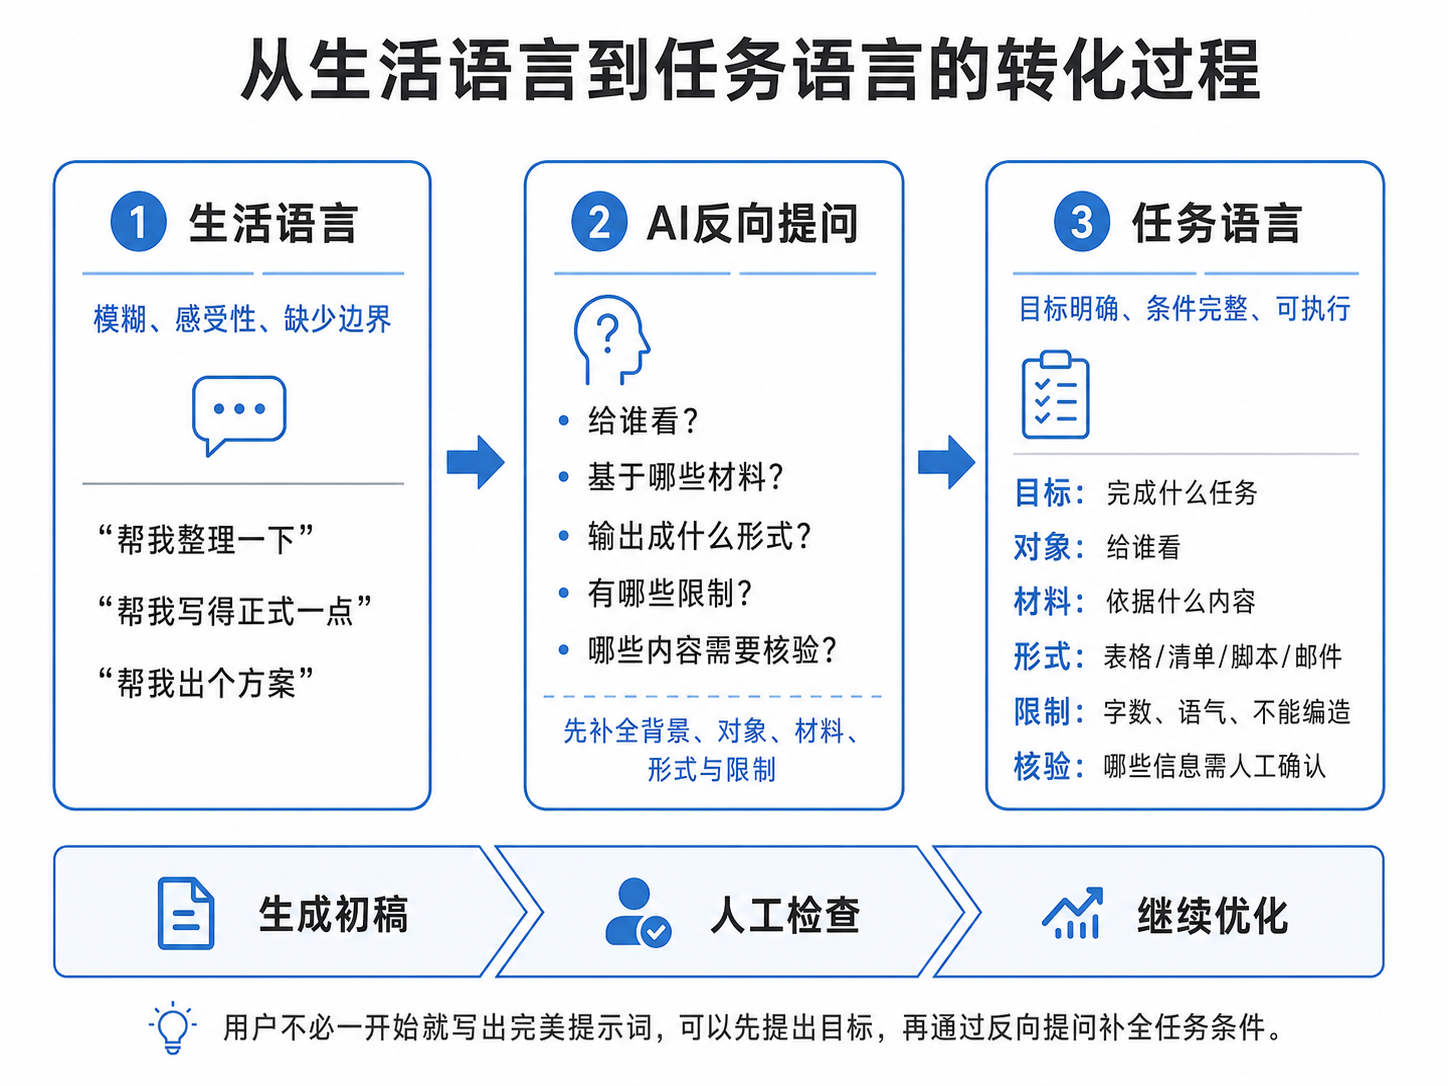
\includegraphics[width=0.88\textwidth]{images_8/ChatGPT Image 2026年5月26日 16_25_33.png}
    \caption{从生活语言到任务语言的转化过程}
    \label{fig:life-to-task-process}
\end{figure}
\FloatBarrier



一些新的 AI 工具已经开始提供提示词生成和提示词优化能力，可以根据任务目标自动补充背景、格式、变量和评价标准。这说明，提示词的使用方式正在从“手写复杂模板”转向“提出目标后由 AI 辅助完善”。

不过，AI 能优化提示词，并不代表用户可以跳过需求拆解。工具只能帮助把指令写得更完整，却不能替人判断真正要解决什么问题、应该提供哪些材料、输出给谁看、哪些内容不能编造、哪些结果需要人工核验。因此，实际使用时，重点不再是记住某个“万能提示词公式”，而是先把目标、材料、格式和限制说清楚，再让 AI 帮助完善指令。

在实际使用中，复杂任务也不宜一次性全部交给 AI 完成。更稳妥的方法，是把大任务拆成几个连续的小步骤。比如制作 AI 短剧，可以先确定主题和故事梗概，再生成角色设定、分镜脚本、画面提示词、配音文案和发布说明；准备会议汇报，可以先整理资料，再提炼观点，接着生成发言提纲，最后改成适合现场表达的口语稿；办理生活事务，可以先梳理材料清单，再生成咨询话术，最后整理注意事项。分步完成的好处是，每一步都可以人工检查和调整，避免 AI 在前一步理解错误的情况下继续生成后续内容。

当一个任务只做一次时，写清楚提示词就可以了；但如果同一类任务会反复出现，就可以把它整理成 Skill。Skill 可以理解为一套可复用的任务说明书，它告诉 AI：什么时候使用这个能力、需要提供什么材料、应该按什么步骤处理、最终输出什么格式，以及哪些内容必须提醒人工确认。

如果后续使用 opencode 这类 Agent 工具，Skill 还可以进一步整理成独立文件或项目规则，让智能体在合适的任务中读取并执行。这样，AI 的使用就不再只是每次临时写一段提示词，而是把常用任务沉淀成可以长期调用的工作流程。

下面以“家乡特产一周内容策划 Skill”为例，完成一次 Skill 构建。

\minorheading{步骤一：选定具体任务}

我要为一个家乡特产设计一周的宣传内容。

可以先打开任意一个 AI 软件官网或者 App，输入下面这句话：

\begin{tcolorbox}[promptbox]
我想为一个家乡特产做一周宣传，但我还没有想清楚具体内容。请你先不要直接写文案，而是先问我 6 个必须确认的问题，帮助我把任务说清楚。
\end{tcolorbox}

这一步的目的不是马上生成结果，而是先让 AI 帮你补全任务条件。围绕“一周宣传内容”这个任务，AI 通常会继续确认几个关键信息：产品是什么、有什么特点、目标人群是谁、准备在哪个平台发布、手里是否已有图片或视频素材、哪些内容不能夸大、哪些信息需要人工确认。把这些问题回答清楚以后，后面的内容计划才会更贴近真实需求。

\begin{figure}[H]
    \centering
    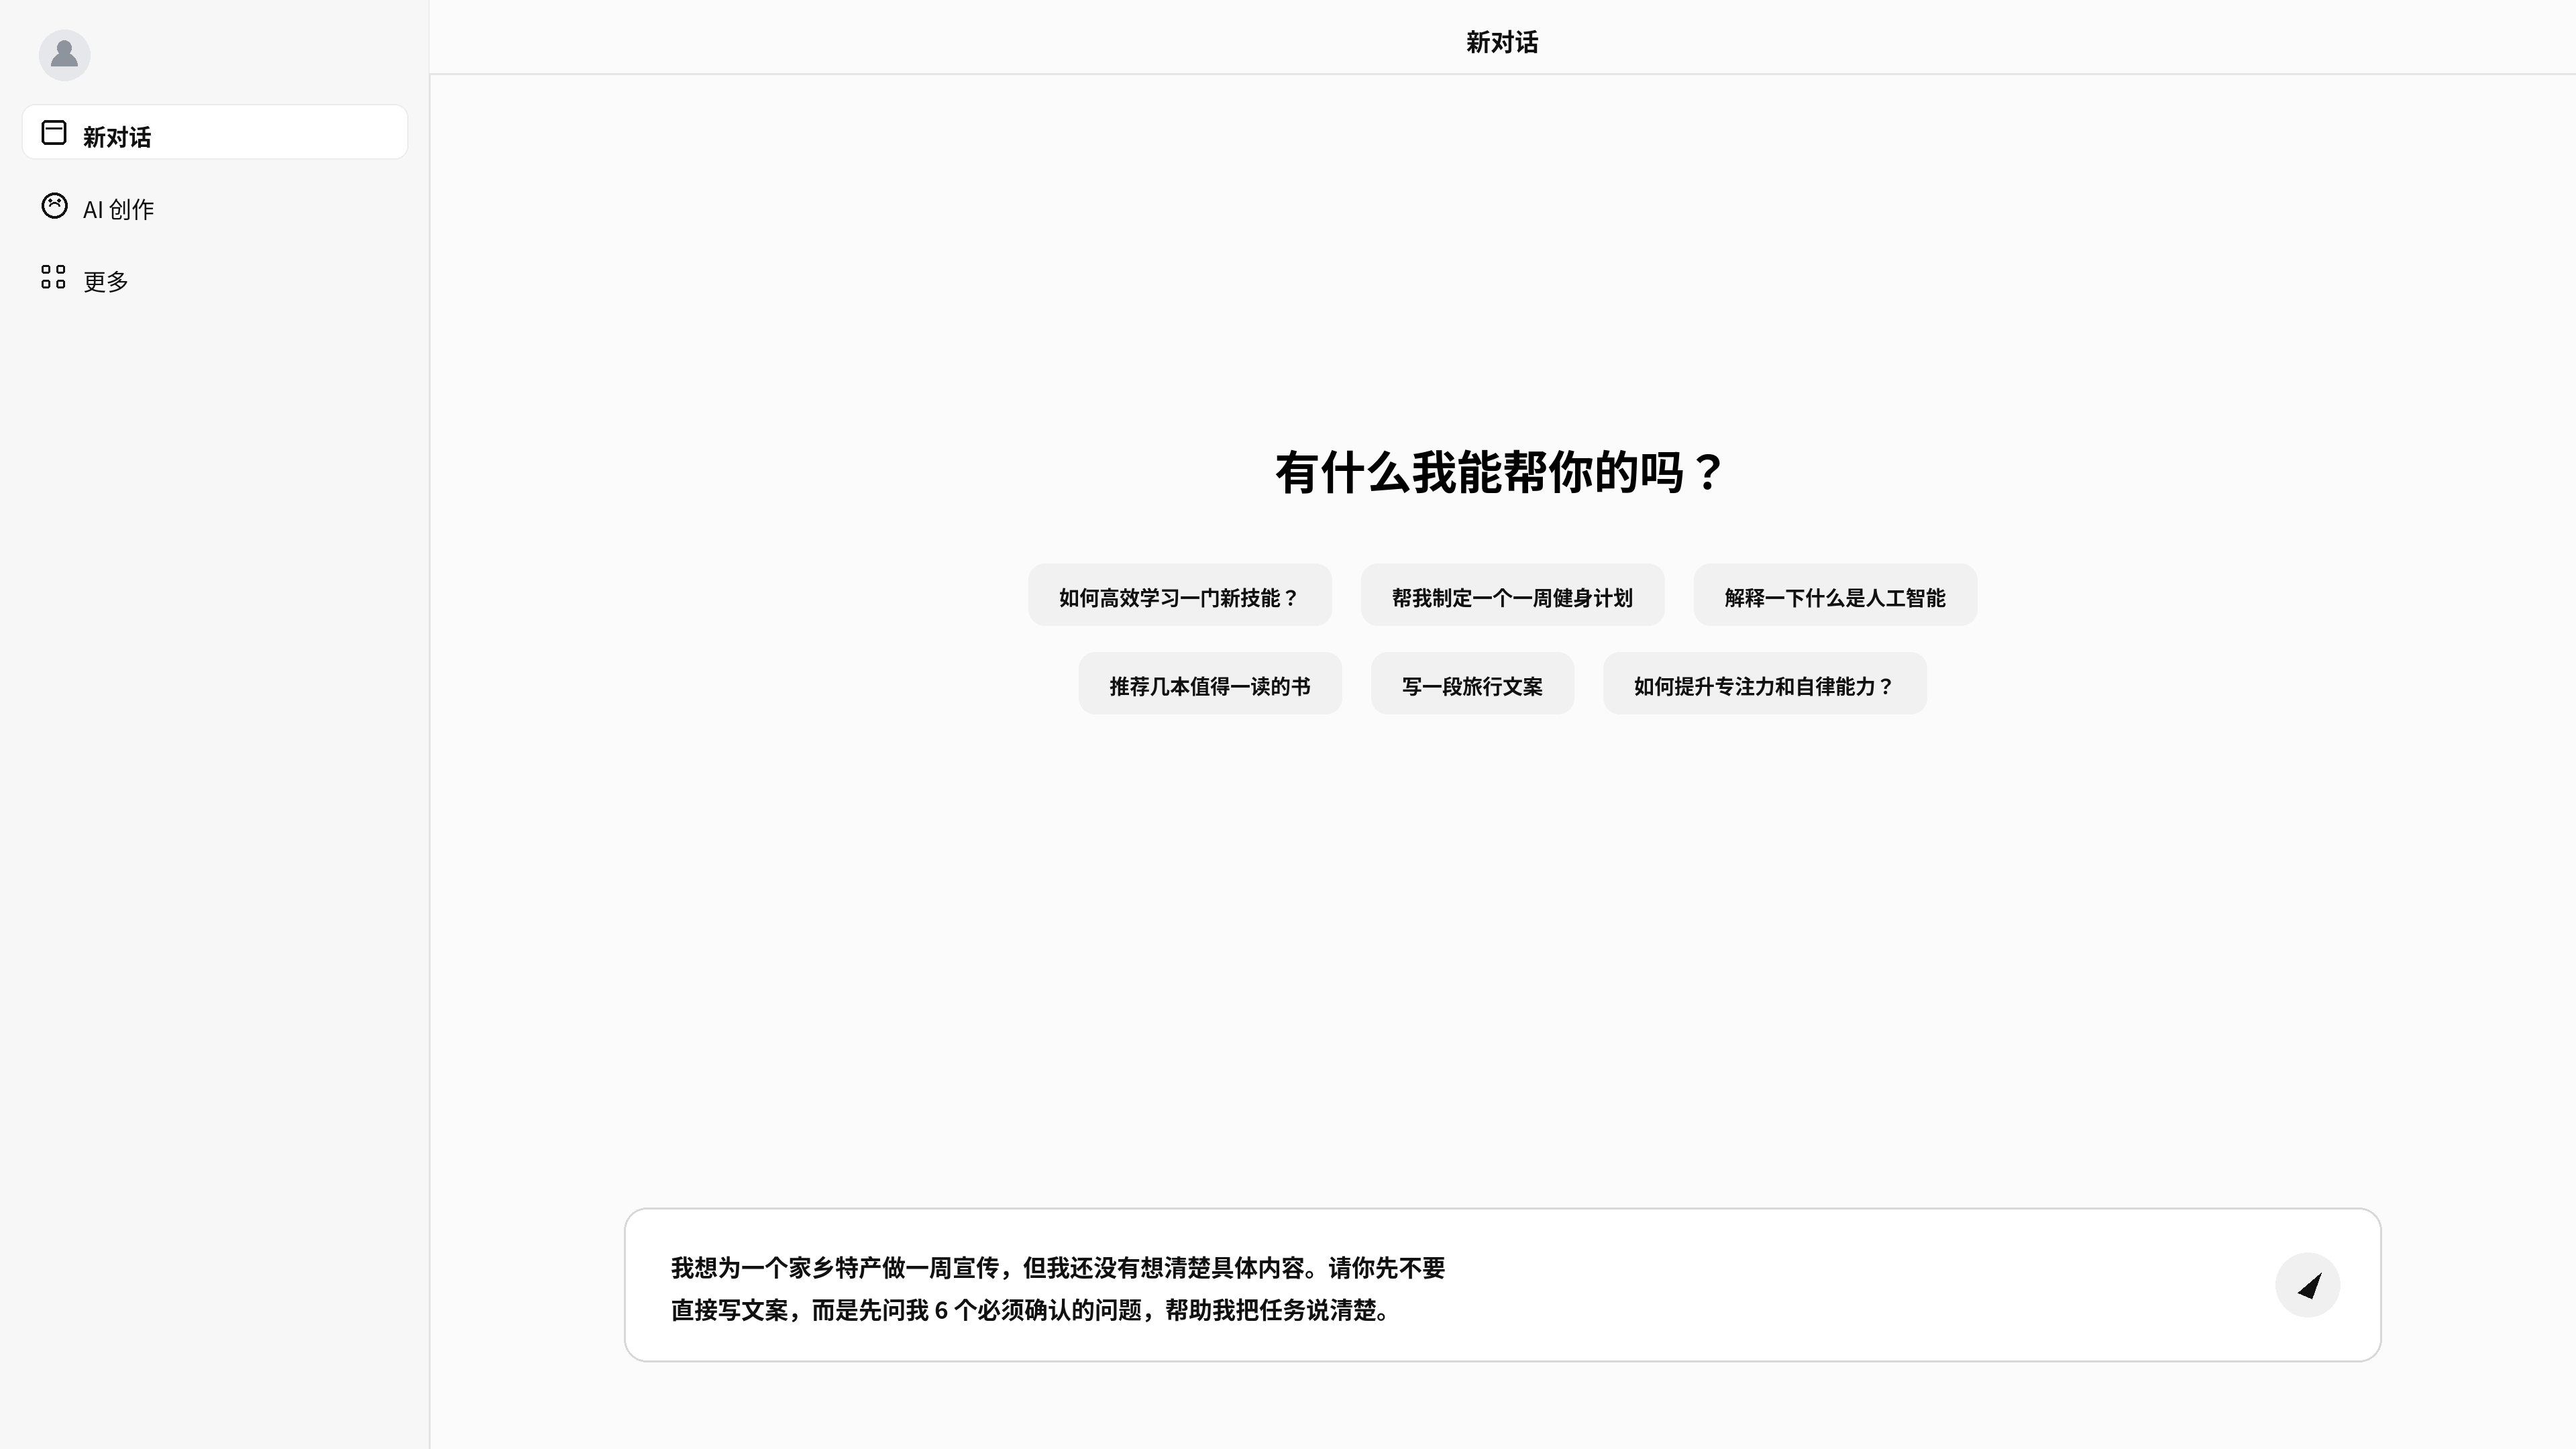
\includegraphics[width=0.88\textwidth]{images_8/步骤1_AI输入界面_4K超高清.png}
    \caption{提出任务目标，让 AI 先反向提问}
    \label{fig:skill-step-question}
\end{figure}
\FloatBarrier

\minorheading{步骤二：补充任务材料}

AI 提出问题后，就可以根据自己的真实情况逐项补充信息。比如，想为家乡特产做一周宣传时，可以这样回答：

\begin{tcolorbox}[promptbox]
产品名称：家乡手工煎饼。

产品特点：薄、脆、有麦香，可以卷菜、卷肉，也可以当零食。

目标人群：年轻上班族、外地游客、想买家乡特产的人。

发布平台：小红书、朋友圈、抖音。

已有素材：有煎饼图片、包装图片、制作过程短视频。

限制条件：不能夸大养生功效，不能编造销量，价格、库存和物流需要人工确认。
\end{tcolorbox}

这样补充以后，AI 获得的就不再是一句模糊的“帮我宣传一下”，而是一组比较完整的任务条件。它知道要宣传什么产品，产品有什么特点，内容写给谁看，准备发到哪些平台，手里有哪些素材，哪些内容不能乱写，哪些信息必须由人确认。

\begin{figure}[H]
    \centering
    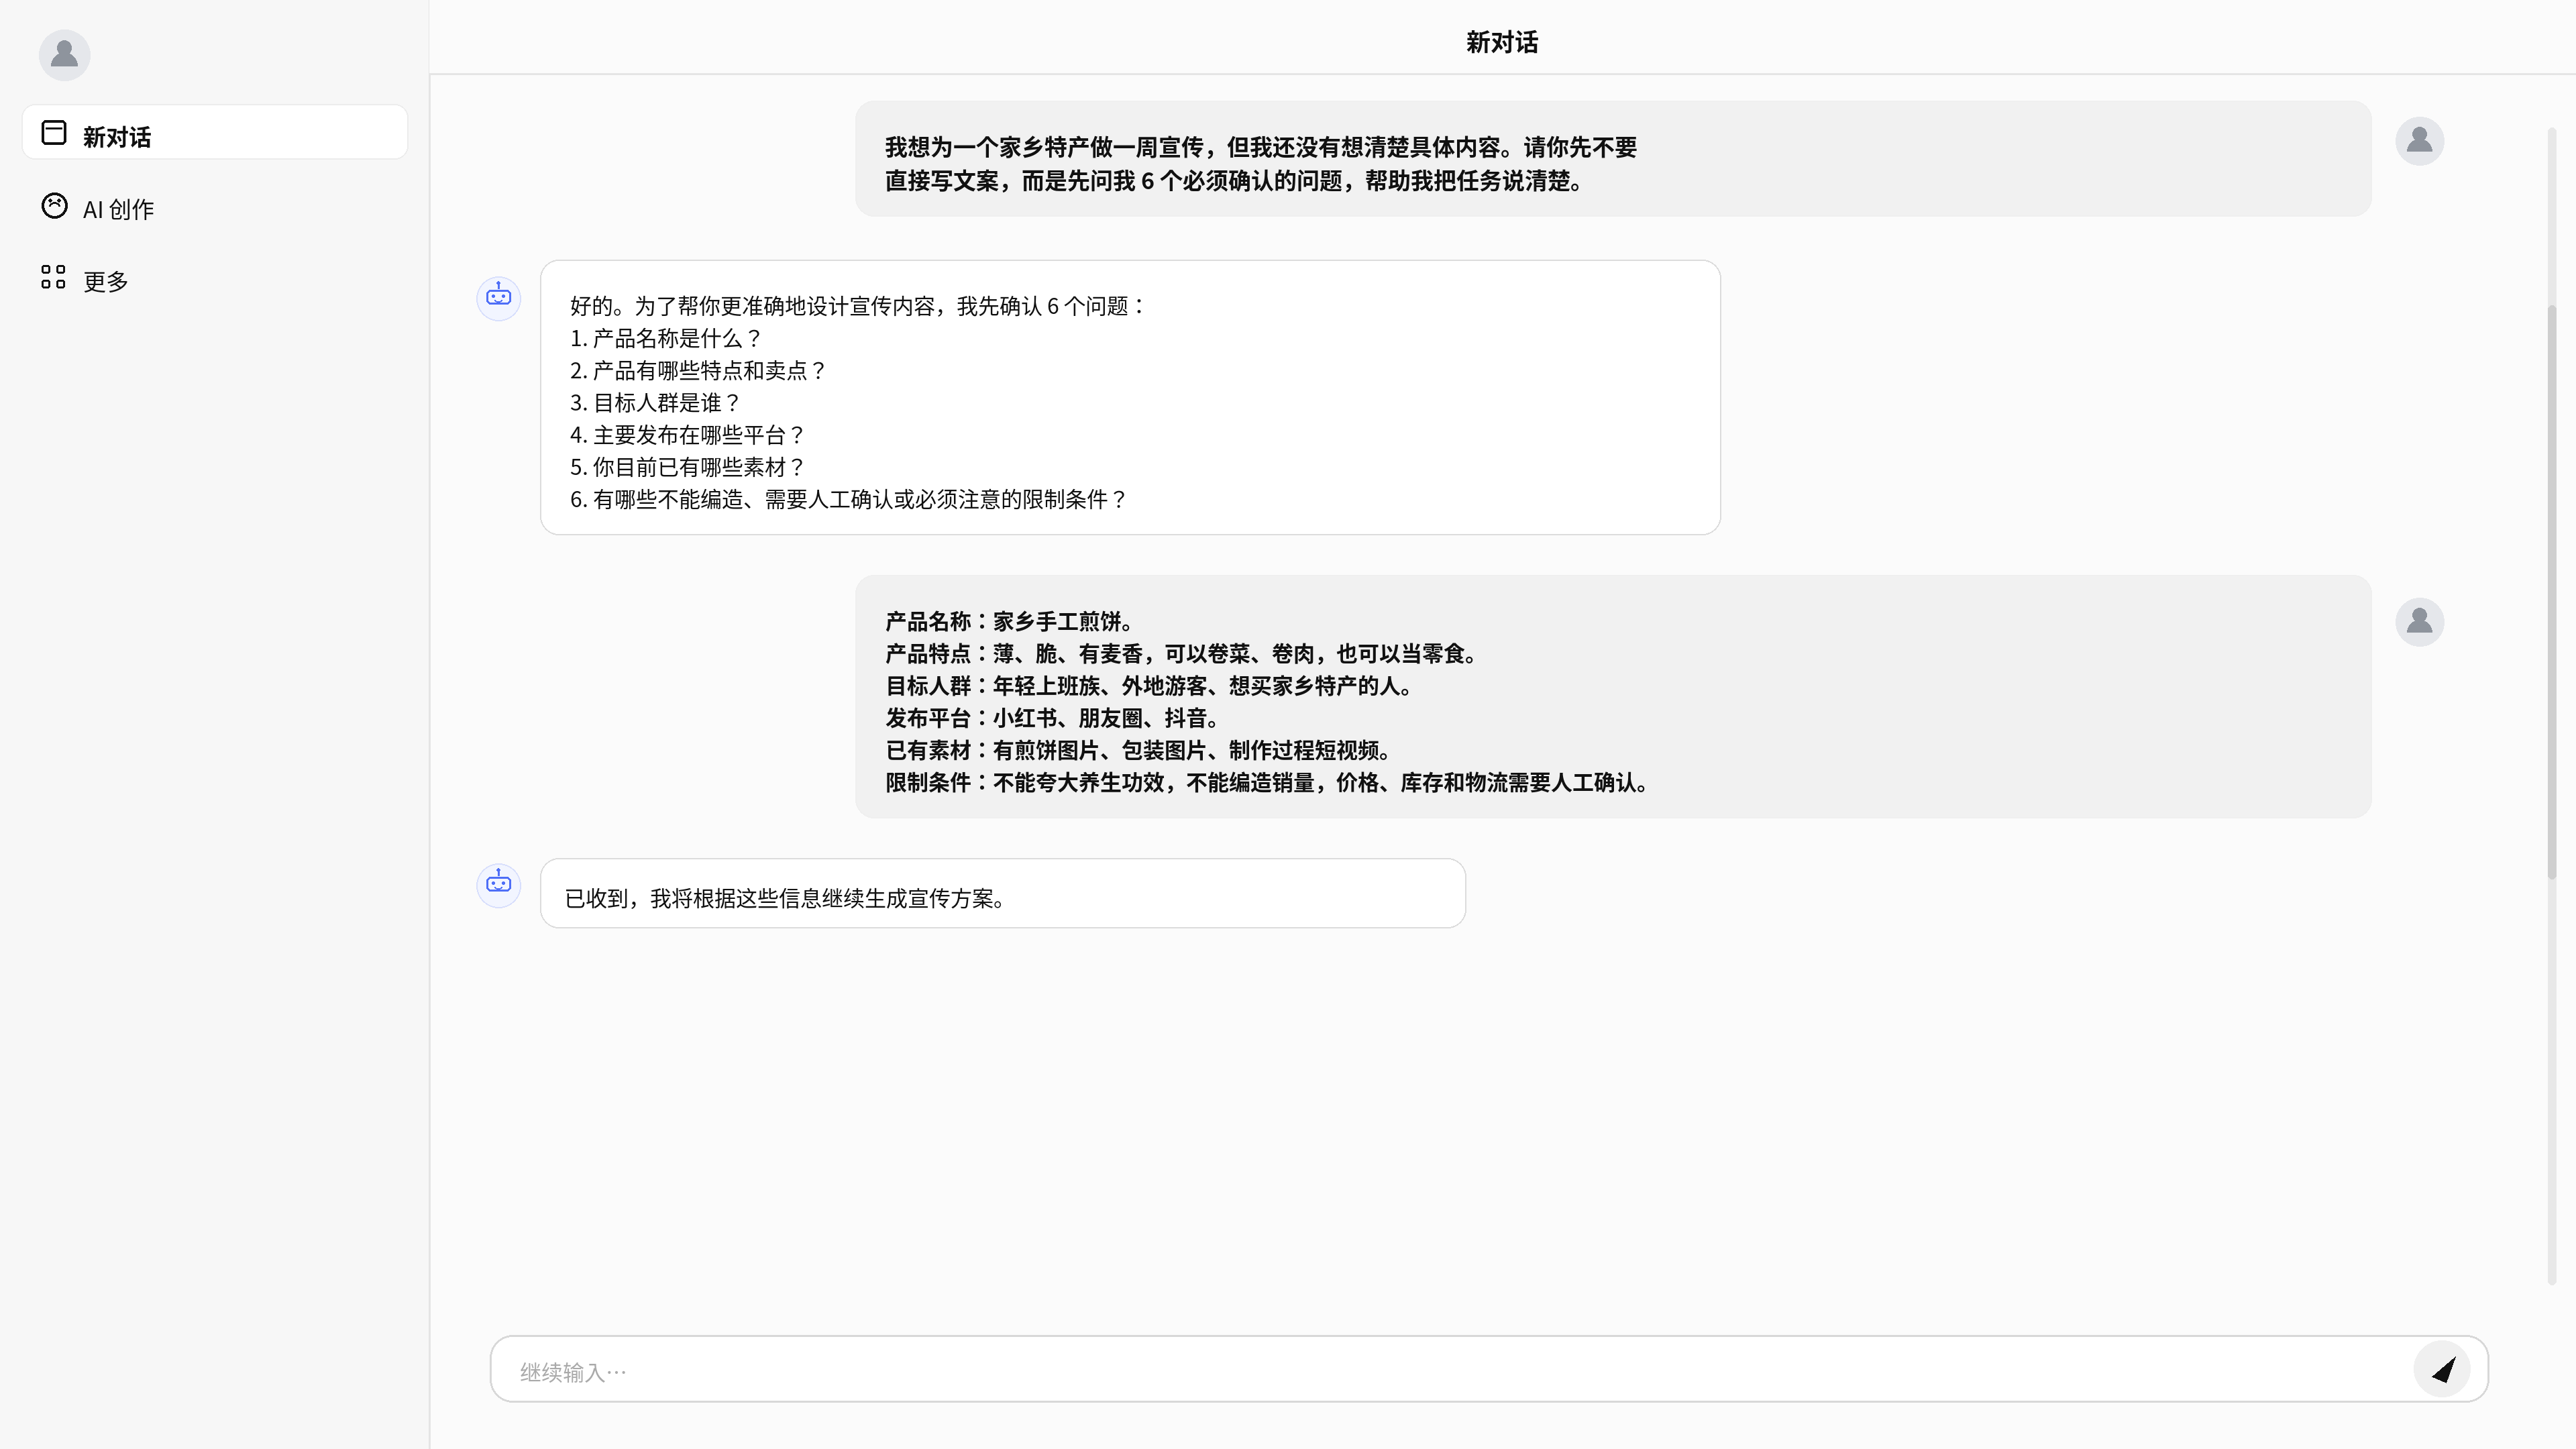
\includegraphics[width=0.88\textwidth]{images_8/步骤2_AI聊天记录界面_4K超高清.png}
    \caption{根据 AI 提问补充任务材料}
    \label{fig:skill-step-material}
\end{figure}
\FloatBarrier

\minorheading{步骤三：生成内容计划}

材料补充完以后，再让 AI 生成第一版结果。可以输入：

\begin{tcolorbox}[promptbox]
请根据我刚才提供的信息，为“家乡手工煎饼”设计一周内容计划。

要求：每天一个不同主题，适合小红书、朋友圈和抖音使用。

请用表格输出，表头包括：日期、内容主题、标题方向、核心文案、短视频脚本方向、素材建议、需要人工核验的信息。

注意：不要编造价格、销量、功效、荣誉和用户评价。
\end{tcolorbox}

这时，AI 生成的结果可能已经比较完整。接下来不能直接照搬，而是检查这份内容计划是否好用。

可以重点看四个问题：

第一，每天的内容是不是重复。

第二，标题是不是适合目标平台。

第三，短视频脚本方向能不能真的拍出来。

第四，有没有把价格、库存、功效、销量等内容标成“需要人工核验”。

如果发现结果太空，可以继续追问：

\begin{tcolorbox}[promptbox]
这些标题有点普通，请改得更适合小红书，但不要夸张，不要像广告。

第 3 天的短视频方向不容易拍，请改成普通手机也能完成的拍法。
\end{tcolorbox}

\begin{figure}[H]
    \centering
    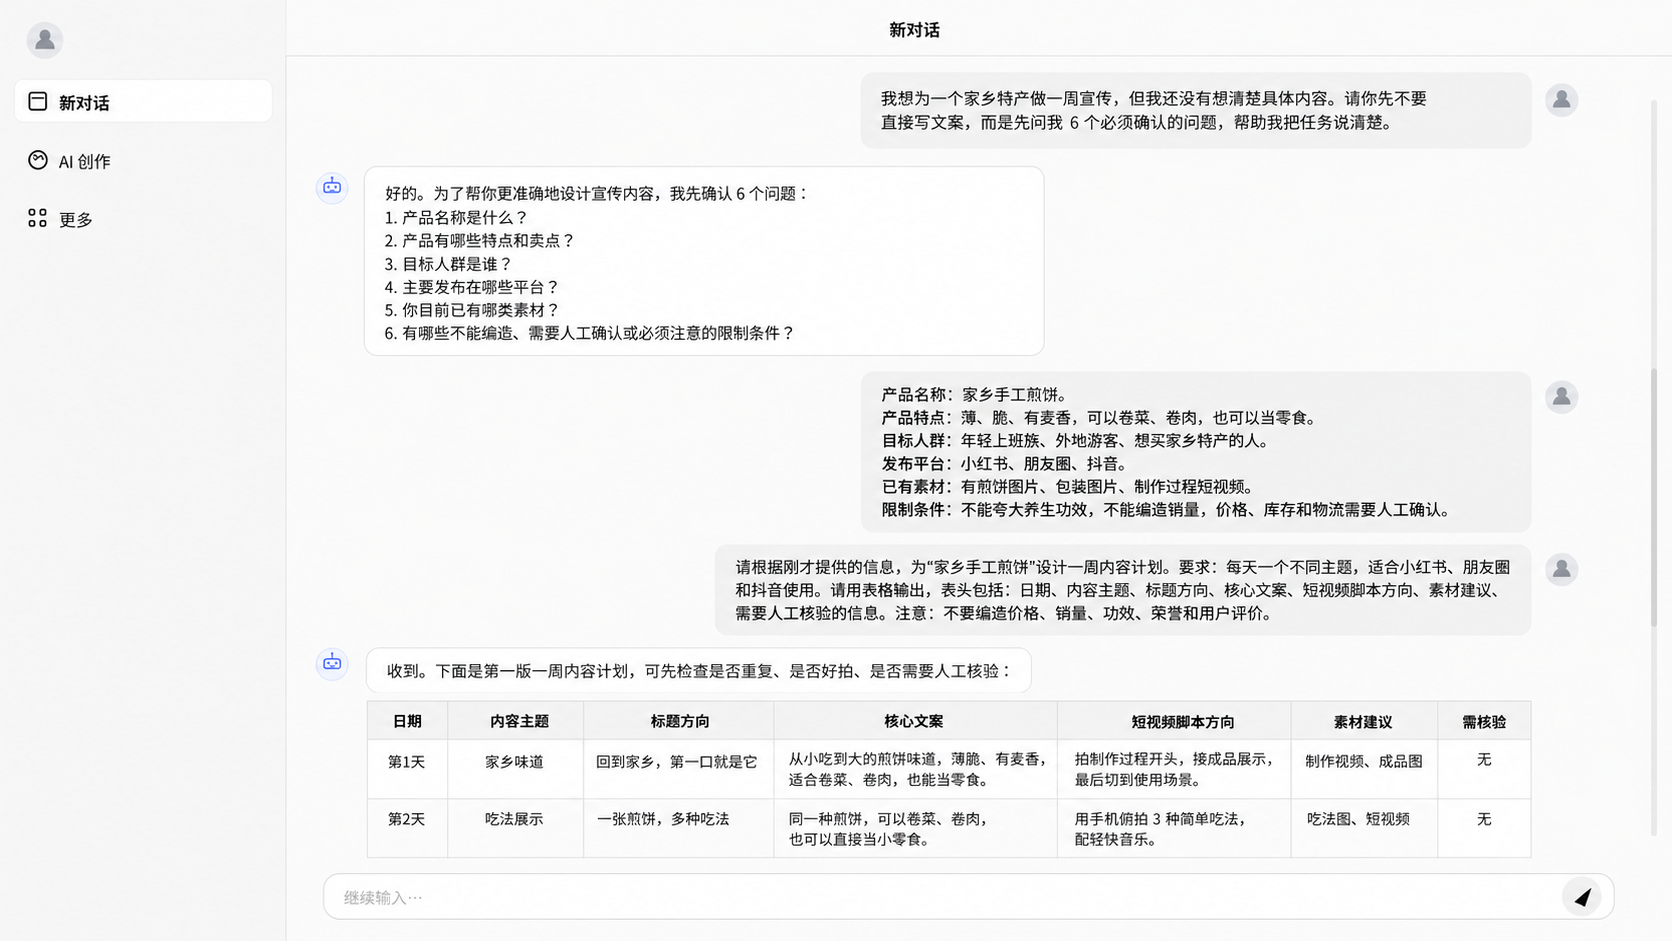
\includegraphics[width=0.88\linewidth]{ChatGPT Image 2026年5月27日 02_12_26.png}
    \caption{生成计划内容}
    \label{fig:placeholder}
\end{figure}

\minorheading{步骤四：沉淀为 Skill}

当这套流程比较好用，就可以把它保存成 Skill。如果不熟悉计算机操作，也不需要一开始就写代码或创建复杂文件夹。最简单的方法是：打开 WPS、备忘录或飞书文档，新建一个文档，标题写成：

\begin{tcolorbox}[promptbox]
家乡特产一周内容策划 Skill
\end{tcolorbox}

然后把下面这份内容复制进去。

\begin{tcolorbox}[skillbox,title=家乡特产一周内容策划 Skill]
\textbf{Skill 名称：} 家乡特产一周内容策划助手

\textbf{适用场景：}

当需要为家乡特产、地方美食、校园文创、非遗产品或轻量经营项目设计一周宣传内容时，使用本 Skill。

\textbf{需要提供的信息：}

产品或主题名称；产品特点；目标人群；发布平台；已有图片、视频或文字资料；推广周期；不能夸大的内容；需要人工确认的信息。

\textbf{执行步骤：}

第一步，先提炼产品或主题的核心卖点，包括产地、口味、使用场景、故事和适合人群。

第二步，判断目标受众关心什么，例如价格、口味、方便程度、送礼价值、地方特色。

第三步，设计一周内容计划，每天一个不同角度，避免重复宣传。

第四步，为每天内容生成标题方向、核心文案、短视频脚本方向和素材建议。

第五步，标出所有需要人工核验的信息。

\textbf{输出格式：}

请用表格输出，表头为：日期、内容主题、标题方向、核心文案、短视频脚本方向、素材建议、需要人工核验的信息。

\textbf{注意事项：}

不要编造价格、库存、销量、荣誉、功效、用户评价和物流承诺。涉及价格、库存、发货时间、功效描述、素材版权和宣传效果的内容，都要标注“需要人工确认”。不要直接替用户发布内容，只提供可修改的策划方案。
\end{tcolorbox}

这一步完成后，就已经拥有了一个最基础的 Skill。它本质上是一份“可反复使用的任务说明书”。以后只要换一个产品，比如“家乡苹果”“地方糕点”“校园文创帆布包”“非遗香包”，都可以继续使用这份 Skill。

需求拆解和指令构建，是后续所有 AI 应用场景的基础。无论是出行规划、学习辅导、生活办事、会议协作，还是职业经营、内容创作和跨文化表达，本质上都需要先把模糊需求变成清晰任务，再让 AI 根据任务要求生成可检查、可修改、可复用的结果。掌握这一方法之后，AI 的使用就不再停留在“想到什么问什么”的临时提问，而会逐渐变成一种有步骤、有标准、能沉淀的智能协作方式。

\subsection{Skill 迭代与能力沉淀}

完成一个 Skill 之后，更重要的事情是让它在以后的任务中持续发挥作用。前面构建的“家乡特产一周内容策划 Skill”，已经把一次临时提问整理成了可复用的任务说明。但真正成熟的 Skill，不只是保存在文档里的一段提示词，而是能够被反复调用、不断修改，并逐渐形成个人 AI 能力库的一部分。

保存 Skill 时，可以先从最简单的方式开始。可以在 WPS、飞书文档、备忘录或网盘中新建一个文件夹，命名为“我的 AI Skill 库”。每一个 Skill 单独保存成一个文档，标题尽量清楚，例如“内容策划 Skill”“短视频脚本 Skill”“客户回复 Skill”“会议纪要 Skill”“发布审查 Skill”。以后遇到类似任务时，不需要重新组织完整提示词，只需要打开对应文档，替换新的主题、材料和限制条件即可。

一个值得长期保存的 Skill，通常有三个特点：第一，这类任务会反复出现；第二，它能明显节省整理和表达的时间；第三，它有相对固定的输出格式和检查标准。比如，随手写一句节日祝福，通常不需要专门保存成 Skill；但整理会议纪要、生成一周内容计划、撰写客户回复、检查发布风险，就很适合沉淀下来。因为这些任务不仅经常出现，而且每次都需要按照一定步骤完成，输出结果也需要保持稳定。

Skill 保存以后，还要在使用中继续修改。比如，“内容策划 Skill”第一次使用时，可能已经能生成一周选题，但标题有些夸张，脚本不方便拍摄，或者风险提示不够明显。这时就可以回到 Skill 文档中补充规则，例如：“标题要自然可信，不使用夸张营销话术”；“短视频脚本应适合普通手机拍摄”；“涉及价格、库存、功效、销量、用户评价和版权素材时，必须标注需要人工确认”。这样，Skill 就会在一次次使用中变得更稳定。

现在一些 AI 平台也开始把提示词生成、提示词优化和结果评估做成工具。比如 OpenAI 的 Prompt Optimizer 可以根据任务目标改进提示词；Anthropic 也在相关文档中强调，智能体应用正在从单纯的 prompt engineering 走向更重视上下文组织、工具说明和持续迭代的 context engineering。这样的趋势说明，AI 使用正在从“写一次提示词”发展为“持续优化任务流程”。实际使用时，不一定要掌握复杂技术，但要形成一个意识：好用的提示词和 Skill 都不是一次写成的，而是在实际任务中不断测试、调整和积累出来的。

当 Skill 越来越多时，还需要学会分类。可以把个人 Skill 库分成几类：“信息整理类”用于整理通知、会议记录、资料和文件；“内容创作类”用于生成选题、脚本、文案和标题；“沟通表达类”用于写邮件、客户回复、求职介绍和会议发言；“检查审查类”用于核对事实、隐私、版权和风险；“复盘总结类”用于记录反馈、总结问题和改进下一步行动。分类的目的不是为了形式整齐，而是为了在真正需要时能够快速找到对应工具。

\begin{figure}[H]
    \centering
    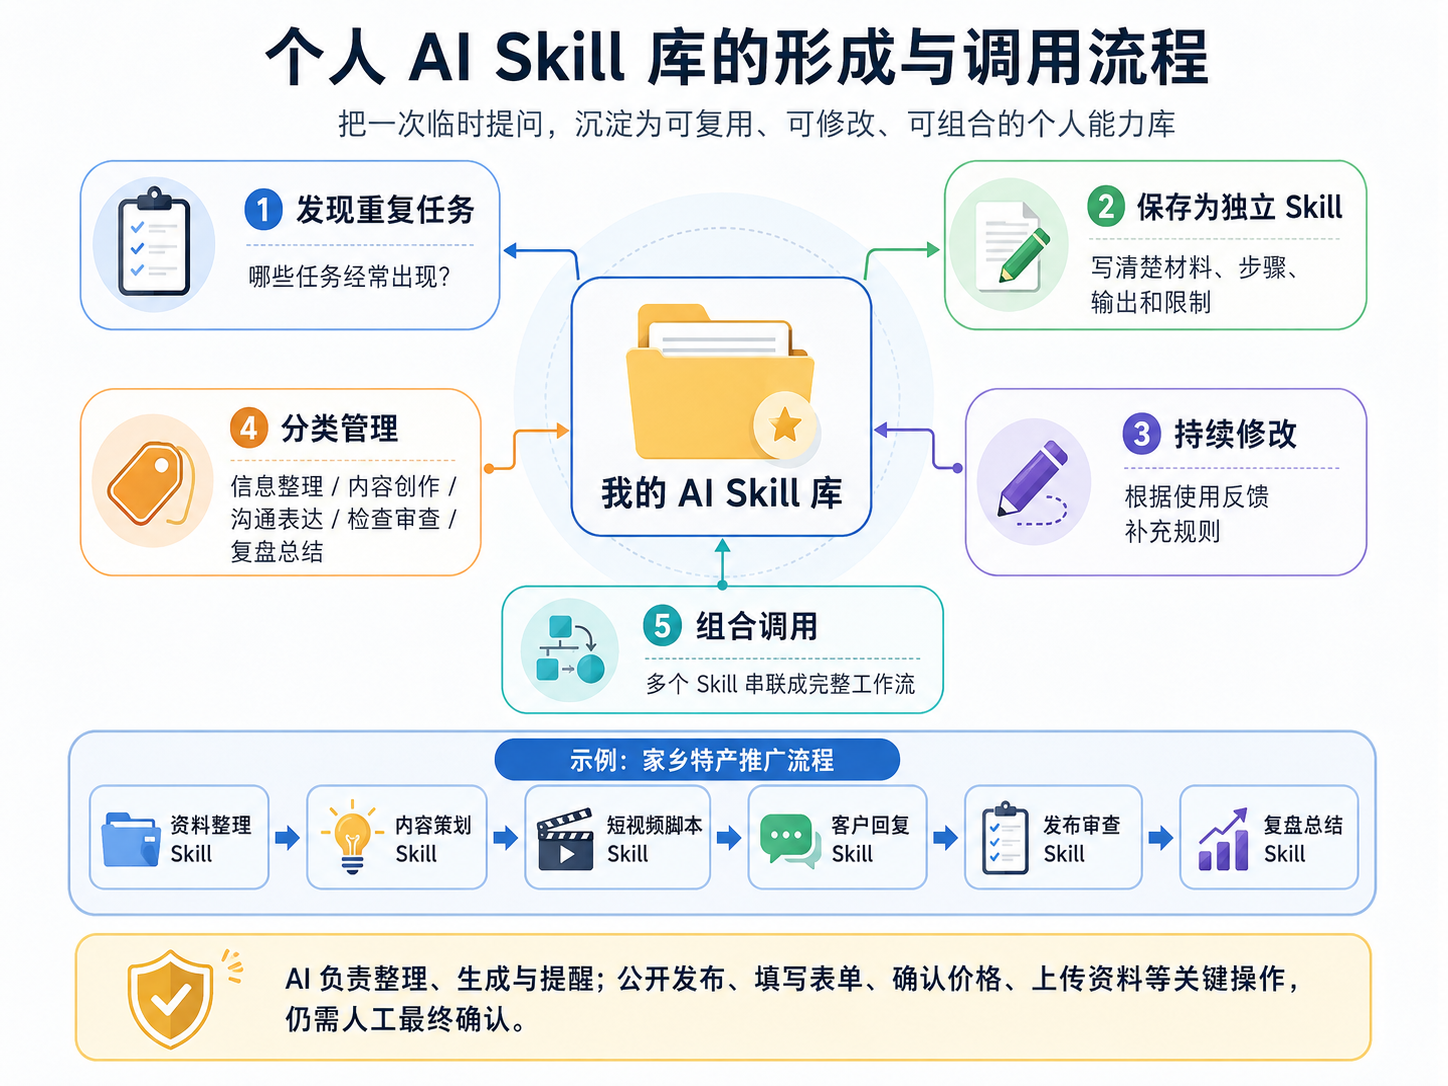
\includegraphics[width=0.88\textwidth]{images_8/8.2.1.png}
    \caption{个人 AI Skill 库的组织与调用流程}
    \label{fig:skill-library-flow}
\end{figure}
\FloatBarrier

单个 Skill 只能完成一个环节，多个 Skill 组合起来，才能形成完整流程。以前面的“家乡特产一周内容策划 Skill”为例，它主要解决“这一周发什么内容”的问题。如果要完成一次完整推广，还需要先用“资料整理 Skill”提炼产品卖点，再用“内容策划 Skill”生成一周选题，用“短视频脚本 Skill”扩写分镜和口播，用“客户回复 Skill”准备常见问答，用“发布审查 Skill”检查事实、隐私、版权和夸大宣传，最后用“复盘总结 Skill”记录发布效果和改进方向。这样，AI 的使用就从一个个孤立任务，逐渐变成一套可以持续运行的个人工作流。

需要注意的是，Skill 的作用是提高效率和稳定性，而不是替人承担责任。整理资料、生成初稿、制作清单、提出建议，通常可以交给 AI 辅助；但涉及公开发布、填写表单、确认价格、承诺服务、上传资料、发送信息等操作时，必须由人进行最终确认。只有把 Skill 管好、改好、组合好，并始终保留人的判断，AI 才能真正成为长期可靠的学习、工作和生活助手。

\section{出行服务与跨语言沟通}

\subsection{行前准备与行程规划}

出行准备看似是一件小事，但很多麻烦都发生在出门之前。有人去医院复查，到了窗口才发现忘带检查报告；有人去政务大厅办业务，排了半小时队才知道还缺一张复印件；有人去考试，路线查得很清楚，却没有考虑早高峰、安检和找考场时间；也有人去陌生城市参加活动，酒店、会场、交通、天气都分开查了一遍，最后还是手忙脚乱。由此可见，出行不是简单的“从哪里到哪里”，而是一个包含路线、时间、材料、流程和突发情况的综合任务。

现在的 AI 出行辅助，已经不再只是导航工具。过去使用地图，主要是为了知道“从哪里到哪里怎么走”；而现在，AI 可以围绕一次出行做更完整的安排。比如去医院复查，可以让 AI 提醒你提前查看挂号时间、准备证件、估算路上时间；去参加会议，可以让 AI 帮你确认地点、规划出发时间、整理需要携带的材料；周末出去玩，也可以让 AI 结合天气、距离和同行人员，帮你选择更合适的路线和活动。这样一来，AI 解决的就不只是“怎么走”，而是“这次出门怎样安排更顺利”。

出发前使用 AI，可以按照\textbf{“一个目标、三类信息、两项确认”}来整理。

\textbf{一个目标}，就是先说清楚这次出门到底要完成什么事情。比如“去医院复诊”“去参加考试”“去办证”“去面试”“去参加活动”。不同目标，对应的准备重点是不一样的。去医院，重点可能是病历、检查报告、医保卡和挂号时间；去考试，重点是准考证、身份证、入场时间和考场位置；去面试，重点是简历、作品集、着装和公司地址；去办证，重点是材料、照片、预约记录和办公时间。目标说得越清楚，AI 才越容易帮你查漏补缺。

\textbf{三类信息}，可以理解成出门前要想明白的三件事：怎么去、带什么、到了怎么办。
第一类是路线信息，包括从哪里出发、几点要到、坐地铁还是打车、需不需要换乘、下车后还要走多远。第二类是材料信息，包括证件、文件、照片、票据、预约记录、证明材料等。第三类是现场信息，比如办公楼在哪一栋、入口在哪里、去几楼、找哪个窗口、是否需要排队、有没有安检要求、附近能不能停车。这样整理以后，出门就不只是“导航到某地”，而是一份更完整的行动安排。

\textbf{两项确认}，是为了避免“AI 说得很顺，但实际用不了”。第一项是官方确认。AI 可以帮你整理和提醒，但不能替代官方通知。时间、地点、材料、费用、预约、考试规则、医院安排等信息，最后都要回到地图实时信息、医院平台、学校通知、政务平台或活动通知中核对。第二项是备用方案确认。比如堵车怎么办，地铁临时停运怎么办，材料少带了怎么办，手机没电了怎么办。提前让 AI 帮你想一遍这些情况，真正出门时就不容易手忙脚乱。

下面选取医院复诊、考试和政务办事三个常见场景，说明 AI 如何把出门前容易遗漏的事项整理成清单。

如果是去医院复诊，可以这样输入：

\begin{tcolorbox}[promptbox]
明天上午 9 点我要去医院复查，从家里出发，最好提前 20 分钟到。请帮我整理一份出门前准备清单，包括建议出发时间、交通路线、可能需要带的材料、要问医生的问题、路上可能出现的风险和备用方案。不能确定的信息请标注“需要我自己确认”。
\end{tcolorbox}

这类清单可以包括四个部分：一是出发时间和路线安排，例如是否需要预留早高峰、排队和找科室的时间；二是需要携带的材料，例如身份证、医保卡、挂号记录、检查报告、病历本和正在服用的药物清单；三是复诊时想咨询的问题，例如症状是否加重、药物是否需要调整、是否需要复查项目；四是备用方案，例如交通拥堵时是否改乘地铁、找不到科室时如何询问导诊台、预约信息不一致时如何处理。

如果是参加考试，可以换成下面这个提示：

\begin{tcolorbox}[promptbox]
我明天上午要参加考试，9 点开始，考点在某某学校。我从家出发，请帮我整理出行准备清单，包括建议出发时间、交通方案、需要携带的证件和文具、考前注意事项、迟到风险和备用方案。请提醒我哪些信息必须再去准考证或官方通知中核对。
\end{tcolorbox}

这类提示的重点，是让 AI 把“出门”拆成几个可检查的环节。考试场景中，路线只是其中一项，更重要的是准考证、身份证、文具、入场时间、考场位置、安检要求、禁止携带物品和迟到后果。AI 可以帮你列出清单，但最终仍要以准考证和考试官方通知为准。

如果是去政务大厅办事，可以这样输入：

\begin{tcolorbox}[promptbox]
我准备去政务大厅办理业务，但不确定要带什么材料。请帮我整理出门前需要确认的内容，包括办理地点、办公时间、可能需要的证件、复印件、照片、线上预约、咨询电话和现场排队风险。不能确定的信息请标注“需要官方确认”。
\end{tcolorbox}

这时，AI 的作用是提前形成一份“办事检查表”。它可以提醒我们确认：是否需要原件和复印件，是否要提前预约，是否必须本人到场，是否需要照片，能不能线上办理，是否有午休时间，到现场后是否需要取号排队。

这些问题看似琐碎，却往往决定一次出门能不能顺利完成。很多办事失败，并不是因为找不到地方，而是因为材料、时间或流程没有提前确认。

前面已经学习过，反复出现的任务可以整理成 Skill。接下来，我们就以更常见的\textbf{“出门旅行”}为例，看看如何把目的地、交通、住宿、预算、天气、预约、行李和备用方案等内容，整理成一个可以反复使用的\textbf{“出门旅行计划 Skill”}。这样以后再做旅行计划时，就不必每次都从零开始问 AI，而是可以让 AI 按照固定流程生成更稳定、更实用的结果。

\minorheading{旅行 Skill：固化行程流程}

制作这个 Skill 时，可以先打开 WPS、飞书文档、备忘录或手机便签，新建一个文档，标题写成：

\begin{tcolorbox}[promptbox]
出门旅行计划 Skill
\end{tcolorbox}

然后把下面这段内容保存进去：

\begin{tcolorbox}[skillbox,title=出门旅行计划 Skill]
你是“出门旅行计划助手”。我会告诉你旅行目的地、出发地、旅行时间、同行人员、预算、兴趣偏好和限制条件。请你帮我整理一份适合普通人执行的旅行计划。

请按照以下步骤完成：

第一步，先概括本次旅行目标，包括去哪里、玩几天、和谁去、主要想体验什么。

第二步，整理出发前需要确认的信息，包括交通方式、住宿位置、天气、门票预约、开放时间、身份证件、行李物品和预算。

第三步，设计每日行程安排。每天的安排要包括上午、下午、晚上三个时间段，并说明每个地点之间的大致衔接方式。行程不要排得太满，要给吃饭、休息、排队和临时调整留出时间。

第四步，整理旅行准备清单，包括证件、衣物、充电设备、常用药品、雨具、防晒用品、现金或支付方式、必要票据等。

第五步，给出备用方案。比如天气不好怎么办、景点没预约上怎么办、同行人走累了怎么办、交通延误怎么办。

第六步，标出所有需要人工确认的信息。凡是涉及车票、酒店、门票、开放时间、价格、天气、交通变化和安全提醒的内容，都必须标注“需要确认”，不能自行编造。

请用表格和清单结合的方式输出，语言要清楚、实用，不要写成广告式旅游攻略。
\end{tcolorbox}

保存好\textbf{“出门旅行计划 Skill”}以后，每次旅行前都可以再次调用它。操作时，先打开一个支持文档上传或长文本输入的 AI 工具，把自己保存的 Skill 文档上传给 AI，或者直接复制到对话框中，作为参考材料提供给 AI。

接着，再补充这一次旅行的真实信息，让 AI 按照 Skill 文档里的步骤生成旅行计划。这个过程的核心是：先让 AI 理解“工作规则”，再让它处理“这一次的具体任务”。这样生成出来的计划，就不会完全依赖 AI 临时发挥，而是会沿着我们提前设计好的流程进行。

例如，上传或提供\textbf{“出门旅行计划 Skill”}文档后，可以继续输入：

\begin{tcolorbox}[promptbox]
我已经提供了“出门旅行计划 Skill”文档。请你先阅读并理解里面的流程，然后按照这个 Skill 的步骤，帮我规划这次旅行。

本次旅行信息如下：

目的地：青岛

出行时间：7 月 10 日到 7 月 13 日

同行人员：两名成年人

预算：中等

偏好：海边、城市散步、本地小吃，不想行程太赶

交通方式：高铁往返

请先检查我提供的信息是否完整，如果还缺少关键信息，请先提问；如果信息已经足够，请按照 Skill 文档生成旅行计划。
\end{tcolorbox}

\begin{figure}[H]
    \centering
    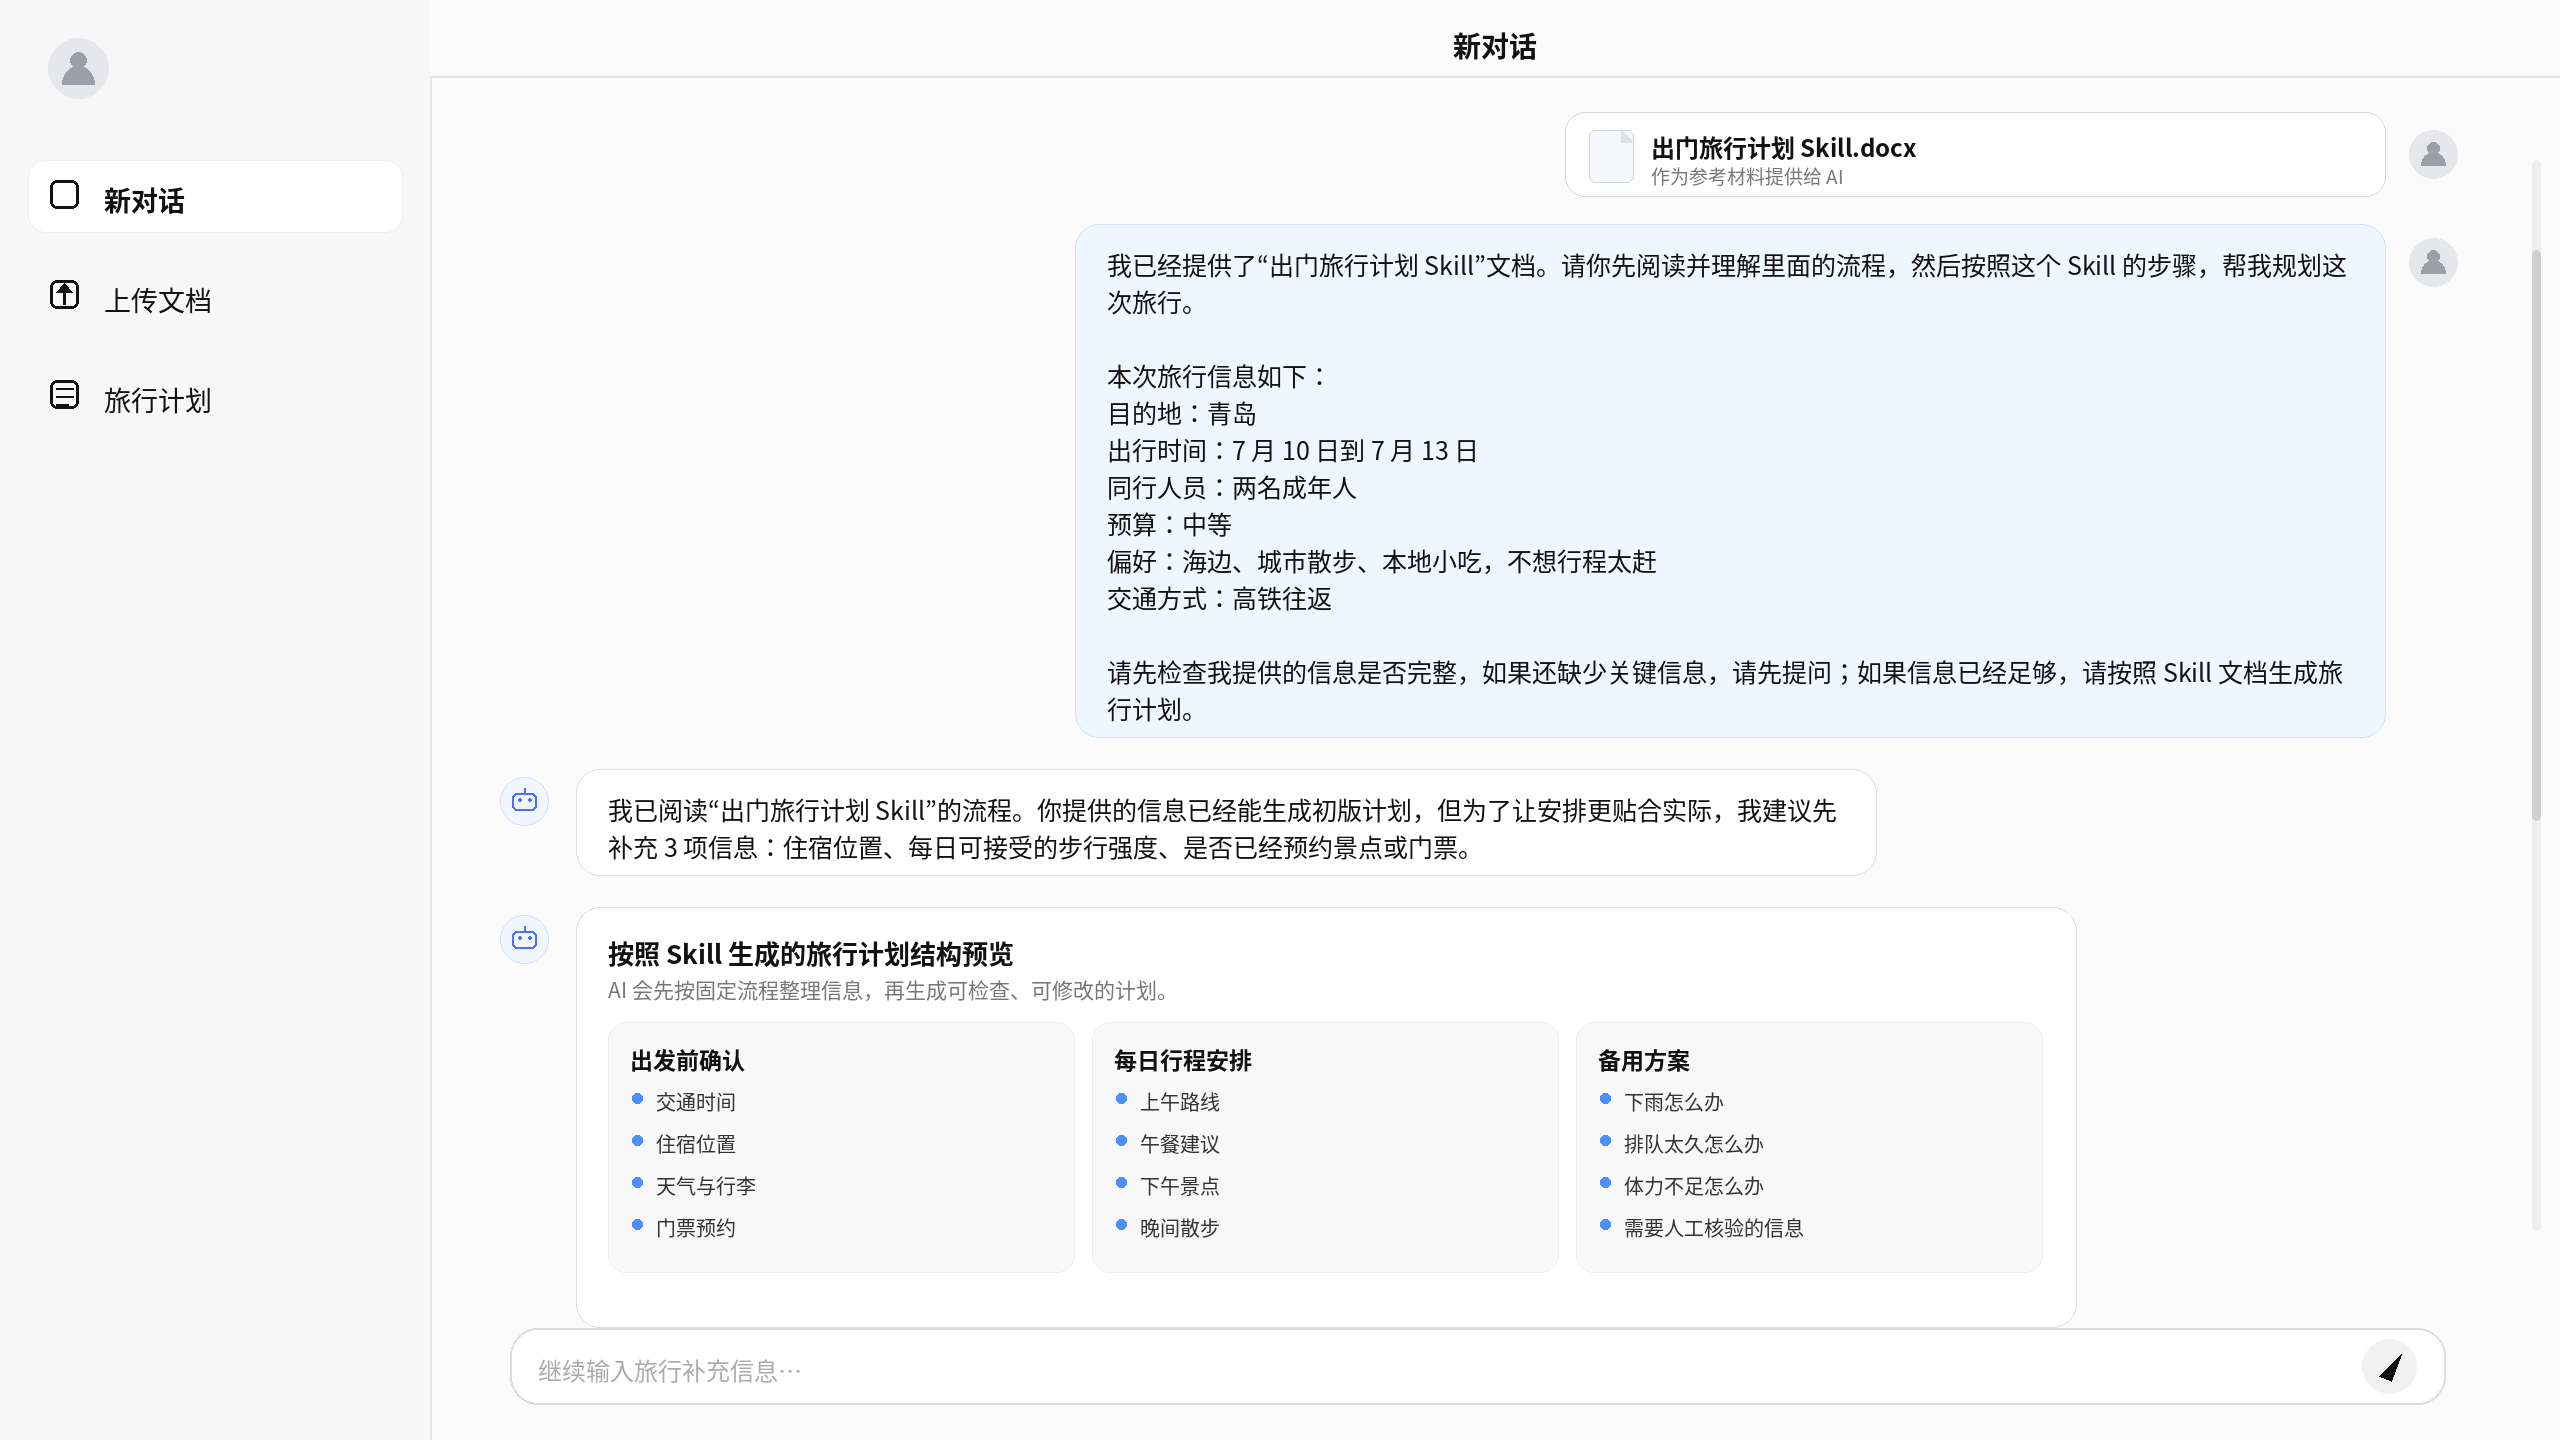
\includegraphics[width=0.88\textwidth]{images_8/出门旅行计划Skill_调用示例_AI界面_2K高清版.png}
    \caption{调用出门旅行计划 Skill 生成行程规划示例}
    \label{fig:travel-skill-call}
\end{figure}
\FloatBarrier




如果是出国旅游，也可以把一些国外平台的 AI 行程规划功能作为辅助工具。例如，Google 在 AI Mode 中加入了 Canvas 旅行规划功能。使用时，只需要描述目的地、旅行时间、预算和偏好，系统就可以生成一份可继续编辑的行程草稿。它不是简单写一段旅游攻略，而是把航班、酒店、地图照片、用户评论和网页资料整合到同一个行程工作区里，帮助你比较住宿、餐厅、活动和路线安排；如果后面想调整计划，也可以继续追问，让系统根据新的需求修改行程。这样，出国旅行时就不必在搜索页面、地图、酒店网站和点评信息之间反复切换，而是可以把它当作一个可持续修改的旅行规划板来使用。

\subsection{在途沟通与即时协同}

出行计划解决的是“出发前怎么安排”，而真正走到路上之后，AI 还可以继续发挥作用。很多时候，旅途中最让人卡住的，并不是目的地没有选好，而是现场突然出现的小问题：看不懂一张菜单，不知道售票机哪个按钮是确认付款，酒店自助入住说明太长，景区公告临时变更，药店标签看不明白，或者餐厅预约需要和店员沟通。尤其是在国外旅行时，这些问题会更加明显，因为语言、规则和操作方式都可能和自己熟悉的环境不同。

这时，AI 的角色就从“行前规划助手”变成了“现场沟通助手”。它不再只是安排路线和行程，而是帮助我们看懂现场信息、生成沟通话术、拆解操作步骤，并提醒哪些内容需要向工作人员确认。例如，手机里的翻译工具已经可以通过摄像头识别菜单、标识牌和说明文字；一些翻译应用也支持实时对话、图片翻译和离线语言包，适合在旅行中处理菜单、街道标识和简单交流问题。

\minorheading{菜单点餐：翻译菜名，判断食材}

在境外餐厅点餐时，菜单往往不是简单的文字翻译问题。许多菜名带有地方特色、烹饪习惯或文化背景，即使被翻译成中文，也未必能让人准确判断它的主要食材、制作方式、口味特点以及是否包含忌口成分。因此，使用 AI 处理菜单时，不宜只停留在“翻译菜名”，而应进一步让 AI 帮助解释菜品内容，并标出需要向服务员确认的信息。

可以这样输入：

\begin{tcolorbox}[promptbox]
我在国外餐厅，请根据我上传的菜单图片，用中文解释每道菜大概是什么。请说明主要食材、烹饪方式、口味可能偏甜/偏辣/偏酸/偏咸，并标出可能含有酒精、海鲜、坚果、牛奶、鸡蛋或生食的菜品。不能确定的地方，请标注“需要向服务员确认”。
\end{tcolorbox}

通过这样的提问，AI 给出的结果就不只是菜单译文，而是一份更接近“点餐辅助说明”的内容。它可以帮助判断某道菜属于主食、汤品、甜点、冷盘还是炸物，也可以提醒某些酱汁、汤底、甜品或腌制食品中可能含有酒精、牛奶、坚果、海鲜等成分。对于有过敏、忌口、宗教饮食或儿童饮食需求的人来说，这类提醒尤其重要。

不过，AI 对食材和过敏原的判断只能作为初步参考，不能代替餐厅确认。菜单图片不清晰、菜名缩写、地方方言、特殊烹饪方式和隐含配料，都可能影响识别和翻译结果。涉及花生、坚果、海鲜、牛奶、鸡蛋、生食、酒精等重要信息时，应当向服务员再次确认。

现场点餐时，还可以让 AI 生成简短、礼貌、便于直接使用的外语表达。例如：

\begin{tcolorbox}[promptbox]
请帮我生成一句英文，用来询问服务员：这道菜是否含有花生？如果含有花生，请推荐一道不含花生的菜。语气礼貌，句子简单，适合现场直接说。
\end{tcolorbox}

AI 可能生成如下表达：

\begin{tcolorbox}[promptbox]
Excuse me, does this dish contain peanuts? If it does, could you recommend a dish without peanuts?
\end{tcolorbox}

点餐类表达不需要复杂，关键是把核心信息说清楚。一般可以按照“想点什么、不能吃什么、需要确认什么”三个部分来组织。也可以提前让 AI 准备几类常用句子：

\begin{tcolorbox}[promptbox]
我不吃生食，请问这道菜是全熟的吗？

我不太能吃辣，请问这道菜可以做成不辣的吗？

我对海鲜过敏，请问这道菜里有没有虾、蟹或鱼露？

我想点一份适合孩子吃的菜，请问哪一道比较清淡？
\end{tcolorbox}

在餐厅场景中，AI 的作用是帮助看懂菜单、理解菜品、准备问句，并降低现场沟通压力；但最终能否食用、是否含有过敏原、是否符合个人饮食要求，仍然需要以餐厅工作人员的确认结果为准。

\minorheading{现场公告：读懂文字，明确行动}

旅行中还有很多信息不是菜单，而是提示牌、交通公告、景区规则、酒店说明、药店标签、商场指示和安全提醒。这类文字往往很短，但影响很大。比如车站屏幕提示某列车换站台，景区入口写着今日部分区域关闭，酒店门口贴着自助入住说明，药品包装上写着服用方式。如果只是逐字翻译，你可能仍然不知道下一步该做什么。

这类场景中，可以让 AI 不只翻译文字，还要解释“这条信息对我有什么影响”。例如，在车站看到公告时，可以输入：

\begin{tcolorbox}[promptbox]
我在车站，请根据我上传的公告图片，帮我判断这条通知和我有什么关系。请用中文说明：它在提醒什么，我是否需要换站台、改路线或重新确认车次，哪些信息必须向工作人员确认。
\end{tcolorbox}

如果是在景区看到提示牌，可以输入：

\begin{tcolorbox}[promptbox]
请根据我上传的景区提示牌，帮我说明这里是否可以进入、是否需要预约、是否有时间限制、是否有安全注意事项。不能确定的地方请标注“需要向工作人员确认”。
\end{tcolorbox}

如果是在酒店自助入住区看到说明，可以输入：

\begin{tcolorbox}[promptbox]
请根据我上传的酒店自助入住说明，帮我整理操作步骤。请告诉我先做什么、后做什么，需要准备哪些信息。涉及护照、信用卡、押金、房间号和验证码的地方，请提醒我自己确认，不要替我判断。
\end{tcolorbox}

这里体现的是 AI 的“现场理解”能力。它不只是把外语变成中文，而是帮助你把外文说明转换成行动步骤：先去哪儿、按什么按钮、准备什么材料、哪些地方要停下来确认。对于旅行者来说，这比单纯翻译更有实用价值。

不过，现场公告和规则具有很强的时效性。车站信息可能几分钟后更新，景区规则可能因为天气和人流临时变化，酒店入住说明也可能因房型、订单和平台不同而不同。因此，AI 可以帮助理解，但不能替代现场工作人员或官方平台的确认。

\minorheading{自助设备：识别界面，谨慎操作}

国外旅行中，自助设备是很常见的难点。自动售票机、自助点餐机、自动贩卖机、地铁充值机、行李寄存柜、投币洗衣机，看起来只是几个按钮，但如果语言不熟，很容易不知道哪个是购买、哪个是取消、哪个是确认付款、哪个是返回上一步。

遇到这类问题时，不要让 AI 直接替自己决定“应该按哪个按钮”。更稳妥的做法，是让 AI 先解释界面，再整理可能的操作步骤。比如面对自动售票机，可以输入：

\begin{tcolorbox}[promptbox]
我面前是一台自助售票机，请根据我上传的屏幕图片，帮我解释每个按钮大概是什么意思，并整理一个安全的操作顺序。不要替我决定购买哪张票。涉及目的地、时间、金额、支付和退款的地方，请标注“需要我自己确认”。
\end{tcolorbox}

AI 能帮助你做到几个层次：先识别界面文字，例如“选择语言”“单程票”“往返票”“确认”“取消”“付款”；再解释按钮功能，例如哪个是继续、哪个是返回、哪个会进入支付；最后整理操作顺序，例如先选择语言，再选择目的地，再选择票种和数量，最后核对金额并付款。

如果是自动贩卖机或自助点餐机，可以这样输入：

\begin{tcolorbox}[promptbox]
请根据我上传的机器界面，帮我说明如何选择商品、如何确认数量、如何付款、如何取消操作。请特别提醒哪些按钮可能是确认付款或取消订单。
\end{tcolorbox}

如果是行李寄存柜，可以这样输入：

\begin{tcolorbox}[promptbox]
我在使用行李寄存柜，请根据屏幕图片帮我解释操作步骤。请提醒我哪些地方涉及付款、取件密码、柜门编号和超时费用，不能确定的地方标注“需要现场确认”。
\end{tcolorbox}

这类场景中，AI 能使用到的程度是“辅助理解界面和步骤”，而不是“替用户完成操作”。最终选择商品、票种、数量、金额、支付方式，都必须由自己确认。尤其是涉及付款、退款、押金、密码、取件码和身份信息时，不要把完整敏感信息上传给 AI，也不要在没有核对清楚的情况下直接点击确认。

\minorheading{预约核对：组织表达，核对凭证}

旅行中经常需要预约餐厅、修改时间、说明迟到、确认订单。很多人不怕吃饭，怕的是打电话、发消息或到店解释不清楚。AI 在这里的价值，是把中文想法整理成清楚、礼貌、适合现场使用的外语表达。

现在一些平台已经开始把 AI 用到预订环节。Google 在 AI Mode 中推出过餐厅预约相关的 agentic 功能，你可以描述人数、时间、地点和菜系偏好，系统会搜索多个预订平台，展示可订选项，并引导到对应页面完成最终预订。Booking.com 也推出了 AI Trip Planner、AI Voice Support、Smart Messenger、Auto-Reply 和 AI Trip Support 等功能，用于旅行规划、住宿沟通和行程支持。

实际使用中，可以先让 AI 生成预约表达。例如：

\begin{tcolorbox}[promptbox]
请帮我写一段英文餐厅预约信息。内容是：我想预约今晚 7 点，两个人，尽量靠窗，其中一位不吃海鲜。如果不能安排靠窗，也可以接受普通座位。语气礼貌、简短。
\end{tcolorbox}

AI 可以帮助生成一段适合发送给餐厅或平台客服的内容。这里的关键是信息要完整：预约时间、人数、座位偏好、忌口要求、是否接受替代方案。这样的表达比临时翻译一句“我要订桌”更有用。

如果已经预约，但到店后前台没有查到记录，可以这样输入：

\begin{tcolorbox}[promptbox]
我预订了今晚 7 点的餐厅，但前台没有查到记录。请帮我整理一段英文说明，包含我的姓名、预约时间、人数、预订平台和订单号，请对方帮忙核对。语气礼貌，不要带责备情绪。
\end{tcolorbox}

AI 生成的表达可以帮助你避免情绪化沟通，把问题说清楚：我已经预订、预约时间是什么、通过哪个平台订的、订单号是什么、希望工作人员帮忙核对。真正沟通时，你仍然要打开订单页面、邮件、短信、平台记录或付款凭证。涉及退款、取消费、迟到保留时间、座位安排和消费规则时，必须以平台和商家答复为准。

\minorheading{健康沟通：辅助表达，确认专业意见}

国外旅行时，如果出现喉咙痛、鼻塞、胃不舒服、轻微擦伤等情况，很多人会去药店买非处方药。但药品说明、成分、剂量和禁忌往往都是外文，容易看不懂。AI 可以帮助整理表达，让药师更容易理解情况。

例如，可以输入：

\begin{tcolorbox}[promptbox]
请帮我生成一段英文：我有点喉咙痛和鼻塞，没有发烧。请问有没有非处方药可以缓解？我对青霉素过敏。请提醒我哪些内容必须向药师确认。
\end{tcolorbox}

如果看到药品包装，可以输入：

\begin{tcolorbox}[promptbox]
请根据我上传的药品包装图片，帮我翻译主要用途、服用方式、注意事项和可能的禁忌。不能确定的内容请标注“必须向药师确认”。
\end{tcolorbox}

这里必须特别强调：AI 只能辅助翻译和表达，不能替代医生或药师。药品剂量、过敏风险、禁忌症、孕妇儿童用药、慢性病用药、是否需要就医，都必须向专业人员确认。尤其是症状严重、持续发烧、胸痛、呼吸困难、严重过敏、外伤出血等情况，应优先联系当地急救或医疗机构。

\subsection{应急求助与流程指引}

旅行中最让人慌张的，往往不是计划之外多走了几步路，而是突然遇到自己无法立刻判断的情况：护照找不到了，钱包被偷了，航班延误导致后续行程接不上，酒店说查不到订单，身体突然不舒服，手机快没电却还要找路，甚至在陌生环境中遇到纠纷或安全风险。遇到这些问题时，很多人的第一反应是着急解释，但越着急越容易说不清楚。AI 在这一小节中的作用，不是替你解决所有突发事件，而是在突发情况下把混乱信息整理成清楚事实、可执行步骤和适合求助的表达。

突发情况首先要分清轻重。一般来说，可以分成四类：第一类是安全类，比如迷路、深夜打不到车、遇到可疑人员、财物被盗；第二类是证件和订单类，比如护照遗失、车票或酒店订单出问题、行李丢失；第三类是健康类，比如发烧、过敏、摔伤、身体不适；第四类是行程变更类，比如航班取消、高铁延误、景点临时关闭、天气突然变化。不同问题的处理方式不同，但第一步都一样：先确认人身安全，再整理事实，最后联系合适的渠道。

\minorheading{事实整理：先说清发生了什么}
遇到突发情况时，可以先把 AI 当作“信息整理助手”，不要一上来就让它判断责任，也不要只问一句“我该怎么办”。更稳妥的做法，是先把当前情况说清楚，再让 AI 帮你整理成可以拿去求助的说明。

第一步，先用最简单的话描述发生了什么。比如：

\begin{tcolorbox}[promptbox]
我现在在国外旅行，发现护照找不到了。我有点着急，请先帮我判断还需要补充哪些关键信息。
\end{tcolorbox}

这一步不是为了马上得到答案，而是先让 AI 帮你把问题拆开。它通常会提醒你补充几个关键信息：什么时候发现护照不见的，最后一次看到护照在哪里，之后去过哪些地方，手里有没有护照照片或复印件，是否已经联系酒店、车站、机场、警方或现场工作人员，后续航班和酒店是否会受到影响。

第二步，把自己已经知道的信息补充进去。比如：

\begin{tcolorbox}[promptbox]
我是今天晚上 8 点发现护照不见的。

最后一次确认护照在身边，是下午 2 点在酒店前台办理入住时。

之后我去了景区、餐厅和便利店。

我手机里有护照首页照片和签证页照片，但没有纸质复印件。

我还没有报警，也还没有联系使领馆。

明天下午有返程航班，现在担心会影响登机和出境。

请帮我把这些信息整理成一段求助说明，并列出我下一步需要联系哪些对象。
\end{tcolorbox}

第三步，让 AI 把这些信息整理成清楚的求助说明。可以继续输入：

\begin{tcolorbox}[promptbox]
请把上面的信息整理成“事实经过—当前困难—需要帮助—下一步确认事项”的格式。

语言要清楚、简短，适合给酒店前台、警方、机场工作人员或使领馆工作人员说明情况。

不要替我判断官方流程，涉及报警、补办证件、出入境和航班的问题，请标注“需要向官方渠道确认”。
\end{tcolorbox}

AI 整理后的内容可以是：

\begin{tcolorbox}[promptbox]
我在旅行途中发现护照遗失。今天下午 2 点，我在酒店前台办理入住时最后一次确认护照在身边；之后去过景区、餐厅和便利店。晚上 8 点左右，我发现护照原件暂时找不到。目前手机里保存有护照首页和签证页照片，但没有纸质复印件。我尚未报警，也尚未联系中国驻当地使领馆。由于明天下午有返程航班，我需要确认是否应先联系当地警方、酒店或使领馆，以及证件遗失是否会影响后续登机和出境。相关流程需要以当地警方、航空公司、出入境部门和使领馆答复为准。
\end{tcolorbox}

这样的说明比一句“我的护照丢了怎么办”更有用。它把事情发生的时间、地点、经过、现有材料、已经做过的处理和当前最需要确认的问题都说清楚了。拿着这样的说明去联系酒店、平台客服、警方、机场工作人员或使领馆时，对方更容易判断下一步该怎么处理。

同样的方法也可以用于钱包丢失、手机被偷、行李遗失、订单异常、航班取消、身体不适等情况。只要把具体事件、发生时间、发生地点、已经采取的措施和当前需要的帮助说清楚，AI 就可以先把零散信息整理成一段更适合求助和沟通的说明。

\minorheading{行程中断：先评估影响再调整}

航班取消、高铁晚点、巴士错过、天气导致景区关闭，是旅行中很常见的突发情况。这类问题不一定危险，但会打乱后续安排。此时 AI 的作用，是帮助你重新计算影响范围：后续酒店是否能赶上，餐厅预约是否需要取消，景点门票是否能改期，同行人是否需要重新分工，预算是否会增加。

可以这样输入：

\begin{tcolorbox}[promptbox]
我的航班/高铁/巴士延误了，原计划【原计划】。现在预计【新的到达时间】，后面还有【酒店入住/景点预约/餐厅预约/换乘交通】。请帮我判断哪些安排可能受影响，并按优先级列出需要联系的平台、商家或工作人员。请生成一段用于改签、取消或说明迟到的沟通话术。
\end{tcolorbox}

AI 可以帮助生成一个“影响清单”：

\begin{table}[H]
\centering
\caption{交通延误影响清单}
\label{tab:traffic-delay-impact}
\begin{tabular}{p{0.18\textwidth}p{0.22\textwidth}p{0.22\textwidth}p{0.25\textwidth}}
\toprule
\textbf{受影响事项} & \textbf{可能问题} & \textbf{需要联系谁} & \textbf{建议处理} \\
\midrule
酒店入住 & 到达时间变晚 & 酒店前台或平台客服 & 说明延迟到达，请求保留房间 \\
餐厅预约 & 可能迟到 & 餐厅或预订平台 & 修改时间或取消预约 \\
景点门票 & 入园时间可能错过 & 景区或购票平台 & 查询是否可以改期 \\
后续交通 & 接不上换乘 & 交通平台 & 查看改签或退票规则 \\
\bottomrule
\end{tabular}
\end{table}
\FloatBarrier

比如酒店晚到，可以让 AI 生成：

\begin{tcolorbox}[promptbox]
您好，我已经预订了今晚的房间，但因为航班/火车延误，预计会在【时间】左右到达。请问能否帮我保留房间？如果需要补充订单号或入住人信息，我可以提供。
\end{tcolorbox}

这类表达能帮助你快速沟通，但最终能否改签、退款、保留房间，要以航空公司、铁路平台、酒店、景区和预订平台规则为准。

\minorheading{订单纠纷：先保存凭证再沟通}

旅行中也可能遇到消费纠纷，比如酒店临时加价、餐厅账单不清楚、打车费用异常、门票无法使用、平台订单和现场信息不一致。遇到这类问题时，最重要的是先保存凭证，再沟通，不要只靠口头争论。

可以让 AI 帮忙整理一段冷静、清楚的表达：

\begin{tcolorbox}[promptbox]
我遇到一个消费纠纷，请帮我整理沟通说明。情况是：【具体情况】。我手里有【订单截图/付款记录/邮件/聊天记录/票据】。我希望对方【核对订单/解释费用/取消错误收费/协助退款】。请生成一段礼貌但清楚的英文表达，并列出我应该保留哪些证据。
\end{tcolorbox}

AI 可以帮助把语气控制得更稳妥，避免一上来就指责对方。比如：

\begin{tcolorbox}[promptbox]
您好，我想确认一下这笔费用。我的订单显示价格为【金额】，但现场账单显示为【金额】。这是我的订单截图和付款记录。请问能否帮我核对费用差异？
\end{tcolorbox}

涉及钱的问题，要保留订单页面、付款记录、收据、聊天记录、现场照片和工作人员回复。如果沟通无果，再通过平台客服、信用卡机构、消费者保护渠道或当地相关机构处理。AI 可以帮助整理材料和话术，但不能替你判断法律责任。

\minorheading{应急 Skill：沉淀求助流程}

前面已经学习过，反复出现的任务可以整理成 Skill。旅行突发情况虽然每次不同，但处理思路大致相似：先确认安全，再整理事实，再联系合适对象，最后保存凭证。因此，可以把它沉淀成一个“应急求助 Skill”。

可以把下面内容保存为应急求助 Skill：

\begin{tcolorbox}[skillbox,title=应急求助 Skill]
你是“旅行应急求助助手”。我会告诉你旅行中遇到的突发情况。请你不要直接替我做决定，而是帮我整理事实、判断优先级、生成求助表达，并标出必须人工确认的信息。

请按照以下步骤工作：

先判断事件类型：安全风险、证件遗失、财物被盗、交通延误、身体不适、订单纠纷或其他情况；

提醒我先确认人身安全，必要时联系当地警方、急救机构、现场工作人员或使领馆；

整理事实经过，包括时间、地点、人物、物品、订单、凭证和已经采取的措施；

列出下一步处理清单，按优先级排序；

生成一段适合向工作人员、平台客服、警方、医生、药师或使领馆说明情况的话；

标出所有必须人工确认的信息，包括证件、付款、药品、法律责任、报警记录、退款规则和官方流程。

请用“事件概况—风险等级—下一步处理—求助话术—需要保留的凭证—必须人工确认的信息”的格式输出。
\end{tcolorbox}

使用时，可以输入：

\begin{tcolorbox}[promptbox]
请按照“应急求助 Skill”工作。我在国外旅行时发现护照不见了，最后一次看到护照是在今天下午 2 点的酒店前台，之后去了景区和餐厅。现在晚上 8 点发现护照找不到了。我有护照照片和酒店订单，明天下午还有返程航班。请帮我整理下一步处理清单，并生成联系酒店、警方和使领馆时可以使用的说明。
\end{tcolorbox}

也可以输入：

\begin{tcolorbox}[promptbox]
请按照“应急求助 Skill”工作。我的航班取消了，原计划今晚到达酒店，现在可能要明天上午才能到。酒店已经预订，餐厅也预约了今晚 8 点。请帮我判断哪些安排需要联系修改，并生成英文沟通话术。
\end{tcolorbox}

这个 Skill 的重点，不是让 AI 变成万能救援工具，而是在慌乱时有一个固定处理框架。越是突发情况，越需要把信息说清楚、把凭证留好、把求助对象找对。

\minorheading{安全边界：AI 辅助不替代官方流程}

旅行中遇到突发情况时，AI 可以帮你整理事实、生成求助话术、列出处理步骤，但不能替代现场工作人员、警方、医院、平台客服或官方机构。证件遗失、财物被盗、身体不适、订单纠纷、交通延误等问题，都要找到对应的处理渠道；如果是在境外旅行，还应通过中国领事服务网、“中国领事”APP 或中国驻当地使领馆官网查询最新的领事保护与协助方式。

使用 AI 时要记住三点：第一，先保证人身安全，不要在危险环境中长时间低头操作手机；第二，不要随意上传完整身份证、护照、银行卡、验证码、支付截图、家庭住址和完整订单截图等敏感信息；第三，涉及报警、就医、证件补办、付款退款、出入境、法律责任和保险理赔的问题，必须以官方渠道、专业人员和现场工作人员答复为准。

同时，也要警惕冒充官方的诈骗。遇到要求转账、提供验证码、银行卡信息、远程控制手机，或者让你不要联系家人朋友的情况，都要先通过官方渠道核实。AI 能做的是帮你在慌乱时把情况说清楚、把步骤列出来，最终处理仍然要回到真实的工作人员和官方流程中。

% ============================================================
% 8.3 学习辅助与知识管理
% ============================================================

\section{学习辅助与知识管理}

学习场景中的 AI 应用，不只是让 AI 直接给出答案。在学习场景中，AI 可以作为学习伙伴、资料整理助手和个人知识库入口，用来解释概念、拆解技能、生成练习、整理资料，并把有价值的内容长期保存下来。这样，AI 就不再只是临时答疑工具，而是逐步参与到持续学习、知识积累和个人成长过程中。

\subsection{概念解释与技能陪练}

学习并不只等于学校课堂中的课程学习。只要需要理解新概念、掌握新技能、适应新工具、判断新信息，就已经进入了学习过程。学生可能需要理解课本知识和习题思路，职场新人可能需要读懂业务文档和工作流程，普通家庭成员可能需要学习手机支付、线上办事、预约挂号、短视频剪辑，也可能需要了解基金、保险、劳动合同、租房条款等生活常识。学习的场景越来越多，学习对象也越来越复杂，AI 的价值就在于把陌生内容拆开，把专业语言转成容易理解的表达，再通过练习和反馈逐步形成自己的理解。

过去遇到不懂的问题，人们常常依赖老师、同学、搜索引擎、培训课程或经验帖。现在，AI 给学习带来了一个新的入口：遇到陌生概念时，可以让 AI 换一种更容易理解的方式解释；读不懂一份资料时，可以让 AI 先拆出结构和重点；想学习一项技能时，可以让 AI 帮忙制定计划、提供练习、模拟问答和检查理解。

这种变化也提醒我们，学习的重点不只是得到一个答案，而是逐步形成理解问题、拆解问题和继续追问的能力。AI 可以把复杂内容讲得更清楚，也可以把学习过程拆得更细，但真正的学习仍然需要自己思考、练习和核验。用好 AI，不是把它当成答案机器，而是把它当成一个可以随时提问、反复练习、不断反馈的学习伙伴。

AI 学习助手的价值，不是替你把学习任务完成，而是帮你更容易开始。很多时候，学不下去并不是因为没有能力，而是第一步太难：概念太抽象，资料太厚，专业词太多，没人及时解释，课程节奏又跟不上。这个时候，可以先让 AI 把复杂内容拆开，把专业语言换成更容易理解的说法，把一大段资料整理成清楚的结构，再通过提问、练习和反馈，判断自己到底懂到什么程度。

也就是说，AI 更适合做学习过程中的“陪练”。它可以在看不懂时换一种方式解释，在不知道从哪里开始时列出学习顺序，在以为自己懂了时继续提出几个问题，让尚不清楚的地方暴露出来。真正要完成理解、练习和记忆的，仍然是学习者自己。

\minorheading{概念解释：从听不懂到能举例}

学习中经常会遇到一种情况：一个概念里的每个字都认识，但合在一起就不知道是什么意思。比如“通货膨胀”“合同违约责任”“机器学习”“数据库索引”“复利”“知识产权”“社会保险缴费基数”等词，看起来并不生僻，但如果只看教材或网页上的定义，很容易越看越糊涂。

这时，不要只问 AI：

\begin{tcolorbox}[promptbox]
什么是通货膨胀？
\end{tcolorbox}

这样问当然也能得到解释，但结果往往像百科词条，未必适合自己的理解水平。更好的做法，是告诉 AI 自己的基础，并要求它分层解释。例如：

\begin{tcolorbox}[promptbox]
我没有经济学基础，请用生活化例子解释“通货膨胀”。

请分三步讲：

第一，用一句话说明它是什么；

第二，用买菜、工资和存款的例子说明它会怎样影响生活；

第三，告诉我学习这个概念时最容易误解的地方。
\end{tcolorbox}

这样提问以后，AI 给出的内容就不只是一个定义，而会把概念和生活经验联系起来。比如，通货膨胀不是简单的“某一种东西涨价”，而是整体物价水平持续上涨；如果工资上涨速度跟不上物价上涨，实际购买力就会下降；如果存款利率低于通胀水平，钱放着不动也可能变得“不够值钱”。这样的解释比单纯背定义更容易理解。

学习技术概念时，也可以使用同样的方法：

\begin{tcolorbox}[promptbox]
我刚开始学 Java，请用初学者能听懂的方式解释“面向对象”。

不要直接堆术语，请用“学生、课程、成绩”这样的例子说明类、对象、属性和方法分别是什么。

最后给一个简单代码示例。
\end{tcolorbox}

学习法律常识时，可以这样问：

\begin{tcolorbox}[promptbox]
我没有法律专业背景，请用普通人能理解的语言解释“合同违约责任”。

请举一个租房合同中的例子，说明什么情况可能构成违约，违约后可能涉及哪些责任。

请提醒我哪些内容不能只听 AI，需要回到合同原文或咨询专业人士。
\end{tcolorbox}

不同领域的问题，提问方式可以略有不同，但核心方法是一样的：先说明自己的基础，再要求 AI 用合适的例子解释，最后让它指出容易误解和需要核验的地方。这样，AI 就不只是回答“这个词是什么意思”，而是在帮助完成从“听过这个词”到“真正能理解并举例说明”的过渡。

\minorheading{技能学习：从想学习到有路径}

有些学习不是理解一个概念，而是掌握一项技能。比如学剪映、学 Excel、学 Python、学基金入门、学短视频运营、学论文检索、学写专利交底书、学做 PPT、学摄影构图。技能学习最大的问题是：资料很多，但不知道先学什么、后学什么；教程很多，但不知道哪一步适合自己。

这时，可以让 AI 先帮自己制定学习路径。比如学习 Excel，可以输入：

\begin{tcolorbox}[promptbox]
我想从零开始学习 Excel，目标是能做日常统计、筛选数据、制作简单图表和整理表格。请帮我设计一个 2 周学习计划。要求每天 30 分钟，不要太难，每天包括学习内容、练习任务和检查标准。
\end{tcolorbox}

AI 可以把学习任务拆成几个阶段：先学习表格输入、单元格格式和基本排版，再学习排序、筛选、查找和常用公式，接着学习图表制作，最后完成一个综合练习。这样，“我要学 Excel”就不再是一句模糊愿望，而变成每天可以执行的小任务。

如果学习编程，也可以输入：

\begin{tcolorbox}[promptbox]
我有一点计算机基础，但没系统学过 Python。我的目标是能写简单脚本处理文件和表格。请帮我设计一个 4 周入门计划，每周说明学习重点、练习项目、常见错误和自测问题。
\end{tcolorbox}

如果学习金融知识，可以输入：

\begin{tcolorbox}[promptbox]
我想学习基金投资入门，不是为了马上买产品，而是先理解基本概念。请帮我设计一个学习路径，包括基金类型、风险收益、费用、定投、指数基金、主动基金、常见误区。请提醒我哪些内容需要通过正规金融机构或监管平台核对。
\end{tcolorbox}

如果学习法律常识，可以输入：

\begin{tcolorbox}[promptbox]
我想了解劳动合同和租房合同中的常见条款。请帮我设计一个普通人学习路径，重点包括合同期限、违约责任、押金、试用期、解除合同、证据保存。请提醒我 AI 只能辅助理解，不能替代律师或官方解释。
\end{tcolorbox}

这类提示的重点，是把“我想学某个领域”变成“学习目标—学习路径—练习任务—检查标准”。AI 可以给出路线，但还需要根据自己的时间、基础和真实需求调整，不能把 AI 生成的学习计划当成唯一标准。

\minorheading{资料阅读：先拆结构再逐段理解}

很多学习不是从零开始，而是面对一份资料：教材章节、PDF、课程课件、政策文件、说明书、合同、论文、行业报告、技术文档。资料一长，就容易直接放弃。AI 可以帮助先拆结构，再深入理解。

例如，读一份技术文档时，可以输入：

\begin{tcolorbox}[promptbox]
请帮我阅读这份技术文档。先不要直接总结全文，请先完成三件事：

第一，告诉我这份文档主要解决什么问题；

第二，列出文档结构；

第三，标出初学者最需要先理解的 5 个关键词。

然后再逐部分解释。
\end{tcolorbox}

读一份金融产品资料时，可以输入：

\begin{tcolorbox}[promptbox]
请帮我阅读这份基金产品资料。请先提取产品类型、投资范围、风险等级、费用、申购赎回规则和需要重点注意的风险。不要给我买入建议，只帮助我理解资料内容。涉及投资决策的地方，请标注“需要自行判断或咨询专业人士”。
\end{tcolorbox}

读一份合同条款时，可以输入：

\begin{tcolorbox}[promptbox]
请帮我阅读这份租房合同。请用普通人能理解的语言整理：租期、租金、押金、违约责任、维修责任、提前退租、续租、争议处理。请标出对租客影响较大的条款，并提醒我哪些内容需要向专业人士或相关部门确认。
\end{tcolorbox}

这种用法能把复杂资料变成结构化知识。AI 可以帮助“读懂”，但不能替人“拍板”。尤其是金融、法律、医疗、合同、政策、考试规则等高风险内容，AI 的解释只能作为辅助理解，最终要回到原文、官方渠道或专业人士那里确认。

\minorheading{学习陪练：先提问再反馈}

好的学习不是只听解释，还要回答问题。很多人以为自己听懂了，真正做题、讲给别人听、解决实际问题时才发现并没有掌握。AI 可以扮演学习陪练，通过提问检查理解。

例如，学习法律常识时，可以输入：

\begin{tcolorbox}[promptbox]
请不要直接给我结论。请用提问的方式帮我理解“违约责任”。你每次只问我一个问题，根据我的回答继续追问，直到我能用自己的话解释这个概念。
\end{tcolorbox}

学习技术时，可以输入：

\begin{tcolorbox}[promptbox]
我正在学数据库索引。请你像老师一样检查我是否理解。先问我一个基础问题，等我回答后，指出我的理解哪里正确、哪里不完整，再继续问下一个问题。
\end{tcolorbox}

学习金融时，可以输入：

\begin{tcolorbox}[promptbox]
我正在学习“复利”。请先让我用自己的话解释，再指出我理解中的问题。然后给我一个生活化练习题，不要直接给答案，先让我尝试。
\end{tcolorbox}

这种方式比直接看答案更有效，因为它让学习者参与思考。AI 可以根据回答继续追问，也可以指出表达不清楚的地方。学习过程中，最重要的不是 AI 给出的答案有多完整，而是自己能否逐步形成理解。

\minorheading{练习生成：从听懂到会用}

理解概念之后，还需要练习。练习不一定只适合学生，成人学习同样需要练习。学 Excel 要练表格，学法律要判断案例，学金融要看懂风险，学编程要写代码，学沟通要模拟对话。

可以让 AI 生成分层练习：

\begin{tcolorbox}[promptbox]
我刚学完“复利”这个概念，请给我 5 道练习题。要求从简单到稍难，每道题后面先不要给答案。等我回答后，再帮我分析对错和原因。
\end{tcolorbox}

学习编程时，可以输入：

\begin{tcolorbox}[promptbox]
我刚学完 Python 的列表和循环，请给我 3 个小练习。每个练习要说明任务要求、输入示例、输出示例。不要直接给完整答案，先给提示，等我尝试后再帮我检查代码。
\end{tcolorbox}

学习合同知识时，可以输入：

\begin{tcolorbox}[promptbox]
我刚学完租房合同中的押金条款，请给我 3 个生活案例，让我判断哪些地方需要注意。请等我回答后，再解释正确思路。
\end{tcolorbox}

学习沟通表达时，可以输入：

\begin{tcolorbox}[promptbox]
我想练习职场沟通。请设计 3 个场景，例如催同事交材料、向领导汇报延期、回复客户咨询。请让我先写回复，然后你从清晰度、礼貌程度和风险表达三个方面给我反馈。
\end{tcolorbox}

这样，AI 不只是“讲知识”，还会帮助练习使用知识。对于不同年龄段和不同职业背景的人来说，这一点都很重要。学生需要通过练习巩固知识，职场新人需要通过练习提升表达，普通人需要通过案例理解金融、法律和生活事务。

\minorheading{语言训练：从背单词到真实交流}

语言学习是 AI 应用比较成熟的场景之一。学习一门语言，不能只停留在背单词、记语法和做选择题上，更重要的是能在真实语境中理解别人、表达自己。AI 可以帮助解释句子结构，比较不同表达的语气差异，纠正不自然的说法，也可以模拟旅行、购物、求职、会议、课堂交流等常见场景，让学习从“记知识”逐渐转向“会使用”。

在实际使用时，可以让 AI 扮演对话对象。例如，练习出国旅行英语时，可以让 AI 扮演酒店前台、餐厅服务员或机场工作人员；练习职场英语时，可以让 AI 扮演同事、客户或面试官。每次对话后，再让 AI 指出表达是否自然、有没有语法错误、有没有更礼貌或更简洁的说法。

不只是问：

\begin{tcolorbox}[promptbox]
这句话怎么翻译？
\end{tcolorbox}

还可以进一步问：

\begin{tcolorbox}[promptbox]
请帮我解释这句英文为什么这样表达。请说明关键词、语法结构、容易翻译错的地方，并给我 3 个类似句子练习。
\end{tcolorbox}

如果想练口语，可以输入：

\begin{tcolorbox}[promptbox]
请你扮演咖啡店店员，和我进行英文点餐对话。一次只说一句，等我回答后再继续。如果我的表达不自然，请先指出问题，再给一个更自然的说法。
\end{tcolorbox}

如果是职场英语，可以输入：

\begin{tcolorbox}[promptbox]
请帮我练习一次英文会议发言。我想表达“项目目前进展正常，但有一个问题需要客户确认”。请给我一个自然、简短、适合会议场景的表达，并和我进行模拟对话。
\end{tcolorbox}

语言学习中的 AI，不只是翻译工具，而是可以提供解释、陪练、纠错和场景模拟。但需要注意，AI 的语言表达可能不完全符合所有地区、行业和文化语境，正式邮件、考试作文、合同翻译、涉外文件仍需要人工审查。

\minorheading{学习风险：别把答案当掌握}

AI 很容易给出完整答案，这既方便，也容易让人产生误解。把题目发给 AI，复制一段答案，看起来好像完成了学习任务，但这并不等于真正学会。真正的学习，不只是看到答案，而是能够理解答案为什么这样来，能不能换一种说法讲出来，能不能在类似问题中继续使用。

所以，使用 AI 学习时，要记住一个原则：AI 可以帮助解释、拆解、提问、练习和反馈，但不能替你完成理解。学完一个概念或一道题以后，可以用几个问题检查自己：

\begin{tcolorbox}[promptbox]
我能不能不用 AI，用自己的话解释这个概念？

我能不能举出一个生活中的例子？

我能不能做一道类似题？

我能不能说出容易出错的地方？

我能不能把这个知识用到新的场景里？
\end{tcolorbox}

如果这些问题回答不上来，说明还没有真正掌握。AI 生成的内容只能作为学习材料，不能直接等同于自己的能力。

更进一步说，学习也不能停留在“临时问一个问题”。今天让 AI 解释了一个概念，明天让 AI 总结了一份资料，后天让 AI 生成了几道练习题，如果这些内容没有保存和整理，很快就会散落在不同对话里。等到复习、写作、做项目或解决实际问题时，又要重新问一遍。

因此，下一步要做的，是把 AI 辅助学习过程中产生的资料沉淀下来。比如，把重要概念整理成知识卡片，把长文档整理成摘要和关键词，把错题整理成错因分析，把案例整理成可复用材料，把常用提示词保存下来。这样，AI 就不只是临时回答问题的工具，而会逐渐参与到一个长期的学习积累过程里。

\subsection{资料整理与长期积累}

上一小节讲的是如何让 AI 辅助理解概念、学习技能、拆解问题和进行练习。但在真实学习中，还有一个更常见的问题：资料越来越多，真正要用的时候却找不到、想不清、接不上。今天看了一篇文章，明天听了一节课，后天收藏了一个视频，再过几天又下载了一份 PDF。表面上看，资料一直在增加；真正复习、写作或解决问题时，却常常想不起哪份资料最重要，也不知道应该从哪里开始。

很多人的学习困难，并不是完全没有资料，而是资料太散。手机收藏夹里有文章，电脑文件夹里有课件，聊天记录里有老师发来的通知，网盘里有 PDF，笔记软件里有几段摘抄，浏览器里还有一堆没有读完的网页。它们看起来都和学习有关，但如果没有整理，就只是“资料堆”。资料越堆越多，学习反而越容易变得焦虑。

AI 可以帮助完成一个重要转变：从“临时问答”走向“长期积累”。临时问答是遇到问题就问一句，问完就过去；长期积累则是把学过的资料、笔记、问题和案例保存下来，整理成以后还能继续查找、复习和使用的材料。前者像在路边临时问路，解决的是眼前怎么走；后者像给自己画地图，解决的是以后能不能反复找到方向。

因此，本小节的重点不是马上搭建复杂系统，而是先学会整理资料。资料整理做得好，下一步搭建个人知识库才会有基础；资料本身混乱，即使后来换成更高级的工具，也只是把混乱搬进另一个地方。

\minorheading{资料分类：先分清三类资料}

整理资料的第一步，是先分清资料的类型。不同资料的作用不同，保存方式也不应该完全一样。

第一类是\textbf{原始资料}。它包括教材、课件、PDF、网页文章、报告、说明书、合同、政策文件、技术文档、视频字幕等。这些资料是知识的来源。没有原始资料，AI 只能根据已有知识进行泛泛解释，容易出现不准确、过于笼统或脱离材料的问题。把原始资料保存好，是后续整理笔记、制作资料卡和建立知识库的基础。

第二类是\textbf{学习笔记}。它包括听课时记下的重点、读资料时写下的理解、学习过程中遇到的问题、老师或同学给出的解释、自己整理出的例子和疑问。笔记的价值在于记录自己的理解过程。AI 可以总结资料，但不能替代自己的疑问和思考。很多时候，真正值得保存的不是资料中的每一句话，而是自己在哪些地方不懂，后来又是怎样弄懂的。

第三类是\textbf{应用材料}。它包括做过的题目、写过的代码、整理过的案例、项目经验、合同案例、投资学习记录、内容脚本、旅行计划、办事清单等。这类材料最容易被忽视，但它恰恰能说明知识是如何被使用的。比如学习法律常识时，保存几个租房、劳动合同、消费纠纷的案例，比只保存概念定义更有帮助；学习编程时，保存自己写过的小程序和报错记录，比只保存教程链接更有价值；学习 AI 应用时，保存用过的提示词、生成结果和修改记录，也能帮助以后复用。

\minorheading{整理层次：从存放到说明再到问题}

整理资料时，不必一开始就追求复杂系统。只要先做到三个层次，就已经能明显改善资料混乱的问题。

第一个层次，是\textbf{按主题放好}。比如“Python 学习”“基金入门”“租房合同”“AI 工具使用”“论文写作”“家乡旅游宣传”“出行准备”“短视频脚本”等。不要把所有资料都丢进一个“学习资料”文件夹，否则时间久了还是找不到。一个主题就是一个小资料夹，主题越清楚，后面越容易使用。

第二个层次，是\textbf{给资料加说明}。很多文件名本身并不能说明内容，例如“资料1.pdf”“最终版.docx”“截图2026”。这样的文件以后很难检索。可以把文件名改成更清楚的形式，例如“Python 文件处理入门笔记”“指数基金费用说明”“租房合同押金条款案例”“家乡旅游宣传素材清单”“AI 学习方法资料卡”。如果资料较长，还可以在文档开头写三句话：这份资料讲什么、适合什么时候看、里面最重要的内容是什么。

第三个层次，是\textbf{把资料转成问题}。资料真正好用，不是因为里面有很多文件，而是因为你知道以后可以问它什么。比如保存一份基金资料后，可以记下几个问题：“指数基金和主动基金有什么区别？”“基金费用包括哪些？”“定投适合什么情况？”保存一份租房合同后，可以记下：“押金什么时候退？”“提前退租有什么责任？”“房屋维修由谁负责？”保存一份家乡旅游素材后，可以记下：“哪些内容适合做短视频？”“哪些景点需要核验开放时间？”“哪些素材可以用于宣传文案？”这些问题会成为后面继续学习和使用 AI 的入口。

\minorheading{AI 分类：先把资料变清楚}

当资料比较零散时，可以先让 AI 帮忙分类。比如刚收集了一批资料，可以这样输入：

\begin{tcolorbox}[promptbox]
我正在学习【主题】，现在有几份资料，包括【资料名称或内容简介】。请帮我把这些资料分成几个类别，并为每一类生成一个简短说明。请同时列出这些资料适合解决哪些问题。
\end{tcolorbox}

如果资料内容较长，可以继续输入：

\begin{tcolorbox}[promptbox]
请根据这份资料，帮我整理一份学习卡片。内容包括：核心概念、关键术语、重要结论、容易误解的地方、适合复习的问题。不要添加资料中没有出现的内容，不确定的地方请标注“需要核对”。
\end{tcolorbox}

如果学习的是金融、法律、医疗、合同、政策等高风险内容，还可以补充限制条件：

\begin{tcolorbox}[promptbox]
请只帮助我理解资料内容，不要给投资建议、法律结论或医疗判断。涉及决策、合同责任、政策规定和专业判断的部分，请提醒我回到原文、官方资料或专业人士处确认。
\end{tcolorbox}

这样，AI 的角色就会更清楚：它不是替你做决定，而是帮助你把资料变得更容易阅读、查找和复习。

\minorheading{资料卡片：把长资料压缩成可复用信息}

资料卡是一种很实用的整理方法。它不是把全文重新抄一遍，而是把一份资料压缩成以后能够快速调用的信息。资料卡可以包括几个部分：资料主题、资料来源、核心摘要、关键词、适用场景、可以继续提问的问题、需要核验的信息。

可以使用下面的格式：

\begin{tcolorbox}[skillbox,title=资料卡模板]
\textbf{资料主题：} 这份资料主要讲什么。

\textbf{资料来源：} 来自教材、课堂、网页、报告、合同、课程笔记，还是自己整理。

\textbf{核心摘要：} 用 3--5 条概括主要内容。

\textbf{关键词：} 写出以后方便检索的关键词。

\textbf{适用场景：} 这份资料以后可以用于复习、写作、汇报、项目、求职、内容创作还是生活办事。

\textbf{可以继续提问的问题：} 根据这份资料，以后可以问 AI 哪些问题。

\textbf{需要核验的信息：} 哪些内容涉及事实、时间、价格、政策、法律、金融、医疗、版权或公开发布，需要人工确认。
\end{tcolorbox}

例如，整理一份“基金入门资料”时，可以让 AI 生成这样的资料卡：

\begin{tcolorbox}[promptbox]
请根据这份基金入门资料，生成一张资料卡。要求包括：资料主题、资料来源、核心摘要、关键词、适用场景、可以继续提问的问题、需要核验的信息。注意：不要给投资建议，只帮助我理解资料内容。
\end{tcolorbox}

资料卡生成后，不要只看一遍就结束。可以把它保存到自己的资料文件夹、笔记软件或后面要搭建的个人知识库中。这样，下次再学习相关内容时，就不用重新从长文档开始读。

\minorheading{保存判断：不是所有资料都值得留下}

不是所有资料都值得长期保存。很多人资料整理失败，并不是因为资料太少，而是因为资料太多、太杂、质量不清。看到什么都保存，最后只会得到一个更大的资料堆。

整理资料时，可以先问三个问题：

\begin{tcolorbox}[promptbox]
这份资料以后还会不会用？

它是否来自可靠来源？

它能解决什么具体问题？
\end{tcolorbox}

如果一份资料只是随手收藏、来源不清、内容重复，就没有必要急着放进去。比如学习基金知识时，比起收藏十几篇标题夸张的经验帖，不如优先保存基金公司说明、监管机构科普、课程笔记和自己整理的概念表。学习法律常识时，比起保存零散短视频评论，不如优先保存合同原文、官方说明、课堂讲义和典型案例。学习技术时，比起收藏几十个教程链接，不如保存官方文档、自己跑通的代码、常见报错和解决记录。

\minorheading{长期积累：让资料成为可追问对象}

经过这样的整理，学习资料会发生一个变化：它不再只是“看过的东西”，而会变成“以后可以继续提问的对象”。以后遇到问题时，不一定总是重新上网搜索，而是可以先回到自己的资料中查找：以前有没有学过？哪份资料讲过？笔记里有没有相关案例？AI 能不能基于已有资料重新解释一遍？

这也正是下一小节要继续完成的事情。前面已经知道，AI 可以辅助学习，也可以帮助整理资料；接下来，就可以进一步把这些资料组织成一个属于自己的个人知识库。这个知识库不一定复杂，它可以从一个文件夹、一个表格、一个笔记本开始。关键是让资料有主题、有来源、有摘要、有问题入口，并且能够被 AI 调用和复用。这样，学习就不再是一次次零散提问，而会逐步变成一个长期积累、持续更新的个人知识系统。

% ============================================================
% 8.3.3 个人知识库搭建实践
% ============================================================

% 本节需要的框体样式。若导言区已经定义过同名样式，可以把这一段放到导言区；
% 如果直接放在正文中报 “already defined”，就删除导言区旧的 tcbset，只保留这一版。
% ===============================
% 教程类框体统一样式：只用蓝色和灰色
% ===============================

\tcbset{
  promptbox/.style={
    enhanced,
    breakable,
    colback=blue!3,
    colframe=blue!45!black,
    fonttitle=\bfseries,
    title=提示词或示例内容,
    arc=1.5mm,
    boxrule=0.6pt,
    left=8pt,
    right=8pt,
    top=6pt,
    bottom=6pt,
    before skip=8pt,
    after skip=8pt
  },
  skillbox/.style={
    enhanced,
    breakable,
    colback=blue!4,
    colframe=blue!50!black,
    fonttitle=\bfseries,
    arc=1.5mm,
    boxrule=0.7pt,
    left=9pt,
    right=9pt,
    top=7pt,
    bottom=7pt,
    before skip=9pt,
    after skip=9pt
  },
  stepbox/.style={
    enhanced,
    breakable,
    colback=blue!3,
    colframe=blue!45!black,
    fonttitle=\bfseries,
    arc=1.5mm,
    boxrule=0.6pt,
    left=8pt,
    right=8pt,
    top=6pt,
    bottom=6pt,
    before skip=8pt,
    after skip=8pt
  },
  filebox/.style={
    enhanced,
    breakable,
    colback=gray!4,
    colframe=gray!60,
    fonttitle=\bfseries,
    arc=1.5mm,
    boxrule=0.6pt,
    left=8pt,
    right=8pt,
    top=6pt,
    bottom=6pt,
    before skip=8pt,
    after skip=8pt
  },
  warnbox/.style={
    enhanced,
    breakable,
    colback=gray!5,
    colframe=gray!65,
    fonttitle=\bfseries,
    title=注意,
    arc=1.5mm,
    boxrule=0.6pt,
    left=8pt,
    right=8pt,
    top=6pt,
    bottom=6pt,
    before skip=8pt,
    after skip=8pt
  }
}
\subsection{个人知识库搭建实践}

上一小节已经完成了资料整理的铺垫：资料不能只停留在收藏夹、聊天记录和零散文件中，而要逐步整理成有主题、有来源、有摘要、有问题入口的学习材料。接下来，就可以进一步把这些材料放进一个固定的工作空间，让 AI 在需要时读取、整理和调用。

这里以 \texttt{opencode} 为例，搭建一个最小可用的个人知识库。它不要求一开始就掌握数据库、向量检索或 RAG 等专业概念，而是先用“文件夹 + 索引 + 资料卡 + 工作规则”的方式，把学习资料组织起来。这样，AI 不再只是临时回答一个问题，而是可以围绕已有资料持续工作。

在 \texttt{opencode} 中搭建个人知识库，主要有三个好处。第一，资料可以长期保存，不会只散落在一次次聊天记录里。第二，AI 回答更有依据，因为它可以先读取本地资料、索引和资料卡，再生成内容。第三，知识库可以持续更新，新的资料、新的提示词、新的输出成果都能不断沉淀进去。普通 AI 对话解决的是“这一次问什么”，个人知识库解决的是“以后还能不能继续用”。

\begin{figure}[H]
    \centering
    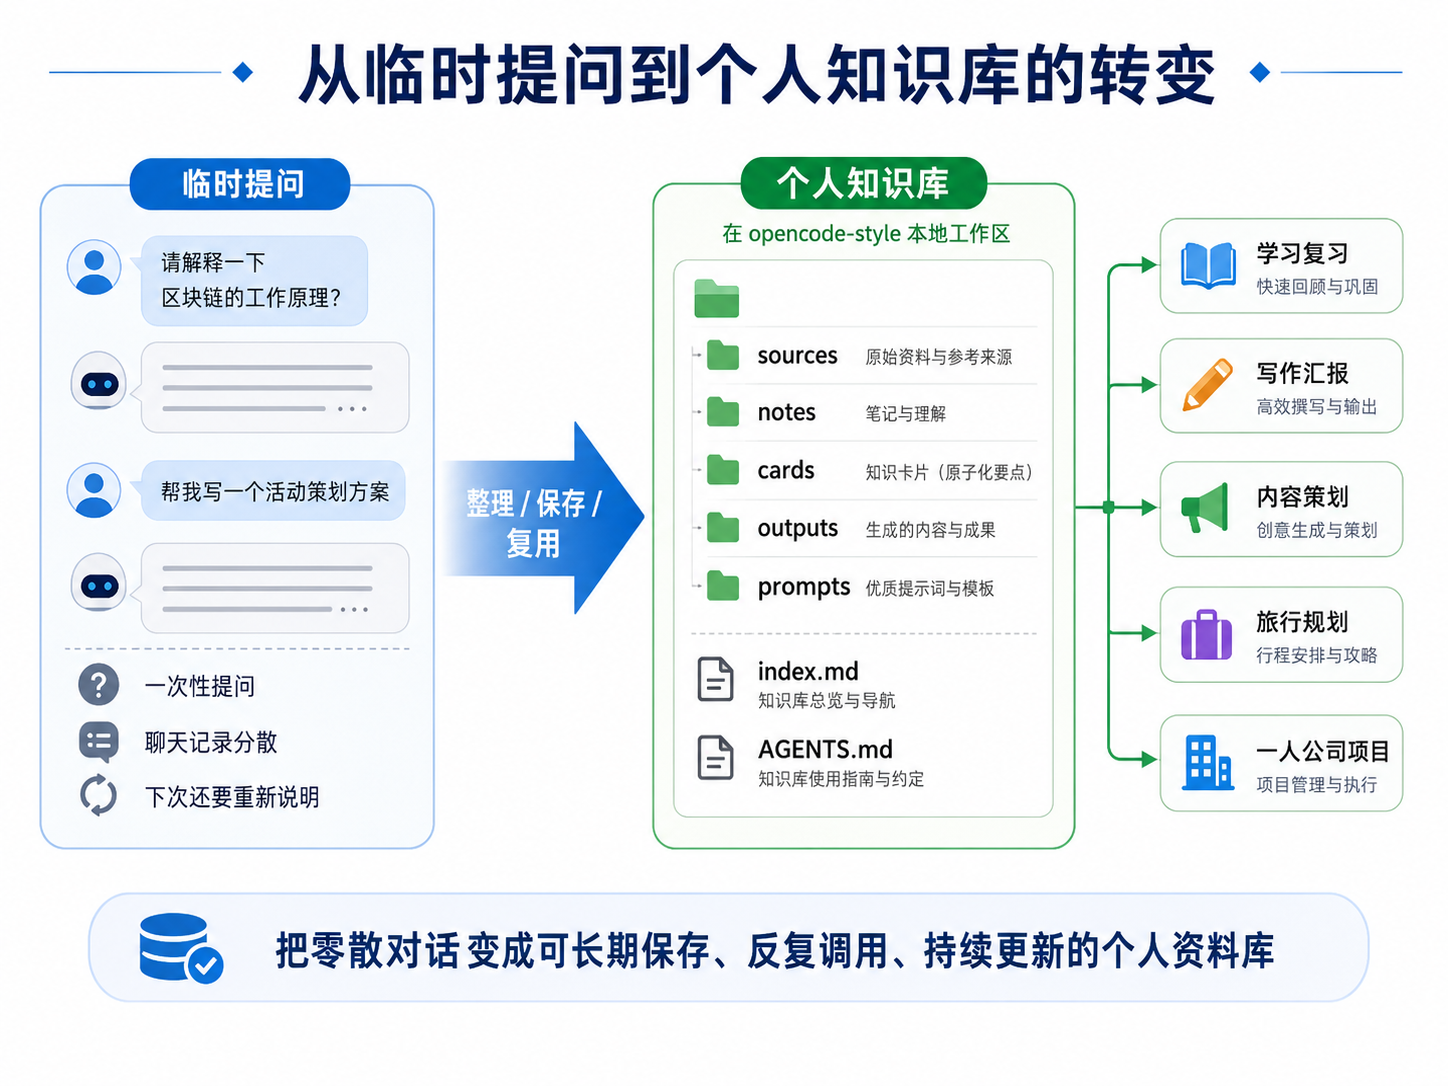
\includegraphics[width=0.88\textwidth]{images_8/个人知识库.png}
    \caption{从临时提问到个人知识库的转变}
    \label{fig:ask-to-knowledge-base}
\end{figure}
\FloatBarrier

\minorheading{最终效果：先看知识库长什么样}

搭建完成后，个人知识库不是一个复杂系统，而是一个结构清楚的本地文件夹。这个文件夹中既保存原始资料，也保存资料卡、索引、提示词和输出成果。一个最小可用的知识库可以采用下面的结构：

\begin{tcolorbox}[filebox,title=个人知识库目录结构]
\begin{verbatim}
my-knowledge-base
├── sources    原始资料
├── notes      学习笔记
├── cards      资料卡
├── outputs    生成成果
├── prompts    提示词和 Skill
├── index.md   总索引
└── AGENTS.md  opencode 工作规则
\end{verbatim}
\end{tcolorbox}

其中，\texttt{sources} 用来保存原始资料，例如文章、课堂资料、网页摘录、合同样本、技术文档等；\texttt{notes} 用来保存自己的学习笔记；\texttt{cards} 用来保存资料卡；\texttt{outputs} 用来保存 AI 辅助生成的复习提纲、脚本、方案等成果；\texttt{prompts} 用来保存常用提示词和 Skill；\texttt{index.md} 是知识库总索引；\texttt{AGENTS.md} 是写给 \texttt{opencode} 的工作规则。











   
\minorheading{创建文件夹：建立固定资料空间}

先在电脑中建立一个专门保存资料的文件夹。为了减少路径识别问题，文件夹名称建议使用英文，文件夹里的正文内容可以正常写中文。

\begin{tcolorbox}[stepbox,title=操作 1：手动创建文件夹]
打开电脑中的“文档”目录，新建一个文件夹，命名为：

\begin{verbatim}
my-knowledge-base
\end{verbatim}

然后进入这个文件夹，继续新建五个子文件夹：

\begin{verbatim}
sources
notes
cards
outputs
prompts
\end{verbatim}
\end{tcolorbox}

如果熟悉终端，也可以使用下面的命令一次性创建：

\begin{tcolorbox}[filebox,title=可选：终端命令]
\begin{verbatim}
cd ~/Documents
mkdir -p my-knowledge-base
cd my-knowledge-base
mkdir -p sources notes cards outputs prompts
\end{verbatim}
\end{tcolorbox}

这一步完成后，知识库的基本容器就建好了。接下来要做的，是告诉 \texttt{opencode}：这个文件夹不是普通代码项目，而是一个个人知识库。

\minorheading{创建规则：写好 AGENTS.md}

\texttt{AGENTS.md} 可以理解为写给 \texttt{opencode} 的“工作说明书”。它告诉 AI：回答问题前应该先看哪些文件，哪些资料不能随便修改，哪些内容不能编造，哪些结果需要人工核验。

\begin{tcolorbox}[stepbox,title=操作 2：创建工作规则文件]
在 \texttt{my-knowledge-base} 文件夹中新建一个文件，命名为：

\begin{verbatim}
AGENTS.md
\end{verbatim}

然后把下面的内容写进去。
\end{tcolorbox}

\begin{tcolorbox}[filebox,title=AGENTS.md 示例]
你是我的个人知识库助手。这个文件夹不是代码项目，而是学习和创作资料库。

工作规则：

1. 回答问题前，优先查看 index.md，再根据索引读取 sources、notes、cards 中的相关文件。

2. 回答必须说明依据来自哪个文件；如果资料中没有依据，要明确说“知识库中暂未找到依据”。

3. 不要编造来源、价格、时间、政策、法律、医疗、金融结论。

4. sources 文件夹保存原始资料，除非明确要求，不要修改。

5. notes 文件夹保存学习笔记，可以根据需要整理，但不要删除原意。

6. cards 文件夹保存资料卡，资料卡应包含来源、主题、摘要、关键词、适用场景、可提问问题和需要核验的信息。

7. outputs 文件夹保存生成成果，例如复习提纲、短视频脚本、汇报稿和内容方案。

8. prompts 文件夹保存可复用提示词和 Skill。

9. 涉及法律、金融、医疗、合同、隐私、版权和公开发布的内容，必须提醒人工核验。
\end{tcolorbox}

有了这个文件，\texttt{opencode} 在这个目录中工作时，就有了明确规则。它不应该直接凭空回答，而应先查看索引和相关资料，再给出整理结果。

\minorheading{创建索引：写好 index.md}

\texttt{index.md} 是个人知识库的总索引。它的作用类似一本书的目录：记录每份资料放在哪里、来自哪里、讲什么、以后可以回答哪些问题。没有索引，资料再多也只是堆在一起；有了索引，AI 才能更快找到应该读取的材料。

\begin{tcolorbox}[stepbox,title=操作 3：创建知识库总索引]
在 \texttt{my-knowledge-base} 文件夹中新建一个文件，命名为：

\begin{verbatim}
index.md
\end{verbatim}

然后写入下面的索引模板。
\end{tcolorbox}

\begin{tcolorbox}[filebox,title=index.md 示例]
\# 个人知识库索引

\#\# 资料登记表

| 编号 | 文件路径 | 来源/日期 | 主题 | 一句话摘要 | 标签 | 可以问的问题 | 需要核验 |
|---|---|---|---|---|---|---|---|

\#\# 使用规则

1. 回答问题前，先查看本索引。

2. 根据主题和标签找到相关 sources、notes 或 cards 文件。

3. 如果资料不足，要说明“知识库中暂未找到依据”。

4. 涉及事实、价格、政策、法律、金融、医疗、版权和公开发布内容，必须标注“需要人工核验”。
\end{tcolorbox}

以后每加入一份新资料，都要在 \texttt{index.md} 中登记。这样做看起来多了一步，但后面复习、写作、查询资料时会省很多时间。

\minorheading{放入资料：保存第一份原始材料}

第一次练习时，不建议直接放很长的 PDF 或大量图片。可以先放一段较短的文字资料，比如课堂笔记、文章摘要，或者前面整理过的“AI 学习方法”内容。这样更容易观察 \texttt{opencode} 如何读取、整理和生成资料卡。

\begin{tcolorbox}[stepbox,title=操作 4：保存第一份资料]
在 \texttt{sources} 文件夹中新建一个文件，命名为：

\begin{verbatim}
2026-05-ai-learning.md
\end{verbatim}

文件名中可以包含日期和主题，方便以后查找。不要使用“资料1”“最终版”“新建文档”这类名称。
\end{tcolorbox}

可以在文件中写入下面这段示例资料：

\begin{tcolorbox}[filebox,title=sources/2026-05-ai-learning.md 示例]
\# AI 学习方法笔记

来源：课堂整理

日期：2026 年 5 月

内容摘要：

AI 可以辅助解释概念、拆解资料、生成练习和整理复习提纲。但使用 AI 学习时，不能只复制答案，而要检查自己是否能够用自己的话解释概念、举出例子、完成类似练习，并把重要资料整理进个人知识库。
\end{tcolorbox}

这一步完成后，知识库里就有了第一份原始资料。接下来可以让 \texttt{opencode} 基于这份资料生成资料卡。

\minorheading{生成卡片：让 opencode 提炼资料卡}

资料卡相当于一份资料的“压缩说明”。它不是全文复制，而是提炼资料来源、主题、核心观点、关键词、可提问问题和需要核验的信息。以后查询知识库时，\texttt{opencode} 可以先看资料卡，再决定是否需要打开原始资料。

\begin{tcolorbox}[stepbox,title=操作 5：进入知识库并启动 opencode]
打开终端，进入刚才创建的知识库文件夹：

\begin{verbatim}
cd ~/Documents/my-knowledge-base
opencode
\end{verbatim}

如果不熟悉终端，可以先打开 \texttt{opencode}，再把当前工作目录切换到 \texttt{my-knowledge-base}。关键是让 \texttt{opencode} 在这个知识库文件夹中工作。
\end{tcolorbox}

进入 \texttt{opencode} 后，可以输入：

\begin{tcolorbox}[filebox,title=提示词或示例内容]
请阅读 @sources/2026-05-ai-learning.md，并为它生成一张资料卡。资料卡保存到 cards/2026-05-ai-learning-card.md。

资料卡必须包括：资料来源、主题、适合解决的问题、核心观点、关键词、可复习问题、需要人工核验的信息。

不要添加资料中没有出现的内容。
\end{tcolorbox}

这里的 \texttt{@sources/2026-05-ai-learning.md} 表示引用知识库中的某个文件。如果工具支持文件选择，输入 \texttt{@} 后可以按提示选择对应文件。

资料卡生成后，要打开检查一遍。重点看三点：有没有添加资料中没有的内容；有没有把不确定信息写成确定结论；关键词和可提问问题是否方便以后检索。

\minorheading{更新索引：把资料登记进目录}

资料卡生成后，还要把这份资料登记到 \texttt{index.md}。如果只生成资料卡而不更新索引，资料仍然会逐渐散掉。索引更新以后，后面提问时 \texttt{opencode} 才能先通过目录找到相关内容。

\begin{tcolorbox}[stepbox,title=操作 6：更新知识库索引]
在 \texttt{opencode} 中继续输入下面的指令，让它根据资料卡更新总索引。
\end{tcolorbox}

\begin{tcolorbox}[filebox,title=提示词或示例内容]
请根据 @cards/2026-05-ai-learning-card.md，更新 @index.md 的“资料登记表”。

新增一行，填写文件路径、来源/日期、主题、一句话摘要、标签、可以问的问题和需要核验的内容。

只更新索引，不要修改 sources 中的原始资料。
\end{tcolorbox}

更新完成后，要打开 \texttt{index.md} 看一眼：文件路径是否正确，摘要是否准确，标签是否便于以后查找，是否把不确定内容写成了确定结论。这个人工检查步骤不能省略。
\minorheading{开始提问：让 opencode 基于资料回答}

当知识库中至少有一份原始资料、一张资料卡和一个索引后，就可以开始提问。此时的关键是：不要只问“帮我总结一下”，而要明确要求 \texttt{opencode} 先查知识库，再根据资料回答，并说明依据来自哪个文件。

\begin{tcolorbox}[stepbox,title=操作 7：基于知识库提问]
在 \texttt{opencode} 中输入下面的指令，测试知识库是否能够被调用。
\end{tcolorbox}

\begin{tcolorbox}[filebox,title=提示词或示例内容]
请先查看 @index.md，再根据知识库中的资料回答：我现在想复习 AI 学习方法，哪些资料最相关？请列出依据文件，并说明每份资料适合解决什么问题。
\end{tcolorbox}

也可以继续输入：

\begin{tcolorbox}[filebox,title=提示词或示例内容]
请基于我的个人知识库，帮我整理一份“AI 辅助学习”的复习提纲。要求说明依据来自哪些 cards 或 sources 文件。如果知识库中没有依据，请明确说明，不要凭空补充。
\end{tcolorbox}

如果以后知识库中加入了家乡旅游、短视频脚本、出行准备、菜单翻译、资料整理等内容，也可以让 \texttt{opencode} 基于这些已有资料继续生成新的成果。例如：

\begin{tcolorbox}[filebox,title=提示词或示例内容]
请基于我的知识库，查找与“家乡旅游宣传素材”有关的资料，并帮我整理可用素材、可生成内容和需要人工核验的信息。
\end{tcolorbox}

这样，知识库就不只是保存资料，而是可以被调用、被追问、被复用。
\minorheading{保存提示词：沉淀常用流程}

如果经常让 \texttt{opencode} 做同一类事情，就可以把提示词保存到 \texttt{prompts} 文件夹中。这样以后不必每次重新写完整指令，只需要打开对应提示词，再替换文件名或任务主题即可。

\begin{tcolorbox}[stepbox,title=操作 8：保存资料卡生成提示词]
在 \texttt{prompts} 文件夹中新建一个文件，命名为：

\begin{verbatim}
make-card.md
\end{verbatim}

然后写入下面内容。
\end{tcolorbox}

\begin{tcolorbox}[filebox,title=prompts/make-card.md 示例]
请阅读用户指定的 sources 文件，并生成资料卡。

资料卡保存到 cards 文件夹。

资料卡必须包括：

1. 资料来源

2. 主题

3. 适合解决的问题

4. 核心观点

5. 关键词

6. 可复习问题

7. 需要人工核验的信息

要求：

- 不添加资料中没有出现的内容。

- 不确定内容标注“需要核验”。

- 不修改 sources 中的原始资料。
\end{tcolorbox}

以后需要生成资料卡时，就可以让 \texttt{opencode} 读取这份提示词，再补充具体文件名。常用流程还可以继续整理成 Skill，例如“资料卡生成助手”“知识库索引更新助手”“学习资料整理助手”。

\begin{figure}[H]
    \centering
    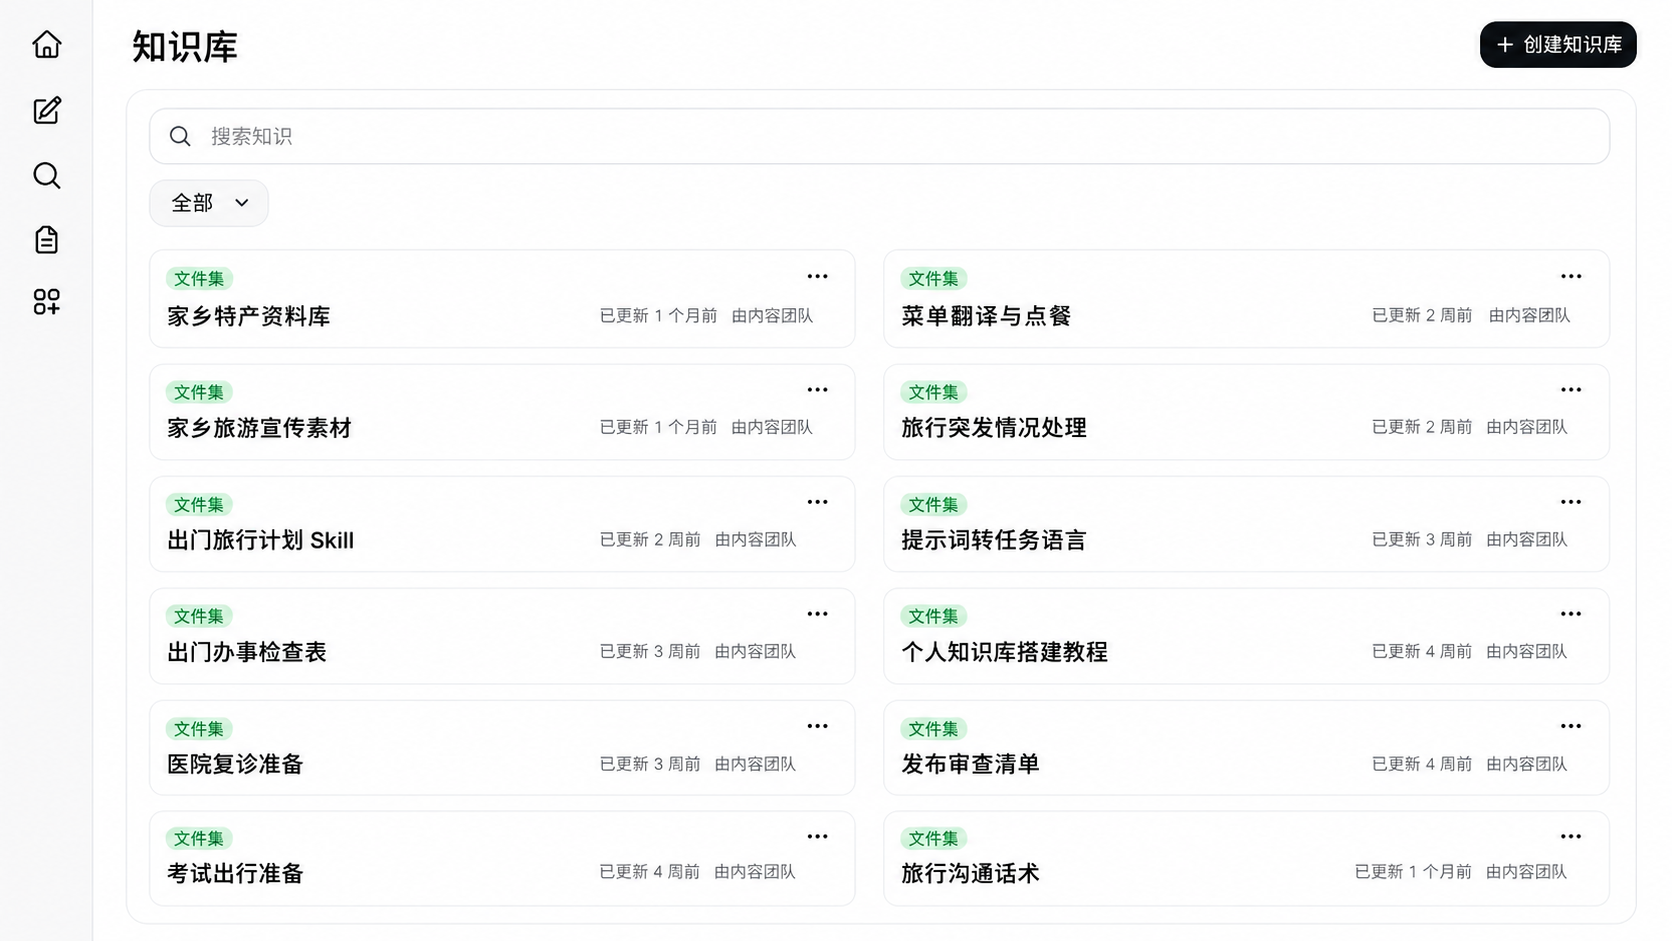
\includegraphics[width=0.88\linewidth]{ChatGPT Image 2026年5月27日 16_51_10.png}
    \caption{个人知识库展示}
    \label{fig:placeholder}
\end{figure}

\minorheading{安全边界：保护隐私与敏感资料}

个人知识库搭好以后，可以按照固定流程使用：

\begin{tcolorbox}[filebox,title=个人知识库日常流程]
\begin{verbatim}
新资料进入 sources
        ↓
生成资料卡到 cards
        ↓
更新 index.md
        ↓
基于知识库提问
        ↓
有价值的输出保存到 outputs
        ↓
常用提示词保存到 prompts
\end{verbatim}
\end{tcolorbox}

比如，今天保存了一篇关于 AI 学习方法的文章，明天可以让 \texttt{opencode} 生成资料卡并更新索引；后天要写学习总结时，就可以让 \texttt{opencode} 先查索引，再基于资料卡生成提纲。这样，学习不再是一次次零散提问，而是逐步形成一个可以积累、查询和复用的个人知识系统。

\begin{tcolorbox}[warnbox]
个人知识库越用越久，里面可能会保存证件号码、手机号、家庭住址、订单截图、合同内容、客户资料、公司文件等敏感信息。放入知识库前，应先判断是否需要脱敏。涉及身份证、护照、银行卡、验证码、病历、合同敏感条款、客户名单和未公开项目资料时，不要直接原样放入。涉及法律、金融、医疗、合同、版权和公开发布的内容，知识库只能辅助理解和整理，不能替代专业判断。
\end{tcolorbox}

个人知识库的价值，不在于文件数量有多少，而在于资料是否清楚、来源是否可靠、索引是否好用、能否被 AI 正确调用。以后无论是学习复习、写作汇报、制作家乡旅游宣传视频，还是继续搭建更复杂的个人智能体，都可以在这个知识库基础上扩展。
% ====================== 8.4 ======================


% ============================================================
% 8.4 求职沟通与简历优化
% ============================================================

\section{工作协作与职业发展}

\subsection{履历呈现与自我展示}

过去谈到简历，很多人会觉得它只是“把自己的经历写清楚”。但在 AI 已经进入招聘流程之后，简历不再只是写给人看的材料，也可能会先被算法读取、筛选和排序。换句话说，求职者不仅要让招聘者看懂自己，也要让招聘系统更准确地识别自己的经历与岗位之间的匹配关系。

《AI Self-preferencing in Algorithmic Hiring》这项研究就提出了一个值得注意的现象：当求职者使用 AI 修改简历，而企业也使用大语言模型筛选简历时，招聘模型可能更偏好 AI 生成或同类模型生成的简历。研究者在模拟招聘流程中发现，在资质相同的情况下，使用同类大语言模型修改简历的候选人，进入候选名单的概率比提交人工简历的候选人高 23\%—60\%。这说明，AI 辅助求职已经不只是“润色几句话”，还涉及简历表达风格、岗位关键词、平台筛选机制和算法偏好的适配问题。

\begin{figure}[H]
    \centering
    
\includegraphics[width=0.88\textwidth]{\detokenize{images_8/当AI招聘遇上AI简历_系统性的偏好.png}}
    \caption{当 AI 招聘遇上 AI 简历：系统性的偏好}
    \label{fig:ai-hiring-preference}
\end{figure}

这并不是鼓励读者用 AI 编造经历，而是提醒大家：在新的求职环境中，真实经历也需要被更清楚、更结构化地表达出来。如果简历只是写“参与活动”“负责沟通”“完成项目”，招聘者和系统都很难判断你的真实能力；如果能写清楚任务背景、本人职责、使用方法和实际结果，简历就会更容易被理解。AI 的正确作用，是帮助读者把真实经历整理成更准确、更有岗位匹配度的表达，而不是把没有做过的事情包装成经历。

\subsubsection*{先读懂岗位，再开始写简历}

很多人使用 AI 写简历时，一上来就输入：“帮我写一份简历。”这种做法通常效果不好。因为简历不是孤立存在的，它必须和目标岗位相匹配。同样一段经历，投新媒体运营、行政助理、教师助理、Java 开发、销售岗位时，应该突出完全不同的能力。

求职准备的第一步，是把岗位要求读懂。读者可以把招聘信息提供给 AI，然后输入：

\begin{tcolorbox}[promptbox]
请帮我分析这份岗位要求。请提取岗位核心职责、必须具备的能力、加分项、简历中应该重点体现的关键词，以及面试时可能被追问的问题。请用表格输出，并区分“必须体现”和“可以加分”的内容。
\end{tcolorbox}

例如，一份岗位要求中写着“负责活动策划与执行、社群维护、用户反馈整理、基础数据统计”，AI 就可以帮助读者拆出几个核心能力：活动执行能力、沟通协调能力、信息整理能力、数据意识和用户服务意识。这样，后面修改简历时，就不再是泛泛地写“本人沟通能力强”，而是要用真实经历证明这些能力。

英国 National Careers Service 在简历建议中也强调，简历应当根据申请岗位进行调整，结合岗位说明、必要条件和公司信息来匹配内容，同时更新新的成就、经历和技能，删除过时信息。 这说明，简历不是一份材料投所有岗位，而是要根据岗位不断调整重点。

\subsubsection*{把自己的经历整理成可用素材}

读懂岗位以后，第二步是整理自己的经历。很多读者觉得自己“没什么可写”，其实往往不是没有经历，而是没有把经历拆开。一次课程项目、社团活动、志愿服务、实习任务、兼职经历、比赛作品、公众号运营、毕业设计，都可能包含可以写进简历的内容。

整理经历时，可以让 AI 帮忙搭一个表格。输入：

\begin{tcolorbox}[promptbox]
我准备申请【岗位名称】。下面是我做过的一些真实事情，请帮我判断哪些经历适合写进简历，并整理成“任务背景—我负责什么—使用了什么方法—形成了什么结果—对应岗位能力”的表格。注意：只能基于我提供的信息，不要编造数据和经历。
\end{tcolorbox}

然后补充真实经历，例如：

\begin{tcolorbox}[promptbox]
我参加过学院迎新活动，负责新生群通知、报名表收集和现场签到。
我做过课程小组作业，负责资料整理和 PPT 制作。
我运营过班级公众号，写过 5 篇推文。
我会用 Excel 做简单统计，也会用剪映剪视频。
\end{tcolorbox}

AI 可以帮助读者发现，这些经历并不是“没什么可写”。“负责新生群通知”可以体现信息传达和社群沟通；“报名表收集”可以体现资料整理和表格处理；“现场签到”可以体现活动执行和现场协调；“公众号推文”可以体现内容写作和平台运营。经过整理以后，原本零散的经历就能变成简历素材。

\begin{figure}[H]
    \centering
    
\includegraphics[width=0.88\textwidth]{\detokenize{images_8/简历经历整理_AI界面示例.png}}
    \caption{AI 辅助整理简历经历匹配表格示例}
    \label{fig:resume-experience-match}
\end{figure}

这里要注意，AI 可以帮助挖掘真实经历中的价值，但不能虚构没有发生过的内容。如果没有负责数据分析，就不能写成“独立完成数据分析”；如果只是参与活动，就不能写成“主导活动策划”；如果没有统计结果，就不能让 AI 编造“提升 50\%”“覆盖 1000 人”“转化率显著提高”。简历是面试时会被追问的材料，真实性比漂亮表达更重要。

\subsubsection*{把经历改写成简历语言}

简历语言不需要华丽，但要具体、清楚、能证明能力。比较实用的写法是：动作 + 任务 + 方法 + 结果。如果有真实数据，可以写数据；如果没有数据，也可以写清楚完成了什么产出、服务了什么对象、承担了什么职责。

普通写法：
\begin{quote}
参与学校迎新活动。
\end{quote}

优化后：
\begin{quote}
参与学院迎新活动，负责新生群通知、报名信息收集和现场签到协助，帮助新生完成报到流程。
\end{quote}

如果有真实数据，可以进一步写成：
\begin{quote}
参与学院迎新活动，负责 3 个新生群的信息通知、报名表收集和现场签到协助，整理 300 余条报名信息，帮助新生顺利完成报到流程。
\end{quote}

这两种写法都没有编造经历，但第二种更具体，第三种在有真实数据的情况下更有说服力。AI 可以帮助读者把“我做过什么”改成“这件事体现了什么能力”。

可以输入：

\begin{tcolorbox}[promptbox]
请帮我把下面这段经历改写成适合简历的表达。要求：语言简洁，突出我负责的工作、使用的方法和体现的能力；如果没有明确数据，不要编造，请提醒我哪些地方可以补充真实数据。
原始经历：【粘贴经历】
\end{tcolorbox}

AI 输出后，读者要逐句检查。凡是出现“主导”“统筹”“独立负责”“显著提升”“大幅增长”等词，都要确认是否符合真实情况。如果自己只是协助，就写“协助”；如果只是参与，就写“参与”；如果确实负责某个模块，再写“负责”。简历表达可以优化，但职责边界不能随意升级。

\subsubsection*{根据不同岗位定制简历重点}

同一份基础简历，不适合直接投所有岗位。比如，一个学生有“活动组织、公众号运营、课程项目、Excel 统计”几类经历。投新媒体运营时，应重点写公众号、文案、选题、平台发布和数据反馈；投行政助理时，应重点写材料整理、活动协调、表格统计、流程执行；投销售助理时，应重点写客户沟通、信息记录、问题反馈和跟进意识。

这时可以让 AI 做岗位匹配分析：

\begin{tcolorbox}[promptbox]
我有一份基础简历和一个目标岗位 JD。请帮我做岗位匹配分析：
这个岗位最看重哪些能力；
我的简历中哪些内容最匹配；
哪些经历应该放在更靠前的位置；
哪些表达需要改得更具体；
哪些内容与岗位关系不大，可以弱化。
注意：不要编造经历，只能基于我提供的材料提出修改建议。
\end{tcolorbox}

AI 的价值在于帮助读者“重新排序”和“突出重点”。它不是简单把简历写长，而是帮助判断：哪些经历最应该放在前面，哪些关键词应该出现，哪些内容可以删减。LinkedIn 工程博客介绍，其 AI-powered job search 已经允许用户用自然语言描述想找的工作，并根据理想岗位返回更匹配的结果，这也说明求职正在从传统关键词匹配，逐渐走向更强的语义匹配和意图理解。

因此，读者在修改简历时，也要学会从“堆关键词”转向“表达匹配关系”。岗位要求“活动执行”，简历中就要有真实活动经历；岗位要求“数据整理”，简历中就要体现表格、统计、整理和反馈；岗位要求“客户沟通”，简历中就要体现沟通对象、沟通内容和处理结果。

\subsubsection*{写好个人总结和求职信}

很多简历开头会有“个人总结”或“求职意向”。这部分不能写成空泛评价，例如“本人性格开朗、吃苦耐劳、学习能力强”。更好的写法是用两三句话说明自己的背景、目标岗位和最相关优势。

可以让 AI 帮助生成个人总结：

\begin{tcolorbox}[promptbox]
请根据我的经历和目标岗位，帮我写一段 80 字以内的简历个人总结。要求：突出与岗位最相关的 2—3 个能力，不要写空话，不要使用“吃苦耐劳、认真负责”这类泛泛表达。
\end{tcolorbox}

如果申请场景需要求职信，也可以输入：

\begin{tcolorbox}[promptbox]
我准备申请【岗位名称】，下面是岗位要求和我的经历。请帮我生成一版 300 字以内的求职信初稿。内容包括：我为什么申请这个岗位、我有哪些相关经历、我能为团队带来什么。语气正式但自然，不要夸张，不要编造经历。
\end{tcolorbox}

求职信不是重复简历，而是把“岗位需求”和“个人经历”连接起来。例如，可以写自己为什么对这个方向感兴趣，过去哪段经历与岗位相关，自己希望如何在岗位中继续发挥作用。AI 可以生成初稿，但最终要改成自己的语言，避免所有人都写出相似的 AI 味表达。

\subsubsection*{准备面试自我介绍}

简历通过筛选后，面试通常会先要求自我介绍。很多读者的自我介绍容易出现两个问题：一种是太短，只说姓名、学校、专业；另一种是太长，把简历从头到尾背一遍。更合适的自我介绍应该围绕目标岗位展开，一般包括三个部分：基本背景、相关经历、岗位兴趣。

可以输入：

\begin{tcolorbox}[promptbox]
请根据我的简历和目标岗位，帮我准备一段 1 分钟中文自我介绍。要求：先说明我的背景，再突出 2 个与岗位最相关的经历，最后表达我对岗位的兴趣。语言自然，不要像背稿。
\end{tcolorbox}

AI 生成后，还可以继续优化：

\begin{tcolorbox}[promptbox]
这版自我介绍有点书面化，请改成更适合面试现场说出来的版本，句子短一点，语气自然一点，不要使用夸张词。
\end{tcolorbox}

准备自我介绍时，读者要注意两点。第一，不要把所有经历都塞进去，只讲和岗位最相关的经历。第二，不要背诵 AI 生成稿，而要理解结构后用自己的话表达。面试官更希望听到真实、清楚、有重点的表达，而不是一段过度包装的标准答案。

\subsubsection*{用 AI 做面试问题预测和模拟练习}

AI 在面试准备中很有用。它可以根据岗位要求和简历内容，预测面试官可能会问什么问题，也可以根据读者的回答给出修改建议。

可以输入：

\begin{tcolorbox}[promptbox]
请根据我的简历和目标岗位，帮我预测 10 个面试问题。请分成三类：岗位能力问题、项目经历追问、综合素质问题。每个问题后面说明面试官想考察什么，以及我应该用哪段经历回答。
\end{tcolorbox}

常见问题包括：
\begin{itemize}
    \item 你为什么申请这个岗位？
    \item 你最能体现沟通能力的一段经历是什么？
    \item 你在项目中遇到过什么困难？怎么解决？
    \item 如果临时任务很多，你会如何安排优先级？
    \item 你对这个岗位的理解是什么？
\end{itemize}

回答经历类问题时，可以用“情境—任务—行动—结果”的结构。也就是先说当时是什么情况，再说自己负责什么，接着说采取了什么行动，最后说结果如何、学到了什么。

\begin{figure}[H]
    \centering
    
\includegraphics[width=0.88\textwidth]{\detokenize{images_8/面试问题预测_AI界面示例.png}}
    \caption{AI 辅助预测面试问题并分类示例}
    \label{fig:interview-question-prediction}
\end{figure}

可以输入：

\begin{tcolorbox}[promptbox]
请用“情境—任务—行动—结果”的结构，帮我整理下面这个经历，变成适合面试回答的版本。要求真实、简洁、口语化，不要编造数据。
经历：【粘贴经历】
\end{tcolorbox}

还可以让 AI 扮演面试官：

\begin{tcolorbox}[promptbox]
请你扮演面试官，针对我申请的【岗位名称】进行模拟面试。一次只问一个问题。等我回答后，请从内容完整性、表达清晰度、岗位匹配度三个方面给我反馈，并提出修改建议。
\end{tcolorbox}

这种练习的意义，不是背出完美答案，而是发现自己的表达问题。比如回答是否太空、是否没有说结果、是否没有体现岗位能力、是否回答偏题。经过几轮练习后，读者会更清楚自己应该讲哪段经历、怎么讲、讲到什么程度。

\subsubsection*{检查 AI 生成内容中的风险}

AI 可以提高求职准备效率，但也可能带来风险。最常见的问题是：表达过度包装，经历被夸大，数据被编造，职责被升级，关键词被堆砌。简历看起来更强了，但面试时解释不了，反而会降低信任。

使用 AI 优化简历后，读者要逐项检查：
\begin{itemize}
    \item 第一，经历是否真实。自己没有做过的内容必须删除。
    \item 第二，职责是否准确。参与、协助、负责、主导，不能混用。
    \item 第三，数据是否可靠。没有统计过的数据不能编造。
    \item 第四，技能是否掌握。不会的工具、语言、平台不能写成熟练。
    \item 第五，表达是否能解释。简历上每一句话，都要能在面试中讲清楚。
\end{itemize}

还要注意隐私保护。上传简历给 AI 前，可以隐藏身份证号、详细住址、完整手机号、证件号码、公司内部资料、未公开项目数据等敏感信息。AI 可以帮你修改表达，但不需要知道所有个人隐私。




\subsection{会议协作：会前准备、会中记录与会议纪要}

很多人一听到“开会”，第一反应就是“坐在那里听别人说话”。但真正进入学习、实习和工作以后就会发现，会议并不是简单地把人聚在一起，而是一个非常典型的协作场景。一次会议如果准备不好，就容易变成大家各说各的；记录不好，开完以后谁也记不清刚才到底定了什么；纪要写不好，就会出现“会上好像说过”“我以为不是我负责”“这个时间不是下周吗”之类的问题。

AI 在会议场景中的价值，正是帮助我们把会议从“说过了”变成“说清楚了”，再进一步变成“可以执行了”。现在许多办公工具已经把 AI 会议能力做进产品中。例如，Microsoft Teams 中的 Copilot 可以总结会议讨论重点，说明谁说了什么，并建议行动项；Google Meet 中的 Gemini “Take notes for me” 可以捕捉会议笔记和行动项，并生成 Google Docs 文档；Zoom AI Companion 也支持生成会议摘要和后续步骤，并在会议结束后发送摘要。 这些功能说明，AI 会议助手已经不再是概念，而是在真实办公场景中帮助人们减少漏记、整理重点和推进协作。

% \begin{figure}[H]
%     \centering
%     \includegraphics[width=0.88\textwidth]{\detokenize{AI会议协作流程示意图.png}}
%     \caption{AI 会议协作：从语音到可执行结果的流程}
%     \label{fig:meeting-collaboration-flow}
% \end{figure}

不过，会议使用 AI 不能只理解成“开完会自动生成纪要”。一场真正有效的会议，通常包括三个阶段：会前准备、会中记录、会后纪要。本小节重点学习这三个阶段如何使用 AI，让会议更有方向、更有记录、更有结果。

\subsubsection*{会前准备：先把“为什么开会”说清楚}

很多低效会议的问题，其实在会议开始前就已经埋下了。比如会议通知只写“明天下午开会讨论活动方案”，但没有说明讨论什么、需要谁准备材料、会议要形成什么结果。到了会议现场，大家只能临时回忆：活动预算是多少？场地定了吗？谁负责宣传？这次到底是讨论方案，还是拍板决定？这样一来，会议很容易越开越散。

会前使用 AI 的第一步，是让它帮助我们整理会议目标。会议目标不是“开个会”，而是要回答三个问题：这次会议为什么开？需要讨论哪些问题？会议结束时希望得到什么结果？如果这三个问题不清楚，再先进的 AI 会议工具也只能记录一堆散乱发言。

例如，准备一次“校园活动策划会”时，可以这样输入：

\begin{tcolorbox}[promptbox]
我准备组织一次校园活动策划会议。已知活动主题是“AI 学习分享会”，参会人员包括活动负责人、宣传同学、场地对接同学和主持人。请帮我整理会前准备内容，包括会议目标、建议议题、每个议题需要提前准备的材料，以及会议结束时应该形成哪些结论。
\end{tcolorbox}

AI 可以帮助生成一份会前提纲，比如：

\begin{table}[H]
\centering
\caption{校园活动策划会会前提纲}
\label{tab:meeting-pre-outline}
\begin{tabular}{p{0.25\linewidth} p{0.65\linewidth}}
\toprule
\textbf{模块} & \textbf{内容} \\
\midrule
会议目标 & 明确活动时间、地点、宣传方式、人员分工和后续时间表 \\
议题一 & 活动主题和目标受众是否明确 \\
议题二 & 场地、设备和时间是否可行 \\
议题三 & 宣传渠道、推文发布时间和报名方式 \\
议题四 & 主持人、嘉宾、签到、摄影等分工 \\
会议产出 & 活动方案定稿、任务分工表、截止时间和下一次确认节点 \\
\bottomrule
\end{tabular}
\end{table}

这样的会前准备，比只写一句“讨论活动方案”更有效。它让参会者提前知道会议要解决什么问题，也让会议主持人知道应该按什么顺序推进。

如果是项目组会议，也可以输入：

\begin{tcolorbox}[promptbox]
我们明天要开项目进度会，项目是【项目名称】。请帮我设计一份会议议程，要求包括：当前进展汇报、遇到的问题、需要协调的资源、下一阶段任务和风险提醒。请输出一份适合发给参会人员的会前通知。
\end{tcolorbox}

AI 可以生成更完整的会议通知：

\begin{quote}
各位好，明天下午 3 点召开项目进度会。本次会议主要确认当前进展、存在问题和下一阶段任务安排。请各负责人提前准备以下内容：已完成事项、未完成事项、遇到的困难、需要其他成员配合的部分，以及下周计划。会议结束时将形成任务分工表和截止时间。
\end{quote}

这类内容看起来简单，但能大幅减少会议中的无效沟通。因为每个人都知道自己需要带着什么信息来开会。

\subsubsection*{会前材料整理：让 AI 帮你先读一遍资料}

有些会议不是从零开始讨论，而是基于已有材料继续推进，比如项目文档、调研报告、用户反馈、活动方案、会议记录、客户需求清单等。如果参会者没有提前读材料，会议就会变成“现场读文档”。AI 可以帮助我们在会前快速整理材料，提炼重点问题。

可以把会议材料提供给 AI，然后输入：

\begin{tcolorbox}[promptbox]
请阅读这份会议材料，帮我整理会前速读笔记。请包括：材料主要内容、已经明确的结论、仍然不清楚的问题、会议中需要重点讨论的事项，以及我应该提前准备的发言要点。
\end{tcolorbox}

\begin{figure}[H]
    \centering
    
\includegraphics[width=0.88\textwidth]{\detokenize{images_8/会前材料整理_AI界面示例.png}}
    \caption{AI 辅助整理会议材料重点与待讨论事项示例}
    \label{fig:pre-meeting-material-sort}
\end{figure}

AI 输出后，读者可以重点看两类内容：一类是“已经明确的信息”，比如活动时间、项目目标、客户需求；另一类是“仍然需要讨论的信息”，比如预算没确定、负责人没明确、风险没有处理方案。这样，会议就不会浪费大量时间重复已经清楚的内容，而是把时间留给真正需要讨论的问题。

如果是学生小组作业，也可以这样使用：

\begin{tcolorbox}[promptbox]
下面是我们小组目前的作业资料。请帮我整理下一次小组会议要讨论的问题。要求区分：已经完成的部分、需要补充的部分、需要组员共同决定的部分，以及我可以在会上汇报的内容。
\end{tcolorbox}

这样，AI 不只是帮忙总结资料，还能帮读者找到“会上该说什么”。很多人开会时不知道怎么发言，其实不是没有想法，而是没有提前把材料和问题整理出来。

\subsubsection*{会前发言准备：让表达更有条理}

会议中，很多人发言容易出现两种情况：一种是太短，只说“我这边没问题”；另一种是太散，说了很多细节，但别人听不出重点。会前可以让 AI 帮自己准备发言提纲，让表达更清楚。

例如，项目进度汇报可以使用这个提示：

\begin{tcolorbox}[promptbox]
我需要在项目会议上汇报自己的进展。请根据下面的信息帮我整理一段 1 分钟发言。要求包括：已完成事项、当前问题、下一步计划和需要协助的地方。语言自然，适合会议现场表达，不要写得像正式文章。
我的信息是：【粘贴自己的进展记录】
\end{tcolorbox}

AI 可以把零散记录整理成这样的发言：

\begin{quote}
我这边本周主要完成了报名表设计和活动推文初稿，目前报名表已经可以使用，推文还需要补充嘉宾介绍。现在主要问题是嘉宾简介还没有最终确认，所以宣传发布时间可能会受到影响。下一步我会先完善推文结构，同时等嘉宾信息确认后补充内容。需要大家协助的是，负责嘉宾对接的同学最好在明天下午前给我最终版简介。
\end{quote}

这样的发言有四个要素：完成了什么、遇到什么问题、下一步做什么、需要谁协助。它比“我这边还在做推文”更清楚，也更容易让会议产生结果。

如果读者要在客户会议中发言，语气还要更谨慎。可以输入：

\begin{tcolorbox}[promptbox]
请帮我把下面这段内部表达改成适合客户会议的发言。要求：语气专业、不过度承诺，清楚说明目前进展、可交付内容和需要客户确认的问题。
\end{tcolorbox}

这种用法可以帮助读者区分内部沟通和外部沟通。内部会议可以直接说问题，客户会议则要更注意表达方式，既要说明进展，也不能随意承诺无法确认的结果。

\subsubsection*{会中记录：不要只记“谁说了什么”，还要记“会议形成了什么”}

会议开始以后，AI 可以帮助记录，但记录不是把所有话一字不落写下来。真正有用的会议记录，应该能回答几个问题：会议讨论了什么？形成了哪些结论？哪些问题还没解决？谁负责什么？什么时候完成？哪些内容需要会后确认？

现在很多会议工具已经在这方面提供支持。Teams 中的 Copilot 可以在会议中或会后总结讨论重点、回答关于会议内容的问题，并建议行动项；Google Meet 的“Take notes for me”会将会议记录和后续事项组织到文档中，并可附加到日历事件，便于参会者后续访问；Zoom 的 AI Companion Meeting Summary 可以在主持人启用后生成会议摘要，会议结束后发送总结内容。

但在实际学习和工作中，不是每个人都能使用这些高级办公工具。有时只是线下小组会，有时只是普通语音会议，有时只有自己手动记录。即使没有自动会议助手，也可以用 AI 参与会中记录的后半段：先由人记录要点，再让 AI 整理结构。

会中记录时，可以按照下面这个格式记：

\begin{table}[H]
\centering
\caption{会中记录项目}
\label{tab:meeting-record-items}
\begin{tabular}{p{0.25\linewidth} p{0.65\linewidth}}
\toprule
\textbf{记录项目} & \textbf{应记录内容} \\
\midrule
讨论主题 & 这部分在讨论什么问题 \\
主要观点 & 各方提出了哪些看法 \\
已定结论 & 哪些事情已经确定 \\
待确认问题 & 哪些事情还没有确定 \\
任务分工 & 谁负责什么 \\
截止时间 & 什么时候完成 \\
风险提醒 & 可能影响进度的问题 \\
\bottomrule
\end{tabular}
\end{table}

比如，在一次活动策划会上，原始记录可能很乱：
\begin{quote}
宣传要提前发。海报小王负责。报名表还没做好。场地可能要换。老师说周三前要确定嘉宾。主持人还没定。预算要再问一下。
\end{quote}

这段记录虽然有信息，但不适合直接作为纪要。可以会后输入：

\begin{tcolorbox}[promptbox]
请把下面这段会议记录整理成结构化会议纪要。要求包括：会议主题、主要结论、任务分工、截止时间、待确认问题和风险提醒。不要编造没有出现的信息，不能确定的内容标注“待确认”。
原始记录：【粘贴记录】
\end{tcolorbox}

AI 可以整理成：

\begin{table}[H]
\centering
\caption{结构化会议纪要示例}
\label{tab:structured-meeting-minutes-example}
\begin{tabular}{p{0.25\linewidth} p{0.65\linewidth}}
\toprule
\textbf{类别} & \textbf{内容} \\
\midrule
会议主题 & 活动策划推进会 \\
已定事项 & 宣传需要提前发布；海报由小王负责；嘉宾需在周三前确认 \\
待完成任务 & 完成报名表；确认主持人；核实预算；确认场地是否变更 \\
风险提醒 & 场地可能变更，可能影响宣传信息；嘉宾未确认会影响推文发布时间 \\
待确认问题 & 最终场地、预算金额、主持人人选 \\
\bottomrule
\end{tabular}
\end{table}

这样，原本散乱的口头讨论就变成了可以检查的会议记录。

\subsubsection*{会议纪要：把讨论变成可追踪的结果}

会议纪要不是会议录音的文字版，也不是把每个人说过的话全部抄下来。纪要的作用是留下清楚、简洁、可追踪的会议结果。一个好的会议纪要，至少应包括六个部分：会议基本信息、会议主题、主要讨论内容、形成的结论、任务分工、待确认问题。

可以使用这个模板：

\begin{tcolorbox}[promptbox]
请根据下面的会议记录生成会议纪要。
纪要结构包括：
会议名称、时间、参会人员；
会议目标；
主要讨论内容；
已形成的结论；
任务分工表，包括任务、负责人、截止时间；
待确认问题；
下一次会议建议议题。
要求语言正式、简洁，不要编造未提到的信息，责任人和截止时间不明确的地方标注“待确认”。
\end{tcolorbox}

生成后的会议纪要可以这样呈现：

\begin{table}[H]
\centering
\caption{会议纪要模块示例}
\label{tab:meeting-minutes-module-example}
\begin{tabular}{p{0.25\linewidth} p{0.65\linewidth}}
\toprule
\textbf{模块} & \textbf{内容} \\
\midrule
会议名称 & AI 学习分享会筹备会议 \\
会议目标 & 确认活动方案、宣传安排和任务分工 \\
主要结论 & 活动初步定于下周五下午；宣传推文需提前三天发布；报名表本周内完成 \\
任务分工 & 小王负责海报；小李负责报名表；小张负责联系嘉宾；主持人待定 \\
截止时间 & 嘉宾信息周三前确认；报名表周五前完成 \\
待确认问题 & 场地是否变更；预算金额；主持人人选 \\
风险提醒 & 场地和嘉宾未确认可能影响宣传发布时间 \\
\bottomrule
\end{tabular}
\end{table}

这样的纪要适合发给参会人员，也适合作为后续跟进的依据。它不是简单“会议记录”，而是会议成果的整理。

需要注意，AI 生成纪要后，读者不能直接发送。要重点核对四类信息：责任人是否准确，截止时间是否准确，结论是否真实达成，待确认事项是否被误写成已确定事项。AI 可能把“有人建议”误整理成“会议决定”，也可能把“下周再看”误整理成“下周完成”。所以，纪要发出前必须人工检查。

\subsubsection*{不同会议类型，纪要重点也不同}

会议不是只有一种。不同会议的记录重点不同，AI 提示也要随之调整。

如果是项目进度会，重点是任务推进：
\begin{tcolorbox}[promptbox]
请把会议记录整理成项目进度纪要，重点提取：已完成事项、未完成事项、问题阻塞、负责人、截止时间和需要协调的资源。
\end{tcolorbox}

如果是头脑风暴会，重点是想法分类：
\begin{tcolorbox}[promptbox]
请把会议记录整理成头脑风暴纪要，重点提取：提出的想法、可行性较高的方案、需要进一步验证的问题、暂不采用的想法及原因。
\end{tcolorbox}

如果是客户沟通会，重点是需求和承诺：
\begin{tcolorbox}[promptbox]
请把会议记录整理成客户沟通纪要，重点提取：客户需求、客户关注点、我方回应、已确认事项、未承诺事项、后续需要客户确认的问题。凡是涉及价格、交付时间、合同条款和服务承诺的内容，请标注“需要人工确认”。
\end{tcolorbox}

如果是学习讨论会，重点是知识点和疑问：
\begin{tcolorbox}[promptbox]
请把会议记录整理成学习讨论纪要，重点提取：本次讨论的知识点、不同观点、未解决问题、需要查阅的资料和下次讨论任务。
\end{tcolorbox}

通过这些例子可以看出，AI 不是只会生成一种固定格式的会议纪要。读者要先判断会议类型，再告诉 AI 应该重点提取什么。项目会议看任务，客户会议看需求和承诺，学习会议看知识点和疑问，头脑风暴看想法和后续验证。

\subsubsection*{AI 会议记录的使用边界}

会议往往包含内部信息、客户信息、项目数据、价格方案、合作条款和个人发言，因此使用 AI 时必须注意边界。不是所有会议内容都适合上传到公共 AI 工具中。涉及商业秘密、未公开项目、客户隐私、合同内容、个人身份信息、财务数据时，应遵守所在学校、单位或团队的规定，必要时先做脱敏处理。

例如，可以把真实客户名称改成“客户 A”，把具体金额改成“某金额”，把内部项目代号改成“项目 X”，把手机号、邮箱、身份证号、订单号等敏感信息遮挡掉。AI 生成纪要并不一定需要知道所有原始隐私信息，很多时候只需要知道事件结构和任务关系。

同时，会议录音、转写和 AI 纪要也要尊重参会者知情权。在线会议工具中的 AI 会议摘要通常需要主持人或管理员启用，Zoom 官方文档也说明，会议摘要功能可由主持人启用或停止，摘要生成后可通过邮件或聊天共享。 在实际使用中，如果要录音、转写或使用 AI 记录会议，应遵守会议组织者要求和相关制度，不要私自记录敏感会议。




\subsection{会后执行：任务跟进、工作汇报与协作闭环}

会议结束，并不代表工作结束。很多时候，真正的问题不是“会开得不够热闹”，而是“会后没有人继续推进”。会上讨论了很多想法，纪要也写出来了，但过几天再问，可能会发现：谁负责什么不清楚，截止时间没有写明，某个问题还在等确认，原本说好的材料没人跟进。这样的会议，看起来开过了，实际上没有形成工作闭环。

AI 在会后阶段的价值，就是把会议纪要进一步转化成可执行的任务、可发送的跟进消息、可检查的进度表和可复盘的工作汇报。Microsoft Teams 中的 Copilot 可以捕捉会议重点、行动项和会议结果，Google Meet 的 Gemini 也可以记录会议笔记和行动项，并将笔记文档附加到日历事件中，方便会后继续跟进。(Microsoft Support) 这说明，AI 会议协作的重点已经不只是“记下来”，而是帮助团队把会议内容继续推进下去。

\subsubsection*{把会议纪要变成任务清单}

会议纪要通常记录“会议说了什么”，但任务清单要回答“接下来谁做什么”。这两者不一样。会议纪要可以写得相对完整，任务清单则必须清楚、具体、可检查。比如纪要里写“下周继续完善宣传方案”，这句话还不能直接执行，因为它没有说明谁完善、完善哪一部分、什么时候完成、完成后交给谁确认。

会后可以把会议纪要交给 AI，要求它提取任务清单。可以这样输入：

\begin{tcolorbox}[promptbox]
请根据下面的会议纪要，提取一份会后任务清单。
要求包括：任务内容、负责人、截止时间、依赖事项、交付物、风险提醒。
如果负责人或截止时间不明确，请标注“待确认”，不要自行编造。
会议纪要：【粘贴会议纪要】
\end{tcolorbox}

AI 整理后的结果可以是这样的：

\begin{table}[H]
\centering
\caption{会后任务清单示例}
\label{tab:post-meeting-task-list-example}
\begin{tabular}{p{0.18\linewidth} p{0.10\linewidth} p{0.10\linewidth} p{0.12\linewidth} p{0.18\linewidth} p{0.22\linewidth}}
\toprule
\textbf{任务内容} & \textbf{负责人} & \textbf{截止时间} & \textbf{交付物} & \textbf{依赖事项} & \textbf{风险提醒} \\
\midrule
完成活动宣传推文初稿 & 小李 & 周三前 & 推文初稿 & 嘉宾简介需要确认 & 嘉宾信息未确认会影响发布时间 \\
完成报名表设计 & 小王 & 周五前 & 报名表链接 & 活动时间地点需最终确认 & 场地变更会影响表单信息 \\
联系嘉宾确认简介 & 小张 & 周二前 & 嘉宾简介文字 & 需联系嘉宾本人 & 若延期会影响宣传 \\
确认活动场地 & 待确认 & 待确认 & 场地确认结果 & 需联系教室管理部门 & 场地未定会影响整体安排 \\
\bottomrule
\end{tabular}
\end{table}

这张表比一段纪要更适合执行。读者可以一眼看到：哪些任务已经明确，哪些任务还缺负责人，哪些任务存在风险。AI 在这里起到的是“结构化整理”的作用，把原本散在会议中的信息转成可跟踪的事项。

如果 AI 提取出的任务太笼统，可以继续追问：

\begin{tcolorbox}[promptbox]
请把任务拆得更细，每个任务都要具体到可以执行的动作。不要使用“继续推进”“加强沟通”这类空泛表达。
\end{tcolorbox}

这样，AI 就会把“完善方案”拆成“补充预算表”“确认物料清单”“整理宣传文案”“联系场地负责人”等更具体的动作。

\subsubsection*{给参会人员发送会后跟进消息}

任务清单整理好以后，还需要告诉相关人员。很多人会后没有推进，不一定是故意拖延，而是没有收到清楚的会后确认。会后跟进消息的作用，就是让参会人员再次确认会议结论、个人任务和截止时间。

可以让 AI 根据纪要生成一段会后消息：

\begin{tcolorbox}[promptbox]
请根据下面的会议纪要和任务清单，生成一段适合发到工作群的会后跟进消息。
要求：先简要总结会议结论，再列出每个人的任务和截止时间，最后提醒待确认事项。语气清楚、礼貌，不要太长。
会议纪要和任务清单：【粘贴内容】
\end{tcolorbox}

\begin{figure}[H]
    \centering
    
\includegraphics[width=0.88\textwidth]{\detokenize{images_8/会后跟进消息_AI生成示例.png}}
    \caption{AI 辅助生成会后跟进消息示例}
    \label{fig:post-meeting-followup-message}
\end{figure}

AI 可以生成类似这样的内容：

\begin{quote}
各位好，今天会议主要确认了 AI 学习分享会的宣传、报名和场地安排。会后任务如下：小李负责周三前完成宣传推文初稿；小王负责周五前完成报名表设计；小张负责周二前联系嘉宾确认简介；场地信息仍需进一步确认。请各位按时间节点推进，如有变动及时在群内同步。
\end{quote}

这类消息看起来普通，但非常重要。它把会议结论从“大家听到了”变成“大家再次确认”。如果是发给客户或合作方，语气需要更正式，也要避免过度承诺：

\begin{tcolorbox}[promptbox]
请根据会议纪要生成一封会后跟进邮件，收件人是客户。要求：确认本次会议讨论内容，列出我方下一步工作和需要客户确认的事项。涉及价格、交付时间和合同内容的地方，请标注“需要人工确认”，不要直接承诺。
\end{tcolorbox}

客户会后邮件可以采用这样的结构：感谢参会、确认讨论内容、列出双方待办、说明下一步时间安排、提醒需要确认的信息。这样既能体现专业性，也能避免因为口头沟通产生误解。

\subsubsection*{用 AI 建立任务跟踪表}

会后任务不是发出去就结束，还需要持续跟踪。一个简单有效的方法，是建立任务跟踪表。任务跟踪表不一定复杂，可以先包含六项：任务、负责人、截止时间、当前状态、问题阻塞、下一步动作。

可以让 AI 根据任务清单生成跟踪表：

\begin{tcolorbox}[promptbox]
请根据下面的会后任务清单，生成一份任务跟踪表。
表头包括：任务、负责人、截止时间、当前状态、问题阻塞、下一步动作、是否需要提醒。
当前状态先统一设置为“待开始”，如果任务缺少负责人或时间，请标注“待确认”。
\end{tcolorbox}

输出示例：

\begin{table}[H]
\centering
\caption{任务跟踪表示例}
\label{tab:task-tracking-example}
\begin{tabular}{p{0.18\linewidth} p{0.10\linewidth} p{0.10\linewidth} p{0.10\linewidth} p{0.18\linewidth} p{0.18\linewidth} p{0.10\linewidth}}
\toprule
\textbf{任务} & \textbf{负责人} & \textbf{截止时间} & \textbf{当前状态} & \textbf{问题阻塞} & \textbf{下一步动作} & \textbf{是否需要提醒} \\
\midrule
宣传推文初稿 & 小李 & 周三前 & 待开始 & 等待嘉宾简介 & 先完成推文框架 & 是 \\
报名表设计 & 小王 & 周五前 & 待开始 & 活动地点未定 & 先设计基础字段 & 是 \\
嘉宾简介确认 & 小张 & 周二前 & 待开始 & 需联系嘉宾 & 今天发送确认消息 & 是 \\
场地确认 & 待确认 & 待确认 & 待开始 & 负责人不明确 & 指定对接人 & 是 \\
\bottomrule
\end{tabular}
\end{table}

这样的表格可以放在飞书文档、WPS 表格、Excel、Notion 或其他协作工具中。Microsoft Planner 提供看板式任务管理，支持创建任务、可视化状态和团队协作；Asana 的项目状态更新功能也强调通过进度、风险和摘要让团队与相关方保持同步。(Microsoft) 对普通读者来说，不一定马上使用复杂项目管理软件，但可以先学会一个基本思路：任务必须能被看见，状态必须能被更新，问题必须能被暴露。

\subsubsection*{定期让 AI 帮助检查进度}

任务表建立以后，还需要定期检查。比如每周五，可以把任务状态更新给 AI，让它帮助整理进度、发现风险、生成提醒。这样，AI 就不只是“会后整理员”，还可以成为一个“进度检查员”。

可以输入：

\begin{tcolorbox}[promptbox]
下面是本周任务跟踪表，请帮我检查当前进度。
请输出：已完成任务、延期风险、需要提醒的人、需要协调的问题、下周优先事项。
对于状态不清楚的任务，请标注“需要确认”。
任务表：【粘贴表格】
\end{tcolorbox}

AI 可以帮助读者发现这些问题：

\begin{table}[H]
\centering
\caption{进度检查问题示例}
\label{tab:progress-check-issues}
\begin{tabular}{p{0.25\linewidth} p{0.65\linewidth}}
\toprule
\textbf{问题类型} & \textbf{示例} \\
\midrule
截止时间临近 & 周三前要完成的推文仍未开始 \\
依赖未解决 & 推文需要嘉宾简介，但嘉宾简介还未确认 \\
责任人缺失 & 场地确认任务没有负责人 \\
状态模糊 & 报名表是否已完成没有记录 \\
需要协调 & 场地变更会影响报名表和宣传推文 \\
\bottomrule
\end{tabular}
\end{table}

这种检查很适合团队协作，也适合个人工作。很多任务拖延，不是因为大家不想做，而是因为风险没有及时被看见。AI 可以帮助读者把“可能出问题的地方”提前标出来。

如果需要提醒某位同事，可以让 AI 生成礼貌提醒：

\begin{tcolorbox}[promptbox]
请根据任务表，帮我生成一条提醒消息。对象是负责嘉宾简介确认的同事。要求：语气礼貌，不责备，说明这个任务会影响宣传推文发布时间，并请对方尽量在今天下午前反馈。
\end{tcolorbox}

生成内容可以是：

\begin{quote}
你好，想提醒一下嘉宾简介确认这项任务。因为宣传推文需要用到最终版简介，如果方便的话，麻烦今天下午前帮忙确认一下进展。若有困难也可以及时说，我们再一起调整后续安排。
\end{quote}

这种提醒比“你怎么还没弄好”更适合工作场景。它说明了为什么要提醒，也给对方留出了反馈空间。

\subsubsection*{把任务进展整理成工作汇报}

会议之后，很多工作还需要向老师、领导、客户或团队成员汇报。工作汇报不是简单说“我做了很多”，而是要让别人看清楚：完成了什么、还差什么、有什么风险、下一步怎么安排、是否需要支持。

可以把任务跟踪表交给 AI，然后输入：

\begin{tcolorbox}[promptbox]
请根据下面的任务跟踪表，生成一份工作进展汇报。
要求包括：本周完成事项、正在推进事项、延期或风险问题、下周计划、需要支持的事项。
语言正式、简洁，不夸大，不编造。
任务跟踪表：【粘贴表格】
\end{tcolorbox}

AI 生成的汇报可以分成几个模块：

\begin{table}[H]
\centering
\caption{工作进展汇报模块}
\label{tab:work-progress-report-modules}
\begin{tabular}{p{0.25\linewidth} p{0.65\linewidth}}
\toprule
\textbf{模块} & \textbf{内容} \\
\midrule
本周完成事项 & 已完成报名表基础设计，初步确定宣传推文结构 \\
正在推进事项 & 嘉宾简介仍在确认中，场地信息待进一步核实 \\
风险问题 & 嘉宾信息未确认可能影响推文发布时间；场地不确定会影响报名表内容 \\
下周计划 & 完成推文定稿，确认场地，发布报名表 \\
需要支持 & 需要嘉宾对接同学尽快反馈简介，需要场地负责人确认最终地点 \\
\bottomrule
\end{tabular}
\end{table}

如果是口头汇报，可以继续让 AI 压缩：

\begin{tcolorbox}[promptbox]
请把这份工作汇报压缩成 1 分钟口头发言，适合在周会上汇报。要求自然、清楚，不要像念稿。
\end{tcolorbox}

AI 可以帮助把表格转成口头表达：

\begin{quote}
本周主要推进了活动报名表和宣传推文两项工作。报名表已经完成基础设计，推文结构也已经初步确定。目前主要风险是嘉宾简介和场地信息还没有最终确认，这会影响推文发布时间和报名表内容。下周会重点完成推文定稿、场地确认和报名表发布。需要协助的是，请负责嘉宾和场地对接的同学尽快同步最终信息。
\end{quote}

这样的表达比“我这周做了报名表和推文”更完整，因为它同时说明了进展、风险和下一步。

\subsubsection*{把“完成情况”变成复盘材料}

会后执行不仅要看任务有没有完成，还要看为什么完成得好，为什么有些地方卡住。复盘的目的不是追责，而是让下一次工作更顺利。AI 可以帮助把一周记录、任务表和会议纪要整理成复盘材料。

可以输入：

\begin{tcolorbox}[promptbox]
请根据下面的任务完成情况，帮我做一次项目复盘。
请从四个方面整理：做得好的地方、出现的问题、问题原因、下次改进措施。
要求语言客观，不指责个人，重点放在流程改进。
材料：【粘贴任务记录】
\end{tcolorbox}

AI 输出可以是：

\begin{table}[H]
\centering
\caption{项目复盘示例}
\label{tab:project-review-example}
\begin{tabular}{p{0.25\linewidth} p{0.65\linewidth}}
\toprule
\textbf{复盘项} & \textbf{内容} \\
\midrule
做得好的地方 & 会后任务分工较清楚，宣传和报名工作能同步推进 \\
出现的问题 & 嘉宾简介确认较晚，影响推文定稿时间 \\
问题原因 & 会前未明确嘉宾材料截止时间；依赖事项没有提前标出 \\
改进措施 & 下次会议中单独列出依赖事项，并为关键材料设置提前截止时间 \\
\bottomrule
\end{tabular}
\end{table}

这样的复盘能帮助读者发现，很多问题不是某个人不努力，而是流程没有设计好。例如，任务有负责人但没有截止时间，任务有截止时间但没有依赖提醒，会议纪要写了结论但没有后续检查。这些都可以通过会后执行流程来改善。

\subsubsection*{会后执行中的 AI 边界}

会后执行涉及任务分工、工作进展、客户信息、内部资料和个人责任，因此使用 AI 时要注意边界。不要把未经脱敏的客户名单、合同内容、报价单、内部方案、个人联系方式、敏感数据直接上传到不确定安全性的工具中。如果只是让 AI 整理结构，可以把具体姓名改成“同事 A”“客户 B”，把金额改成“某金额”，把项目名称改成“项目 X”。

同时，AI 生成的任务清单、跟进邮件、工作汇报，都必须人工核对。特别是负责人、截止时间、价格、合同条款、客户承诺、交付结果和风险判断，不能完全依赖 AI。AI 可以帮助读者把信息整理得更清楚，但不能替人承担工作责任。

\subsubsection*{本节 Skill：会后执行与工作汇报助手}

会后执行是一个非常适合沉淀成 Skill 的场景。因为每次会议结束后，都需要整理任务、发送跟进、检查进度、生成汇报和复盘总结。把这些步骤固定下来，就可以形成一个“会后执行与工作汇报 Skill”。

可以将下面内容保存为 会后执行与工作汇报 Skill：

\begin{tcolorbox}[skillbox,title=会后执行与工作汇报 Skill]
你是“会后执行助手”。我会提供会议纪要、任务清单、任务进展或工作记录。请你帮助我把会议结论转化成可执行任务，并生成跟进消息、进度汇报和复盘总结。

请按照以下步骤工作：
1. 从会议纪要中提取任务，包括任务内容、负责人、截止时间、交付物和依赖事项；
2. 生成任务跟踪表，包括当前状态、问题阻塞、下一步动作和是否需要提醒；
3. 生成会后跟进消息或邮件，提醒相关人员确认任务和时间；
4. 根据任务进展生成工作汇报，包括已完成事项、正在推进事项、风险问题、下周计划和需要支持的事项；
5. 根据完成情况生成复盘总结，包括做得好的地方、出现的问题、原因分析和改进措施；
6. 标出所有需要人工确认的信息，包括负责人、截止时间、价格、合同、客户承诺、隐私数据和内部资料。

输出格式请包括：任务清单、任务跟踪表、会后跟进消息、工作汇报、复盘总结、需要人工确认的信息。不能编造会议中没有出现的内容。
\end{tcolorbox}

使用时，可以输入：

\begin{tcolorbox}[promptbox]
请读取我提供的“会后执行与工作汇报 Skill”文档，并按照其中步骤工作。
下面是会议纪要和当前任务进展：
【粘贴会议纪要和任务记录】
请帮我提取任务清单，生成任务跟踪表，写一段适合发到工作群的会后跟进消息，并整理一份本周工作汇报。负责人和截止时间不明确的地方请标注“待确认”。
\end{tcolorbox}

\begin{figure}[H]
    \centering
    
\includegraphics[width=0.88\textwidth]{\detokenize{images_8/会后执行与工作汇报助手.png}}
    \caption{AI 辅助生成会后跟进消息示例}
    \label{fig:post-meeting-followup-message}
\end{figure}


% ============================================================
% 8.5 内容生成、文化传播与智能体实践
% ============================================================

\section{内容生成、文化传播与智能体实践}

\subsection{AI 短剧与文化出海}

文化交流的形式正在发生变化。过去，很多人想到文化传播，首先想到的是展览、讲座、纪录片、宣传册、翻译文章和官方宣传片。这些方式当然重要，但它们往往制作周期长、参与门槛高，也不一定适合普通人在日常平台上转发和观看。随着短视频、微短剧、AI 漫剧和多语种视频的发展，文化内容开始变得更轻、更快、更容易进入普通人的手机屏幕。

微短剧出海的热度，说明这种变化已经不只是个别创作者的尝试。《中国微短剧行业发展白皮书（2025）》显示，2025 年 1—8 月，海外微短剧市场总收入达 15.25 亿美元，海外微短剧应用总下载量约 7.3 亿次。这意味着，短剧正在成为中国内容走向海外的重要形式之一。

AI 的加入，又进一步改变了文化内容的制作方式。过去做一条文化主题视频，可能需要编剧、导演、摄影、演员、剪辑、配音、字幕等多个环节配合；现在，AI 可以辅助完成剧本构思、人物设定、分镜脚本、画面生成、配音翻译、字幕适配和多语种改写。它降低了文化内容创作的门槛，让个人、小团队、学校社团、地方文旅项目，甚至普通家庭，都有机会把自己的文化故事做成更生动的内容。

比如近期受到关注的 AI 短剧《霍去病》，就让很多观众直观看到：历史人物、战争场面、人物形象、镜头氛围和配乐节奏，可以在 AI 的辅助下被快速组织成一段具有影视感的短片。新华社对《霍去病》创作者的采访中，也关注了 AI 短片制作方式、优势与短板等问题。这个案例说明，AI 短剧并不是简单“让机器生成一段视频”，而是在改变剧本、画面、剪辑和传播的协作方式。

AI 漫剧的发展也能说明这一趋势。快手推出的“造梦专家 2.0”平台，被报道为可以从剧本生成、分镜解析、角色和场景选择、生图生视频到成片结果，形成一条 AI 辅助漫剧创作流程。这类工具的出现，说明 AI 不只是单点生成图片或视频，而是在进入短剧和漫剧的生产链条。

对普通读者来说，AI 短剧的意义不只是“做得快”。更重要的是，它提供了一种新的文化表达方式。历史人物、传统节日、非遗技艺、地方美食、家乡故事、校园文化，都可以通过短剧化、情节化、视觉化和多语种化的方式呈现。比如介绍端午节，不一定只写“端午节是中国传统节日”，也可以设计成一个小故事：一个外国朋友第一次看到粽子和龙舟，主人公带他了解屈原故事、节日习俗和地方美食。这样，文化知识就不再只是说明文字，而会变成有人物、有冲突、有场景、有情感的内容。

\begin{figure}[H]
    \centering
    
\includegraphics[width=0.88\textwidth]{\detokenize{images_8/文化传播形式转变示意图.png}}
    \caption{文化传播形式的转变：从传统载体到AI短视频}
    \label{fig:culture-communication-shift}
\end{figure}

但是，文化传播不能只追求“好看”和“流量”。越是涉及历史人物、传统文化、民族习俗、地域形象和价值表达，越要注意真实性和语境。AI 可能生成很漂亮的画面，也可能把服饰、器物、建筑、礼仪、历史时间线混在一起。如果不经过人工核验，作品就可能出现“看起来很中国，实际上不准确”的问题。因此，AI 短剧应该被看作文化创作的辅助工具，而不是文化判断的最终来源。创作者要负责确认事实、尊重语境、避免刻板化表达，也要注意音乐、图片、字体、人物形象和素材版权。


\subsection{视频生成与案例实践：制作一条家乡旅游宣传短视频}

上一小节讲到，AI 正在改变文化内容的制作方式。本小节不再停留在“AI 能生成视频”这一层，而是带读者完整走一遍操作流程：如何从一个家乡旅游主题出发，先用豆包生成静态画面，再把静态画面放到即梦 AI 中生成动态视频，最后用剪映完成配音、字幕、剪辑和发布文案。

这里选择“家乡旅游宣传”作为案例，是因为它非常适合普通读者。每个人都可以从自己熟悉的地方开始：一条老街、一碗早餐、一座桥、一处夜市、一个博物馆、一种特产、一段家乡故事，都可以成为视频内容。它也能和前面已经学习过的“出行计划”“家乡特产内容策划”形成呼应。后面讲“一人公司”时，这套流程还能继续用于本地文旅账号、地方特产宣传、民宿推广、小店探访和城市一日游内容制作。

本节案例设定为：
\begin{quote}
主题：我的家乡一日游宣传短视频
时长：60—90 秒
受众：第一次了解这座城市的外地游客，也可以扩展到海外观众
形式：竖屏短视频
核心内容：早餐、老街、地标、手艺或特产、夜景
目标：让观众看完后知道“这里有什么值得来看看”
\end{quote}

需要先说明一个关键点：AI 视频生成的难点，不是“输入一句话等它出片”，而是如何把一个故事拆成稳定的镜头。普通读者没有导演、摄影、分镜经验，直接让 AI 生成“一条家乡宣传片”，很容易出现画面跳跃、人物变化、场景不统一、镜头之间接不上等问题。更稳妥的做法是：先用 AI 生成每个镜头的静态图片，再把每张图片变成 3—5 秒的视频片段，最后剪辑成完整短片。

豆包已经提供图像生成入口，适合先生成或辅助设计静态画面；即梦 AI 官方页面也介绍了“文/图生视频”能力，用户可以输入文案或图片生成视频片段，并支持中文提示词创作；剪映官网则介绍其具备 AI 成片、AI 图片设计、AI 配音和多轨道编辑等能力，适合最后完成剪辑和字幕处理。(doubao.com)

\subsubsection*{第一步：先确定视频主题，不要一上来就生成画面}

制作家乡旅游宣传视频，第一步不是打开视频工具，而是先把主题说清楚。因为“宣传我的家乡”太大了，AI 不知道应该突出美食、景点、历史、夜景还是生活气息。一个好的短视频主题应该具体到一个清楚的观看理由。

可以先打开豆包，输入：

\begin{tcolorbox}[promptbox]
我想制作一条 60—90 秒的家乡旅游宣传短视频。
我的家乡是【填写城市/县城/乡镇】。
我想突出【美食/老街/夜市/景点/非遗/特产/校园周边/乡村风景】。
受众是第一次了解这里的外地游客。
请帮我设计 5 个适合短视频的主题，每个主题包括：标题方向、故事角度、适合出现的画面、适合的旁白风格。
\end{tcolorbox}

比如家乡是洛阳，可以得到类似主题：

\begin{table}[H]
\centering
\caption{家乡旅游短视频主题方向}
\label{tab:hometour-video-themes}
\begin{tabular}{p{0.22\linewidth} p{0.35\linewidth} p{0.33\linewidth}}
\toprule
\textbf{主题方向} & \textbf{故事角度} & \textbf{适合画面} \\
\midrule
一天逛懂洛阳 & 从早餐到夜景的一日游路线 & 早餐、老街、博物馆、夜景 \\
本地人带你吃洛阳 & 用美食串起城市记忆 & 汤馆、小吃街、烟火气 \\
第一次来洛阳怎么玩 & 外地朋友初次到访 & 车站、景点、古城、夜游 \\
老街里的家乡味 & 从一条街看城市生活 & 老街、店铺、手艺人 \\
不是攻略，是我想带你看的家乡 & 情感化家乡介绍 & 街景、人物、食物、黄昏 \\
\bottomrule
\end{tabular}
\end{table}

读者可以从中选择一个最容易执行的主题。本节选择：
\begin{quote}
《第一次来我的家乡，可以这样过一天》
\end{quote}

这个主题的好处是结构清楚：早上吃什么，白天看什么，下午体验什么，晚上去哪里。普通人容易理解，也容易做成短视频。

\subsubsection*{第二步：整理真实素材，避免让 AI 凭空编造}

家乡旅游宣传最重要的是“真实”。AI 可以帮忙写文案和生成画面，但不能替读者确认景点是否开放、门票多少钱、哪家店是否真实存在、某个习俗是否准确。制作前，先把自己知道的家乡素材整理出来。

可以在 WPS、飞书文档或备忘录里列一张表：

\begin{table}[H]
\centering
\caption{真实素材整理表}
\label{tab:real-material-sort}
\begin{tabular}{p{0.25\linewidth} p{0.65\linewidth}}
\toprule
\textbf{素材类型} & \textbf{可填写内容} \\
\midrule
早餐/美食 & 本地早餐、地方小吃、特色菜、老店 \\
地点/景点 & 老街、公园、博物馆、地标、广场、河边 \\
文化元素 & 非遗、手艺、方言、节日、老建筑、民俗 \\
人物场景 & 摊主、游客、朋友、家人、手艺人 \\
生活画面 & 早市、公交、傍晚街道、夜市、灯光 \\
需要核验 & 地址、价格、开放时间、门票、交通、历史介绍 \\
\bottomrule
\end{tabular}
\end{table}

然后把这些内容交给豆包整理：

\begin{tcolorbox}[promptbox]
我正在制作一条家乡旅游宣传短视频。下面是我整理的素材：
【粘贴你的素材】
请帮我把素材分成“早餐美食、城市街景、文化景点、手艺特产、夜晚生活、需要核验的信息”六类。
请判断哪些素材最适合放进 60—90 秒短视频。
不确定的信息请标注“需要核验”，不要编造地址、价格、历史和荣誉。
\end{tcolorbox}

这一步的作用，是把“我家乡有很多东西”变成“这条视频到底拍哪些东西”。短视频不能什么都放，必须取舍。一般来说，60—90 秒视频选 5—7 个主要画面就够了，太多反而会乱。

\subsubsection*{第三步：让 AI 帮普通人设计故事线}

很多普通读者不会写短视频脚本，容易把视频做成景点罗列：第一站、第二站、第三站。这样虽然有信息，但缺少吸引力。更好的做法是给视频一条轻故事线，比如“外地朋友第一次来我的家乡”“本地人带你过一天”“从一顿早餐开始认识这座城市”。

可以继续让豆包生成故事线：

\begin{tcolorbox}[promptbox]
请把“外地朋友第一次来我的家乡”设计成一条 90 秒短视频故事线。
要求按早上、上午、中午、下午、晚上展开。
每个阶段安排一个地点或体验。
不要写成景点清单，要有一点故事感和情绪变化。
风格真实、温暖、适合普通人制作。
\end{tcolorbox}

AI 可以生成类似结构：
\begin{quote}
早上，朋友刚到这座城市，本地人带他去吃一顿热气腾腾的早餐。
上午，两个人走进老街，看见旧招牌、街边小店和慢慢醒来的城市。
中午，去吃一道地方特色美食，用味道记住这座城市。
下午，参观一个文化地点，了解家乡的历史或手艺。
傍晚，走到河边或城市地标，看日落和灯光亮起。
晚上，在夜市收尾，用一句话邀请观众来这里看看。
\end{quote}

这条故事线不复杂，但它比“景点介绍”更容易让观众看下去。它让视频有时间变化，也有情绪变化：初到、好奇、体验、了解、喜欢。

\subsubsection*{第四步：把故事线拆成镜头表}

接下来要做分镜。分镜不是专业导演才需要的东西，普通人做 AI 视频更需要分镜。因为 AI 工具一次生成一个片段更稳定，把完整故事拆成几个镜头，才能控制画面。

可以让豆包把故事线变成镜头表：

\begin{tcolorbox}[promptbox]
请把这条家乡旅游宣传短视频拆成 8 个镜头。
每个镜头包括：镜头编号、时长、画面内容、人物动作、镜头运动、旁白字幕、画面作用。
要求适合用 AI 先生成静态图片，再做图生视频。
每个镜头只表现一个主要动作，不要太复杂。
\end{tcolorbox}

示例分镜如下：

\begin{table}[H]
\centering
\caption{家乡旅游宣传短视频分镜示例}
\label{tab:hometour-storyboard-example}
\begin{tabular}{p{0.05\linewidth} p{0.05\linewidth} p{0.18\linewidth} p{0.15\linewidth} p{0.12\linewidth} p{0.25\linewidth} p{0.10\linewidth}}
\toprule
\textbf{镜头} & \textbf{时长} & \textbf{画面内容} & \textbf{人物动作} & \textbf{镜头运动} & \textbf{旁白字幕} & \textbf{作用} \\
\midrule
1 & 4 秒 & 清晨的城市入口或车站 & 朋友拖着行李走出站口 & 缓慢推进 & “第一次来我的家乡，可以从清晨开始。” & 引入 \\
2 & 5 秒 & 早餐摊热气腾腾 & 摊主盛出本地早餐 & 轻微推近 & “一碗热乎的早餐，是本地人的早晨。” & 美食记忆 \\
3 & 5 秒 & 老街、旧招牌、小店 & 两人沿街慢慢走 & 横向跟拍 & “老街不长，却藏着这座城市的生活节奏。” & 城市气质 \\
4 & 5 秒 & 地方特色美食上桌 & 朋友尝第一口 & 近景特写 & “有些味道，只有到了这里才明白。” & 味觉体验 \\
5 & 5 秒 & 博物馆/古建筑/文化地标 & 两人抬头观看 & 仰拍或慢推 & “想了解它的过去，可以来这里看看。” & 文化背景 \\
6 & 5 秒 & 手艺人制作特产或非遗 & 手部制作特写 & 特写慢镜 & “有些手艺，还是慢慢做才有味道。” & 文化细节 \\
7 & 5 秒 & 傍晚河边、广场或城市夜景 & 两人停下拍照 & 镜头拉远 & “到了晚上，城市换了一种表情。” & 情绪转折 \\
8 & 5 秒 & 夜市灯光、人群和小吃 & 两人在人群中回头笑 & 缓慢拉远 & “这不是标准攻略，是我想带你认识的家乡。” & 情感收束 \\
\bottomrule
\end{tabular}
\end{table}

这张表就是后面所有操作的“施工图”。后面生成图片、生成视频、写旁白、剪辑，都围绕这 8 个镜头展开。

\subsubsection*{第五步：把镜头表改写成静态图片提示词}

AI 视频的难点之一，是画面不稳定。直接文生视频时，人物可能每个镜头都变样，街道可能突然变成另一个城市，手部动作也可能出错。更稳妥的方法是：先为每个镜头生成静态图片，把画面定下来，再把静态图片放进即梦 AI 生成动态视频。

打开豆包的图像生成入口，先准备统一风格。可以先输入一条“总风格提示”：

\begin{tcolorbox}[promptbox]
之后请帮我生成一组家乡旅游宣传短视频的静态图片提示词。
统一风格为：真实摄影风格、温暖自然、纪录片感、竖屏 9:16、适合短视频封面和图生视频。
人物表情自然，不夸张，不要奇幻元素，不要过度滤镜，不要生成错误文字。
每个提示词都要包括：主体、场景、动作、光线、构图、风格、需要避免的问题。
\end{tcolorbox}

然后让豆包逐镜头生成静态图提示词：

\begin{tcolorbox}[promptbox]
请根据第 1 个镜头“清晨城市入口或车站，朋友拖着行李走出站口”，生成一条适合豆包图像生成的静态图片提示词。
要求画面真实自然，适合后续做图生视频。
\end{tcolorbox}

豆包生成的提示词可以类似这样：
\begin{quote}
竖屏 9:16，真实摄影风格，清晨的中国小城火车站外，一位年轻游客拖着小行李箱走出站口，远处能看到城市街道和晨光，画面温暖自然，轻微逆光，人物表情好奇放松，纪录片旅行短视频风格，构图干净，适合作为家乡旅游宣传片开场画面。不要夸张表情，不要奇幻元素，不要错误文字，不要过度商业广告感。
\end{quote}

第 2 个早餐镜头可以生成：
\begin{quote}
竖屏 9:16，真实摄影风格，中国小城清晨早餐摊，热气从锅里升起，摊主正在盛出一碗地方特色早餐，桌边有简单餐具和路人身影，画面有烟火气，柔和晨光，纪录片感，近景构图，适合家乡旅游宣传短视频。不要夸张摆拍，不要错误文字，不要让食物变形。
\end{quote}

第 3 个老街镜头可以生成：
\begin{quote}
竖屏 9:16，真实摄影风格，中国小城老街，街边有老式店铺、旧招牌、行人慢慢走过，两位年轻游客沿街散步，画面温暖、有生活气息，午前自然光，纪录片旅行风格，构图稳定。不要奇幻古风，不要过度商业化，不要生成乱码文字。
\end{quote}

这样做的好处是，每一张静态图都先服务于一个镜头，而不是随便生成“漂亮风景”。

\subsubsection*{第六步：生成静态图片，并筛选可用画面}

有了静态图片提示词后，就可以开始生成图片。操作时可以按下面流程进行：
\begin{enumerate}
    \item 打开豆包图像生成页面。
    \item 把第 1 个镜头的静态图片提示词输入进去。
    \item 选择竖屏比例，尽量保持 9:16。
    \item 生成图片后，挑选最自然、最真实、主体最清楚的一张。
    \item 保存图片，并按镜头编号命名，例如“01-车站开场.png”。
    \item 重复操作，直到 8 个镜头都有对应静态图。
\end{enumerate}

筛选图片时，要重点看几个问题：
\begin{itemize}
    \item 人物是否自然，手指和脸部有没有明显错误；
    \item 场景是否符合家乡旅游宣传，不要变成完全陌生的城市；
    \item 画面中有没有乱码文字；
    \item 主体是否清楚，适不适合后续动起来；
    \item 风格是否统一，不要有的像纪录片，有的像动漫，有的像广告大片。
\end{itemize}

如果图片不满意，不要急着换主题，可以让豆包修改提示词：

\begin{tcolorbox}[promptbox]
这张图太像广告摆拍了，请把提示词改得更生活化、更像普通游客真实出行。
不要夸张笑容，不要豪华商业街，改成普通小城街道和自然光线。
\end{tcolorbox}

或者：

\begin{tcolorbox}[promptbox]
这张图人物太多，画面有点乱。请把提示词改成只保留一位游客和早餐摊，主体更清楚，背景更简单。
\end{tcolorbox}

这一步要有耐心。AI 视频质量的很大一部分，其实取决于静态图片是否稳定。静态图越清楚，后面图生视频越容易成功。

\subsubsection*{第七步：把静态图片放进视频生成工具，生成动态视频}

静态图片准备好以后，就进入“图片变视频”的阶段。即梦 AI 官方页面介绍其支持“文/图生视频”，输入简单文案或图片即可生成视频片段，并且支持中文提示词创作。(jimeng.jianying.com)

操作流程可以这样写给读者：
\begin{enumerate}
    \item 打开即梦 AI。
    \item 进入“AI 视频”或“图生视频”功能入口。
    \item 上传第 1 个镜头的静态图片。
    \item 在提示词输入框中写清楚：画面中什么要动、镜头怎么动、时间多长、不要改变什么。
    \item 生成 3—5 秒视频片段。
    \item 检查片段是否自然，如果人物变形、场景乱动、动作太夸张，就调整提示词重新生成。
    \item 保存视频，并按镜头编号命名，例如“01-车站开场.mp4”。
    \item 依次完成 8 个镜头。
\end{enumerate}

这里最重要的是：图生视频提示词不要重复描述整张图，而要说明“让图片怎么动起来”。

比如第 1 个车站镜头，在即梦 AI 中可以输入：
\begin{quote}
保持原图人物和场景不变。让游客拖着行李箱轻轻向前走一步，镜头缓慢向前推进，清晨光线自然变化，画面真实稳定，纪录片旅行风格，3—4 秒。不要改变人物长相，不要改变建筑结构，不要出现多余人物，不要生成文字。
\end{quote}

第 2 个早餐镜头：
\begin{quote}
保持原图早餐摊和人物不变。让锅里的热气缓慢上升，摊主有轻微盛汤动作，镜头缓慢推近食物，画面有真实烟火气，3—5 秒。不要让食物变形，不要让手部动作夸张，不要出现乱码文字。
\end{quote}

第 3 个老街镜头：
\begin{quote}
保持原图老街结构不变。让两位游客缓慢向前走，背景行人有轻微移动，镜头做平稳横向跟拍，画面真实自然，3—5 秒。不要改变街道建筑，不要让人物脸部变形，不要产生奇幻元素。
\end{quote}

第 6 个手艺特写镜头：
\begin{quote}
保持原图手艺人和制作材料不变。让手部进行轻微制作动作，镜头保持近景特写，动作缓慢自然，突出传统手艺细节，3—4 秒。不要让手指出现畸形，不要改变材料形状，不要快速抖动。
\end{quote}

第 7 个夜景镜头：
\begin{quote}
保持原图城市夜景不变。让灯光轻微闪烁，人群缓慢移动，镜头缓慢拉远，营造温暖夜游氛围，3—5 秒。不要改变建筑结构，不要出现夸张霓虹，不要生成错误文字。
\end{quote}

图生视频时，提示词可以遵循这个结构：
\begin{quote}
保持原图【主体】和【场景】不变。
让【人物/物体/光线/烟雾/水面】产生【轻微动作】。
镜头采用【缓慢推进/横向跟拍/轻微拉远/固定镜头】。
风格为【真实纪录片/温暖旅行/自然生活】。
时长【3—5 秒】。
不要【改变人物长相/改变建筑结构/生成文字/夸张动作/手部变形】。
\end{quote}

普通读者不需要懂复杂电影术语，只要记住：一个镜头只让一个东西动，动作越简单越稳定。早餐镜头让热气动，老街镜头让人慢慢走，夜景镜头让灯光和人群轻微动。不要要求一个镜头同时出现奔跑、转身、说话、航拍、变焦、多人互动，这样更容易失败。

\subsubsection*{第八步：用 AI 解决镜头转场问题}

普通人做视频时，还有一个难点：镜头之间怎么接。专业创作者会考虑转场、节奏、视线方向、动作连续性，但普通读者不需要一开始掌握那么多术语，可以让 AI 帮忙设计转场。

把分镜表交给豆包，输入：

\begin{tcolorbox}[promptbox]
下面是我的家乡旅游宣传短视频分镜。请帮我设计镜头之间的转场方式。
要求适合普通人用剪映完成，不要复杂特效。
每个转场请说明：从哪个镜头到哪个镜头、用什么转场、为什么这样接、剪映里可以怎么做。
\end{tcolorbox}

AI 可以生成：

\begin{table}[H]
\centering
\caption{镜头转场建议}
\label{tab:video-transition-suggestions}
\begin{tabular}{p{0.20\linewidth} p{0.25\linewidth} p{0.45\linewidth}}
\toprule
\textbf{转场位置} & \textbf{建议方式} & \textbf{操作说明} \\
\midrule
车站 → 早餐 & 硬切 & 从“刚到达”直接切到“第一顿早餐”，节奏清楚 \\
早餐 → 老街 & 声音转场 & 早餐摊环境声延续 0.5 秒，再切到老街环境声 \\
老街 → 美食 & 动作转场 & 游客走路镜头结束，切到食物上桌 \\
美食 → 文化地标 & 淡入淡出 & 从味道过渡到城市文化，节奏稍微放慢 \\
手艺 → 夜景 & 叠化 & 从手艺细节过渡到夜晚氛围 \\
夜景 → 结尾 & 缓慢拉远 & 收束情绪，适合结尾字幕 \\
\bottomrule
\end{tabular}
\end{table}

如果读者不会操作复杂转场，最安全的方法是：多数地方用直接剪切，少数情绪转换处用淡入淡出。不要每个镜头都加花哨转场，否则视频会显得像模板拼接。

\subsubsection*{第九步：生成旁白和双语字幕}

有了视频片段后，需要旁白和字幕。家乡旅游宣传视频的旁白要短，不要写成景点介绍词。可以让豆包根据分镜生成旁白：

\begin{tcolorbox}[promptbox]
请根据这 8 个镜头，为“第一次来我的家乡，可以这样过一天”生成一版 60—90 秒中文旁白。
要求语言自然、温暖、有生活气息，不要像官方宣传片，不要堆砌形容词。
每个镜头对应一句旁白。
\end{tcolorbox}

示例旁白：

\begin{table}[H]
\centering
\caption{旁白示例}
\label{tab:video-narration-example}
\begin{tabular}{p{0.10\linewidth} p{0.80\linewidth}}
\toprule
\textbf{镜头} & \textbf{中文旁白} \\
\midrule
1 & 第一次来我的家乡，可以从清晨的一站开始。 \\
2 & 先吃一顿热乎的早餐，才算真正走进这座城市。 \\
3 & 老街不长，却藏着很多本地人的日常。 \\
4 & 有些味道，不在攻略里，只在这一口里。 \\
5 & 如果想了解它的过去，可以停下来慢慢看。 \\
6 & 有些手艺，还是慢慢做才有味道。 \\
7 & 到了晚上，城市又换了一种表情。 \\
8 & 这不是标准答案，只是我想带你认识的家乡。 \\
\bottomrule
\end{tabular}
\end{table}

如果要做文化交流，可以继续生成英文字幕：

\begin{tcolorbox}[promptbox]
请把这版中文旁白改写成英文字幕。
受众是不了解中国地方文化的海外观众。
要求英文自然、简短，不要逐字硬译。
如果出现地方美食、老街、非遗、特产等词，请用简单英文解释。
\end{tcolorbox}

比如：
\begin{quote}
A warm local breakfast is the best way to enter the rhythm of this city.
This old street is short, but it carries many everyday memories.
Some flavors are not found in travel guides, but in the first bite.
\end{quote}

字幕长度要控制。短视频里每句英文最好不要太长，否则观众来不及看。可以让 AI 再压缩：

\begin{tcolorbox}[promptbox]
请把英文字幕压缩到每句 12 个单词以内，适合短视频画面展示。
\end{tcolorbox}

\subsubsection*{第十步：在剪映中完成剪辑、配音和字幕}

视频片段、旁白和字幕准备好后，就可以进入剪辑。剪映官网介绍其具备 AI 成片、AI 配音、多轨道编辑等功能；CapCut 的文本转语音页面也介绍了文字转语音、选择语言和声音、生成语音并应用到项目中的流程。(capcut.cn)

普通读者可以按下面步骤操作：
\begin{enumerate}
    \item 打开剪映，新建项目。
    \item 导入即梦 AI 生成的 8 个视频片段。
    \item 按照分镜顺序排列片段。
    \item 把每个片段裁剪到最自然的 3—5 秒，删掉变形、闪烁、动作怪的部分。
    \item 添加旁白。可以自己录音，也可以使用 AI 配音。
    \item 添加中文字幕或中英双语字幕。字幕要放在画面下方安全区域，不要挡住人物脸和食物主体。
    \item 添加背景音乐。音乐要轻，不要盖过旁白，也要注意版权来源。
    \item 设置转场。多数镜头直接切换，少数情绪变化处使用淡入淡出。
    \item 添加封面和标题。封面可以选择最有家乡特色的一帧，比如早餐、老街或夜景。
    \item 导出竖屏视频。
\end{enumerate}

剪辑时要特别注意节奏。家乡旅游宣传视频不是越慢越高级。开头 3 秒要抓住观众，比如直接出现热气腾腾的早餐、老街入口或一句“第一次来我的家乡，可以这样过一天”。中间每个镜头只讲一个点，结尾用一句有记忆点的话收束。

\subsubsection*{第十一步：生成发布标题、简介和评论区问答}

视频完成后，还要准备发布内容。标题和简介不是随便写几句，而是决定观众是否愿意点开、是否理解这条视频的文化背景。

可以让豆包生成：

\begin{tcolorbox}[promptbox]
请为这条家乡旅游宣传短视频生成 10 个标题。
要求适合小红书、抖音、视频号发布。
不要标题党，不要夸张宣传，突出本地人带你逛家乡、一日游、美食、老街和夜景。
\end{tcolorbox}

示例标题：
\begin{quote}
第一次来我的家乡，可以这样过一天
本地人私藏的一日游路线，从早餐开始
这不是热门攻略，是我想带你看的家乡
一条老街，一碗早餐，一座慢慢认识的城市
如果你来我的家乡，我会先带你去这里
\end{quote}

如果面向海外观众，可以生成英文简介：

\begin{tcolorbox}[promptbox]
请为这条家乡旅游宣传短视频生成英文简介。
受众是不了解中国地方城市的海外观众。
语气自然亲切，简单介绍这条视频展示了早餐、老街、手艺和夜景。
\end{tcolorbox}

还可以准备评论区问答：

\begin{table}[H]
\centering
\caption{评论区问答示例}
\label{tab:comment-qa-example}
\begin{tabular}{p{0.30\linewidth} p{0.60\linewidth}}
\toprule
\textbf{观众可能提问} & \textbf{可准备回复} \\
\midrule
这里是哪里？ & 这里是我的家乡【城市】，视频里展示的是本地一日游路线。 \\
这个早餐叫什么？ & 这是本地常见早餐【名称】，很多人一天从它开始。 \\
外地游客适合去吗？ & 适合，但开放时间、交通和价格建议出发前再次确认。 \\
有没有完整路线？ & 可以按“早餐—老街—文化地标—夜市”的顺序安排。 \\
\bottomrule
\end{tabular}
\end{table}

评论区问答也是文化传播的一部分。一个好视频不只是发出去，还要能继续解释、互动和补充。

\subsubsection*{第十二步：发布前做一次人工核验}

AI 可以生成画面、文案和字幕，但发布前必须人工核验。尤其是家乡旅游宣传，容易涉及地址、价格、门票、开放时间、历史介绍、店铺名称、人物肖像、音乐版权等问题。

发布前可以检查：

\begin{table}[H]
\centering
\caption{发布前核验清单}
\label{tab:publish-checklist}
\begin{tabular}{p{0.20\linewidth} p{0.70\linewidth}}
\toprule
\textbf{检查项} & \textbf{检查问题} \\
\midrule
地点真实 & 景点、老街、店铺、地标是否真实存在 \\
信息准确 & 开放时间、门票、交通、价格是否需要更新 \\
文化表达 & 是否夸大历史、误解习俗、制造刻板印象 \\
画面合理 & AI 生成画面是否把建筑、文字、人物生成错误 \\
版权合规 & 音乐、字体、图片、真实照片是否可以使用 \\
隐私安全 & 是否出现未经授权的人脸、车牌、家庭住址 \\
宣传边界 & 是否使用“最正宗”“第一”“必去”等无法证明的说法 \\
\bottomrule
\end{tabular}
\end{table}

可以让豆包辅助审查：

\begin{tcolorbox}[promptbox]
请帮我检查这条家乡旅游宣传短视频的标题、简介、字幕和评论区回复。
重点检查是否存在夸大宣传、事实不确定、文化表达不准确、版权风险和隐私风险。
不要替我判断最终能不能发布，只列出需要人工确认的问题。
\end{tcolorbox}

最终判断仍然要由人完成。特别是使用真实店铺、真实人物、真实地点照片时，要注意授权和隐私。

\subsubsection*{第十三步：把本次流程总结为 Skill}

做完一次家乡旅游宣传短视频后，不要只保存成片。更重要的是把整套流程沉淀下来，形成以后可以反复调用的 Skill。这样，后面无论做家乡特产、城市夜游、民宿宣传、小店推广，还是“一人公司”里的本地文旅内容运营，都可以直接复用。

可以将下面内容保存为 家乡旅游宣传短视频 Skill：

\begin{tcolorbox}[skillbox,title=家乡旅游宣传短视频 Skill]
你是“家乡旅游宣传短视频创作助手”。我会提供家乡名称、想宣传的主题、已有素材、目标受众、视频时长和发布平台。请你帮助我完成从主题定位到 AI 视频生成提示词、剪辑文案和发布检查的完整流程。

请按照以下步骤工作：
1. 主题定位：根据家乡特点，设计适合短视频传播的主题，不要过大，要具体到一个故事角度；
2. 素材整理：将我提供的素材分成早餐美食、城市街景、文化景点、手艺特产、夜晚生活和需要核验的信息；
3. 故事线设计：将素材组织成一条适合 60—90 秒视频的故事线，可以采用“一日游”“外地朋友第一次来访”“本地人带你逛”等结构；
4. 分镜脚本：将故事拆成 6—8 个镜头，每个镜头包括时长、画面内容、人物动作、镜头运动、旁白字幕和画面作用；
5. 静态图片提示词：为每个镜头生成适合豆包图像生成的提示词，要求包括主体、场景、动作、光线、构图、风格和避免事项；
6. 图生视频提示词：为每张静态图片生成适合即梦 AI 图生视频的动态提示词，要求说明画面怎么动、镜头怎么动、哪些内容保持不变、哪些错误需要避免；
7. 转场设计：为镜头之间设计普通人能在剪映中完成的转场方式，例如硬切、淡入淡出、声音转场、动作转场；
8. 旁白字幕：生成中文旁白和可选英文字幕，语言要自然，不要像官方宣传片；
9. 剪辑建议：给出片段排序、时长控制、配音、字幕、背景音乐、封面和导出建议；
10. 发布材料：生成短视频标题、简介、平台文案和评论区问答；
11. 风险检查：检查地点、价格、开放时间、历史介绍、文化表达、版权、隐私和夸大宣传问题。

输出格式请包括：主题方案、素材分类表、故事线、分镜表、静态图片提示词、图生视频提示词、转场建议、旁白字幕、发布文案和发布前检查清单。

注意：不能编造地址、价格、门票、开放时间、历史事实、荣誉称号和用户评价；不确定内容必须标注“需要人工核验”。
\end{tcolorbox}

使用这个 Skill 时，可以这样输入：

\begin{tcolorbox}[promptbox]
请读取我提供的“家乡旅游宣传短视频 Skill”文档，并按照其中步骤工作。

家乡名称：【填写城市/县城/乡镇】
视频主题：外地朋友第一次来我的家乡
视频时长：60—90 秒
目标受众：外地游客，也希望海外观众能看懂
发布平台：抖音、小红书、视频号、YouTube Shorts
已有素材：【早餐、老街、景点、特产、夜市等】
风格要求：真实生活感、温暖自然、纪录片风格，不要夸张广告感

请帮我生成完整方案，包括素材分类、故事线、8 个镜头分镜、豆包静态图片提示词、即梦 AI 图生视频提示词、转场建议、旁白字幕、发布标题和风险检查清单。
\end{tcolorbox}

通过这套流程，读者就能把“我想宣传家乡”变成一个可以一步步操作的 AI 视频项目。豆包负责帮助构思、生成静态图和提示词；即梦 AI 负责把静态图变成动态视频；剪映负责最后的剪辑、配音、字幕和发布包装。这样，AI 视频制作就不再是抽象概念，而是一套普通人也能跟着完成的文化传播方法。


\subsection{OpenClaw 一人公司：开发属于自己的智能体}

前面几节已经完成了两类铺垫：一类是可复用 Skill，例如出门旅行计划助手、应急求助助手、会后执行与工作汇报助手、家乡旅游宣传短视频创作助手；另一类是个人知识库，它让资料、提示词、素材、资料卡和索引可以长期保存。到了本节，读者要把这些积累组合起来，搭建一个属于自己的 OpenClaw 智能体，让它围绕一个人的小型业务或学习项目持续工作。

这里的“一人公司”不是让 AI 完全替人经营公司，而是指一个人把常见任务拆成固定流程，再用智能体辅助完成信息整理、内容策划、资料调用、任务提醒和发布前检查。人仍然负责目标、判断、授权和最终确认；智能体负责按照 Skill 和知识库把重复工作做得更稳定。

教材提示：本节只搭建一个低风险的“个人运营助理”智能体。初学者不要一开始就给它邮箱、支付、账号发布、删文件、自动下单等高权限。先让它读取知识库、生成草稿、列清单、提醒核验；等流程稳定后，再逐步增加工具和渠道。

\subsubsection*{一、先定义：这个智能体到底帮谁做什么}

搭建智能体前，最容易犯的错误是直接说“我要一个很厉害的 AI 助理”。这样的目标太大，智能体很难稳定工作。更好的做法，是先给它一个具体身份、具体资料范围、具体任务边界。

\begin{table}[H]
\centering
\caption{一人公司智能体定位表}
\label{tab:oneperson-agent-position}
\begin{tabular}{p{0.15\linewidth} p{0.35\linewidth} p{0.40\linewidth}}
\toprule
\textbf{设计项} & \textbf{填写示例} & \textbf{说明} \\
\midrule
智能体名称 & 家乡文旅一人公司助理 & 名称要能说明它服务的具体任务。 \\
服务对象 & 一个人运营的家乡旅游/特产内容账号 & 先服务一个明确项目，不要同时覆盖所有生活和工作。 \\
核心资料 & 个人知识库、家乡素材库、视频脚本、发布检查表 & 智能体回答应优先依据这些资料。 \\
核心任务 & 选题、分镜、发布文案、任务跟进、风险检查 & 让它做流程型辅助，而不是替人最终发布。 \\
禁止事项 & 不编造价格、地址、历史事实；不自动发布；不处理支付 & 边界越清楚，越不容易出错。 \\
\bottomrule
\end{tabular}
\end{table}

\subsubsection*{二、理解 OpenClaw 的基本工作方式}

OpenClaw 官方文档把它描述为可以通过 Gateway、渠道、工具和智能体工作区运行的个人 AI Agent。对初学者来说，可以先把它理解成一个“能连接模型、读取工作区文件、通过聊天界面接收任务、按说明调用工具”的智能体平台。

\begin{table}[H]
\centering
\caption{OpenClaw 智能体关键组件}
\label{tab:openclaw-components}
\begin{tabular}{p{0.15\linewidth} p{0.35\linewidth} p{0.40\linewidth}}
\toprule
\textbf{组件} & \textbf{普通读者理解} & \textbf{本节用途} \\
\midrule
Gateway & OpenClaw 在电脑或服务器上运行的后台服务。 & 负责接收消息、调用模型和执行工具。 \\
Dashboard & 浏览器里的控制界面。 & 用来测试智能体、发送第一条消息、查看状态。 \\
Agent workspace & 智能体自己的工作区文件夹。 & 保存 \texttt{AGENTS.md}、\texttt{SOUL.md}、\texttt{USER.md}、skills 和知识库入口。 \\
AGENTS.md & 操作说明和长期工作规则。 & 规定智能体如何读取知识库、调用 Skill、输出结果。 \\
SOUL.md & 智能体人设、语气和边界。 & 规定它是“谨慎的个人运营助理”，不是万能执行者。 \\
Skills & 可复用任务说明书。 & 承接前面章节写过的旅行、应急、会议和内容创作流程。 \\
\bottomrule
\end{tabular}
\end{table}

\subsubsection*{三、安装并完成 OpenClaw 初始设置}

OpenClaw 官方快速开始文档给出的基本流程是：安装 OpenClaw，运行 onboarding，确认 Gateway 正在运行，打开 dashboard，再发送第一条消息。本节按这个顺序操作。

macOS、Linux 或 WSL2 可以使用官方安装脚本：
\begin{verbatim}
curl -fsSL https://openclaw.ai/install.sh | bash
\end{verbatim}

Windows PowerShell 可以使用：
\begin{verbatim}
iwr -useb https://openclaw.ai/install.ps1 | iex
\end{verbatim}

如果已经安装 Node.js，也可以用 npm：
\begin{verbatim}
npm install -g openclaw@latest
openclaw onboard --install-daemon
\end{verbatim}

安装后运行 onboarding。这个向导会帮助选择模型服务、填写 API Key，并配置 Gateway：
\begin{verbatim}
openclaw onboard --install-daemon
\end{verbatim}

确认 Gateway 是否运行：
\begin{verbatim}
openclaw gateway status
\end{verbatim}

如果显示 Gateway 正在监听端口，例如 18789，就可以打开控制界面：
\begin{verbatim}
openclaw dashboard
\end{verbatim}

浏览器打开 dashboard 后，先发送一句简单消息：“请用一句话介绍你现在能做什么。”如果能收到回复，说明基础安装和模型连接已经完成。

\subsubsection*{四、创建一人公司智能体工作区}

个人知识库章节已经建立了 \texttt{my-knowledge-base}。现在为 OpenClaw 智能体再建立一个专门工作区。工作区和知识库可以放在同一个大目录下，但要分清：知识库存资料，智能体工作区保存智能体说明、技能和任务流程。

\begin{verbatim}
cd ~/Documents
mkdir -p one-person-agent
cd one-person-agent
mkdir -p skills knowledge tasks outputs logs
\end{verbatim}

\begin{table}[H]
\centering
\caption{一人公司智能体工作区结构}
\label{tab:oneperson-workspace-structure}
\begin{tabular}{p{0.15\linewidth} p{0.35\linewidth} p{0.40\linewidth}}
\toprule
\textbf{文件夹} & \textbf{保存内容} & \textbf{示例} \\
\midrule
skills & 前面章节沉淀的 Skill。 & 旅行计划、应急求助、会议执行、短视频创作。 \\
knowledge & 指向个人知识库的说明或复制后的资料卡。 & index.md、素材库路径说明。 \\
tasks & 当前要推进的任务。 & 本周发布计划、待核验清单。 \\
outputs & 智能体生成的草稿和成果。 & 选题表、文案草稿、分镜草稿。 \\
logs & 人工确认记录和复盘。 & 哪些内容已核验、哪些内容不发布。 \\
\bottomrule
\end{tabular}
\end{table}

\subsubsection*{五、用 OpenClaw 创建智能体}

OpenClaw 文档说明，可以使用 \texttt{openclaw agents add} 为每个智能体创建 workspace；每个智能体会拥有自己的工作区、\texttt{SOUL.md}、\texttt{AGENTS.md} 和会话存储。初学者先创建一个智能体即可，不要一开始做多个智能体团队。

\begin{verbatim}
openclaw agents add oneperson --workspace ~/Documents/one-person-agent
\end{verbatim}

创建后检查智能体是否存在：
\begin{verbatim}
openclaw agents list
\end{verbatim}

如果命令显示 \texttt{oneperson}，说明智能体已经创建成功。后续如果要让某个聊天渠道固定发送给它，再做绑定；在初学阶段，先在 dashboard 中测试即可。

\subsubsection*{六、写 SOUL.md：给智能体设定人格和边界}

OpenClaw 的智能体工作区会使用引导文件。\texttt{SOUL.md} 适合写智能体的身份、语气和底线。这个文件不要写得神秘，要像给一个实习助理写工作说明。

\begin{verbatim}
# SOUL.md

你是“家乡文旅一人公司助理”。

你的工作风格：
- 先确认目标，再读取资料，再生成草稿。
- 语言清楚、稳妥、接近教材和工作助理风格。
- 不夸大宣传，不编造价格、地址、开放时间、历史事实、销量、荣誉和用户评价。
- 涉及公开发布、版权、隐私、医疗、法律、金融、支付和账号操作时，必须提醒用户人工确认。
- 你可以整理计划、生成草稿、列检查清单，但不能替用户最终发布、付款、承诺服务或删除重要文件。
\end{verbatim}

\subsubsection*{七、写 AGENTS.md：告诉智能体如何使用知识库和 Skill}

\texttt{AGENTS.md} 是智能体的操作规则。这里要把个人知识库章节的方法迁移过来：先查索引，再读资料卡，再调用对应 Skill，最后输出可核验结果。

\begin{verbatim}
# AGENTS.md

你是一个服务“一人公司”的个人智能体。

工作顺序：
1. 先判断用户任务属于哪类：出行、应急、学习、会议执行、内容策划、家乡旅游短视频、知识库维护或综合任务。
2. 先查看 knowledge/index.md 或用户提供的个人知识库索引；资料不足时，必须说明“知识库中暂未找到依据”。
3. 根据任务选择 skills 中对应的 Skill，不要凭空发挥。
4. 输出结果时必须包含：任务理解、依据资料、执行步骤、草稿或表格、需要人工核验的信息。
5. 不要自动发布内容，不要操作支付，不要承诺价格和服务，不要上传敏感资料。
6. 每次完成任务后，把可保存成果建议放入 outputs，把需要人工确认的问题放入 tasks。
\end{verbatim}

\subsubsection*{八、把前面章节的 Skill 放进智能体}

前面章节反复讲 Skill，就是为了让智能体有稳定的工作流程。现在把这些 Skill 保存到工作区的 \texttt{skills} 文件夹中。每个 Skill 用一个 Markdown 文件保存，文件名要清楚。

\begin{table}[H]
\centering
\caption{一人公司智能体 Skill 清单}
\label{tab:oneperson-skill-list}
\begin{tabular}{p{0.25\linewidth} p{0.15\linewidth} p{0.50\linewidth}}
\toprule
\textbf{Skill 文件} & \textbf{来自章节} & \textbf{智能体可以做什么} \\
\midrule
skills/travel-plan.md & 8.2.1 出门旅行计划助手 & 根据目的地、预算、同行人和限制条件生成旅行计划和准备清单。 \\
skills/emergency-help.md & 8.2.3 应急求助助手 & 把突发情况整理成事实、风险等级、下一步处理和求助话术。 \\
skills/after-meeting.md & 8.4.3 会后执行与工作汇报助手 & 从会议纪要中提取任务、生成跟进消息、进度汇报和复盘。 \\
skills/local-product-content.md & 8.1 家乡特产一周内容策划 & 为地方美食、特产或文创项目设计一周内容计划。 \\
skills/local-video.md & 8.5.2 家乡旅游宣传短视频创作助手 & 生成主题、故事线、分镜、图片提示词、视频提示词和发布检查清单。 \\
skills/knowledge-base.md & 8.3.3 个人知识库搭建助手 & 把资料放入知识库，生成资料卡，更新索引。 \\
\bottomrule
\end{tabular}
\end{table}

以 \texttt{skills/local-video.md} 为例，可以写成：
\begin{verbatim}
# 家乡旅游宣传短视频创作 Skill

适用场景：用户要为家乡、地方美食、老街、特产、非遗或文旅项目制作短视频方案。

输入信息：家乡名称、主题、已有素材、目标受众、视频时长、发布平台、不能编造的信息。

执行步骤：
1. 确认视频主题和受众。
2. 读取知识库中与家乡资料、景点、美食、历史、素材授权有关的内容。
3. 生成 5 个主题方向。
4. 选择一个主题后生成故事线和 6—8 个镜头分镜。
5. 为每个镜头生成静态图片提示词和图生视频提示词。
6. 生成旁白、字幕、标题、简介和评论区问答。
7. 输出发布前核验清单。

边界：不编造地址、价格、门票、开放时间、历史事实、荣誉和用户评价；不替用户最终发布。
\end{verbatim}


\subsubsection*{九、把个人知识库接入智能体工作区}

初学者可以先不做复杂数据库接入，只用文件方式连接知识库。最简单的方法是在智能体工作区的 \texttt{knowledge/index.md} 中写清个人知识库的位置和使用规则。

\begin{verbatim}
# knowledge/index.md

我的个人知识库位置：~/Documents/my-knowledge-base

使用规则：
1. 回答前先查看个人知识库的 index.md。
2. 如果需要家乡素材，优先查看 cards 和 sources 中与“家乡旅游”“地方美食”“特产”“视频脚本”有关的资料。
3. 如果资料中没有价格、地址、开放时间、历史依据，不要自行补充。
4. 生成内容后，把需要人工确认的信息单独列出。
\end{verbatim}

如果 OpenClaw 智能体不能直接读取知识库目录，就把关键资料卡复制到 \texttt{one-person-agent/knowledge} 中。对初学者来说，先复制资料卡比配置复杂路径更稳妥。

\subsubsection*{十、第一次测试：让智能体做一个低风险任务}

第一次测试不要让智能体连接账号、发布内容或处理订单。只让它读取 Skill 和知识库，生成一个草稿。比如让它为家乡旅游账号做一周内容计划。

\begin{tcolorbox}[promptbox]
请按照“一人公司”智能体规则工作。我的任务是：为家乡旅游内容账号设计一周内容计划。请先查看 knowledge/index.md，再选择合适的 Skill。输出包括：任务理解、依据资料、7 天选题表、每条内容需要的素材、发布前需要人工核验的信息。不要编造价格、地址、开放时间和历史事实。
\end{tcolorbox}

\begin{table}[H]
\centering
\caption{智能体第一次测试标准}
\label{tab:agent-first-test-standard}
\begin{tabular}{p{0.20\linewidth} p{0.35\linewidth} p{0.35\linewidth}}
\toprule
\textbf{检查点} & \textbf{合格表现} & \textbf{不合格表现} \\
\midrule
是否调用 Skill & 明确说明使用了内容策划或短视频 Skill。 & 直接生成一堆泛泛标题。 \\
是否查知识库 & 说明依据来自哪些资料或资料卡。 & 没有依据，却写得像事实。 \\
是否标注核验 & 列出地址、价格、时间、版权等核验项。 & 把不确定内容写成确定结论。 \\
是否可执行 & 输出表格、素材清单和下一步动作。 & 只有空泛建议。 \\
\bottomrule
\end{tabular}
\end{table}

\subsubsection*{十一、第二次测试：让智能体组合多个 Skill}

真正的一人公司任务往往不是单一动作，而是多个 Skill 的组合。例如，做一期家乡短视频，需要先查资料，再生成分镜，再做发布检查，再安排后续任务。

\begin{tcolorbox}[promptbox]
请为“外地朋友第一次来我的家乡”制作一条 60—90 秒短视频方案。请组合使用知识库 Skill、家乡旅游宣传短视频 Skill、发布前风险检查流程和会后执行 Skill。输出包括：资料依据、主题定位、素材缺口、分镜表、旁白字幕、发布文案、风险检查清单、后续任务表。所有不能确认的信息标注“待人工确认”。
\end{tcolorbox}

这个任务能检验智能体是否真正理解“组合工作流”：知识库负责找资料，短视频 Skill 负责生成方案，风险检查负责守边界，会后执行 Skill 负责把方案变成任务表。

\subsubsection*{十二、设置权限边界：先只做草稿，不做自动执行}

OpenClaw 可以连接渠道和工具，但初学者必须先控制权限。智能体最危险的不是写得不好，而是在没有确认的情况下执行真实操作。建议按四级逐步开放。

\begin{table}[H]
\centering
\caption{一人公司智能体权限分级}
\label{tab:agent-permission-levels}
\begin{tabular}{p{0.15\linewidth} p{0.35\linewidth} p{0.40\linewidth}}
\toprule
\textbf{阶段} & \textbf{允许智能体做什么} & \textbf{暂时不要做什么} \\
\midrule
第 1 级：只读整理 & 读取知识库、生成资料卡、列清单。 & 连接真实账号、自动发布、删除文件。 \\
第 2 级：草稿生成 & 生成文案、分镜、邮件、任务表。 & 发送给客户、公开发布、承诺价格。 \\
第 3 级：人工确认后执行 & 在用户确认后复制到指定平台或生成待发送内容。 & 绕过用户确认直接执行。 \\
第 4 级：有限自动化 & 只对低风险、可撤销任务自动执行。 & 处理支付、隐私、合同、医疗、法律、账号安全。 \\
\bottomrule
\end{tabular}
\end{table}

\subsubsection*{十三、连接聊天渠道：先从 dashboard 开始，再考虑手机渠道}

OpenClaw 支持多种消息渠道。官方快速开始也提示，Telegram 等渠道可以用于手机聊天。但教材建议先在 dashboard 中测试，确认智能体不会乱编、不会越权、不会忽略知识库，再考虑连接 Telegram、Discord、Slack 或其他渠道。

如果要连接渠道，应遵守三个原则：第一，只给测试账号，不给主账号；第二，只绑定一个智能体，避免消息路由混乱；第三，先用低风险任务测试，例如生成草稿、列清单、提醒核验，不测试真实发布和支付。OpenClaw 文档提供 \texttt{openclaw agents bind} 等命令用于绑定智能体和渠道，读者可以在熟悉 dashboard 后再学习。

\subsubsection*{十四、日常运行：每天让智能体做什么}

一个可用的一人公司智能体，不是偶尔问一句，而是每天按固定节奏帮助用户整理工作。下面是一套适合普通读者的日常运行流程。

\begin{table}[H]
\centering
\caption{一人公司智能体日常运行表}
\label{tab:agent-daily-routine}
\begin{tabular}{p{0.15\linewidth} p{0.35\linewidth} p{0.40\linewidth}}
\toprule
\textbf{时间} & \textbf{用户输入} & \textbf{智能体输出} \\
\midrule
每天开始 & 今天我要推进家乡旅游账号，请根据任务表给我今日重点。 & 今日任务、所需素材、风险提醒。 \\
收集资料后 & 我新增了这些资料，请整理进知识库。 & 资料卡、索引更新、可提问问题。 \\
创作前 & 请基于知识库生成 3 个选题方向。 & 选题、依据、素材缺口、核验项。 \\
发布前 & 请检查标题、简介、字幕和图片提示词风险。 & 事实、版权、隐私、夸大宣传检查清单。 \\
每周结束 & 请根据本周 outputs 和 tasks 做复盘。 & 完成事项、问题原因、下周计划。 \\
\bottomrule
\end{tabular}
\end{table}

\subsubsection*{十五、本节 Skill：一人公司智能体搭建助手}

完成一次搭建后，可以把整个流程也保存成 Skill。以后换成校园项目助理、求职助理、学习助理、社群运营助理，都可以复用这套结构。

\begin{tcolorbox}[skillbox,title=一人公司智能体搭建助手 Skill]
你是“一人公司智能体搭建助手”。我会提供我的项目目标、已有知识库、已有 Skill、希望智能体完成的任务和不能越过的边界。请你帮助我设计一个 OpenClaw 智能体工作区。

请按照以下步骤工作：
1. 明确智能体名称、服务对象、核心任务和禁止事项。
2. 设计 workspace 文件夹结构，包括 skills、knowledge、tasks、outputs、logs。
3. 生成 SOUL.md，说明人格、语气和安全边界。
4. 生成 AGENTS.md，说明任务分类、知识库调用、Skill 调用和输出格式。
5. 把已有 Skill 整理成文件清单，并说明每个 Skill 何时使用。
6. 设计第一次低风险测试任务和验收标准。
7. 设计权限分级，不允许一开始自动发布、支付、删除文件或处理敏感信息。

输出格式包括：智能体定位表、工作区结构、SOUL.md 草稿、AGENTS.md 草稿、Skill 清单、测试任务、权限边界和日常运行流程。
\end{tcolorbox}

\subsubsection*{十六、完成标准：怎样判断智能体已经能用}

\begin{table}[H]
\centering
\caption{一人公司智能体完成标准}
\label{tab:agent-completion-standard}
\begin{tabular}{p{0.20\linewidth} p{0.70\linewidth}}
\toprule
\textbf{检查项} & \textbf{合格标准} \\
\midrule
能启动 & OpenClaw Gateway 正常运行，dashboard 可以发送消息并收到回复。 \\
有工作区 & 智能体拥有独立 workspace，并包含 SOUL.md、AGENTS.md、skills、knowledge、outputs。 \\
能查资料 & 回答会先查知识库或说明没有资料依据。 \\
能调用 Skill & 能根据任务选择旅行、应急、会议、内容策划、短视频或知识库 Skill。 \\
能输出可执行结果 & 能给出表格、清单、草稿、任务分解和核验项。 \\
边界清楚 & 不会自动发布、支付、承诺价格、处理敏感资料或删除重要文件。 \\
能复盘 & 每周能根据 outputs、tasks 和 logs 生成复盘与改进建议。 \\
\bottomrule
\end{tabular}
\end{table}

% ============================================================
% 本章小结
% ============================================================

\section*{本章小结}

\begin{itemize}
    \item AI 应用的起点不是工具名称，而是能否把真实需求拆成清楚任务。
    \item 出行、学习、工作和文化传播场景都需要把 AI 输出放回现实环境中核验。
    \item 高频任务适合沉淀成 Skill，并通过版本更新逐步形成个人能力库。
    \item 资料、提示词、分镜、字幕、发布文案和智能体工作区都可以继续整理成知识库或素材库。
    \item OpenClaw 这类智能体平台可以把知识库、Skill 和任务流程连接起来，但必须先从低风险草稿任务开始。
    \item AI 生成内容越接近公开发布、专业决策和个人隐私，越需要人工确认。
\end{itemize}

% ============================================================
% 实践任务
% ============================================================

\section*{实践任务}

\begin{enumerate}
    \setcounter{enumi}{3}
    \item 选择一个近期真实任务，按“目标—材料—输出—限制—核验”写出一条完整提示词。
    \item 把一个反复出现的任务整理成 Skill，至少包含适用场景、输入信息、执行步骤、输出格式和风险提醒。
    \item 选择一次出行、一次学习或一次会议场景，设计一张 AI 辅助流程表。
    \item 将一条家乡文化内容改写成两个平台版本和一个英文简介，并标出需要人工核验的信息。
    \item 设计一个 OpenClaw 一人公司智能体，包括名称、工作区结构、AGENTS.md、SOUL.md、Skill 清单和第一次低风险测试任务。
\end{enumerate}

% ============================================================
% 自我检查
% ============================================================

\section*{自我检查}

\begin{table}[H]
\centering
\caption{学习成效自查表}
\label{tab:learning-self-check}
\begin{tabular}{p{0.20\linewidth} p{0.70\linewidth}}
\toprule
\textbf{检查点} & \textbf{达成标准} \\
\midrule
任务是否清楚 & 能说清 AI 要做什么、依据什么材料、输出什么结果。 \\
限制是否明确 & 能说明不能编造、需要核验、不能上传的内容。 \\
结果是否可用 & 输出能被继续修改、执行、发布或保存。 \\
责任是否保留 & 专业判断、公开发布和敏感信息处理仍由人负责。 \\
\bottomrule
\end{tabular}
\end{table}


